\section{Isolated $\gamma$-jet correlations}
\label{sec:GammaJet}
\subsection{Methodology by which $\gamma$-jet correlations are obtained}
\label{sec:GammaJetProcedure}
 In this analysis, we use the 13def pPb data sets and the 17q pp data set. To form $\gamma$-jet pairs, all photon candidates with 15 \GeVc $< p_{T} <$  30 \GeVc and $|\eta|<0.67$ that pass the criteria in each event are associated with all anti-$k_{\mathrm{T}}$ R$=$0.4 jets with $|\eta|<0.5$ and underlying-event subtracted transverse momentum $\pt^{\mathrm{sub}}>$10 \GeVc that are from the same event. The minimum jet transverse momentum of 10 GeV is chosen as a trade-off, minimizing the contribution from UE-fluctuation, and to obtain reasonable statistics. Note that according to a recent ALICE measurement of charged-jets in 7 TeV pp collisions, multi-parton interactions contribute about 20$\%$ of the inclusive jet cross-section for jet transverse momentum of 10~\GeVc, and this fraction increases rapidly at lower $\pt$, reaching about 50$\%$ at 5~\GeVc~\cite{Acharya:2018eat}. 

Afterwards, all $\gamma$-jet pairs that do not meet the following criteria are removed:
\begin{itemize}
    \item Photon isolation $<$ 1 \GeVc (isolated photons only)
    \item Primary vertex $<$ 10.0 and is not 0
    \item no pileup
    \item Number of cells $\leq$ 2
    \item $\frac{E_{cross}}{E_{min}}$ $>$ 0.03 (removes 'spiky' $\gamma$ candidate clusters)
    \item Number of local maxima $\leq$ 2
    \item Distance to nearest bad channel $\geq$ 2
    \item Shower-shape cut, shown in Table \ref{tab:SRandBKGregions} (we use $\lambda_{0}^2$ unless stated otherwise)
    \item $\Delta \phi$ $>$ $\frac{\pi}{2}$ (for all observables except the azimuthal angle difference, $\Delta \phi$)
\end{itemize}
These cuts are meant to ensure that our data is as close as possible to a sample of isolated, direct photons paired with their corresponding jets, and to minimize sources of error (such as proximity to a bad channel). Note that the isolation is determined using the cluster isolation variable taken from the ITS.

The cut on $\Delta\phi>\pi/2$ is done in order to be able to compare with Pythia and theoretical calculations at high $\Delta\phi$ values that are less sensitive to NLO effects. The lower $\Delta\phi$ values are dominated by event topologies of $\gammaiso$ + multijets, which are dominated by NLO and higher orders in pQCD~\cite{Luo:2018pto}.

One important fact to note is that for pPb data, since the energy of the Pb nucleus is different from the energy of the proton, the pseudorapidity in the lab frame is boosted with respect to the center-of mass frame by +0.465 for the 13d and 13e data sets and by -0.465 for the 13f data set (as the beam directions were swapped for the 13f run) \cite{Adam:2015hoa}. We want to take our measurements in the center-of-mass frame, so we reverse this boost. We do this by adjusting the $\eta$ values by the amount of the boost when applying the $\eta$ cuts, and by subtracting the boost amount from the $\eta$ when calculating the $x^{obs}_{Pb}$ observable, defined in Equation \ref{eq:xobsPb}. The only observable for which boosting needs to be adjusted for directly is $x^{obs}_{Pb}$, because all other observables that are discussed here are either not directly affected by pseudorapidity, or take the difference between $\gamma$ pseudorapidity and jet pseudorapidity (thus cancelling out the boosting).


Afterwards, histograms with the desired observables are filled using the value of said observables for each pair. The histograms are then normalized by dividing them by the product of the number of $\gamma$ triggers in the histogram times the bin-width, as seen in Equation \ref{eq:corrfunction}:

\begin{equation}
    \frac{1}{N_{trig}}\frac{dN}{dX}=\frac{hist}{width*N_{trig}}
    \label{eq:corrfunction}
\end{equation}
Where $N_{trig}$ is the number of $\gamma$ triggers, X is the observable that we are concerned about, {\it hist} is the histogram before the normalization, and {\it width} is bin width. The normalization in Equation \ref{eq:corrfunction} produces a correlation function. 

In order to further reduce the shower-shape background, Equation \ref{eq:FinalSubtraction} is used. The purities used are shown in Tables \ref{tab:pp_purities} and \ref{tab:pPb_purities}. They are obtained using the methodology in Section \ref{sec:purity}. To get the purity of the total 15-30 GeV interval, for each data-sample a correlation function in $\gamma$ $p_T$ is taken without applying the shower-shape cut, and this correlation function is used as a set of weights to take the weighted average of the purity of the entire interval.

\begin{table}[h]
    \centering
    \begin{tabular}{c|c c}
        $\gamma$ $p_{T}$ range (\GeVc) & purity ($\lambda_{0}^2$) & purity (DNN) \\
        \hline
        12.5--13.5 & 22.7 $\pm$ 2 & 24.8 $\pm$ 2 \\
        13.5--14 & 30.7 $\pm$ 3 & 31.8 $\pm$ 2 \\
        14--16 & 27.6 $\pm$ 2 & 33.1 $\pm$ 2 \\
        16--18 & 39.6 $\pm$ 2 & 41.1 $\pm$ 2 \\
        18--20 & 48.6 $\pm$ 2 & 44.1 $\pm$ 2 \\
        20--25 & 47.1 $\pm$ 2 & 45.1 $\pm$ 2 \\
        25--30 & 49.1 $\pm$ 4 & 46.1 $\pm$ 1 \\
        30--40 & 51.1 $\pm$ 3 & 37.1 $\pm$ 4 \\
        
    \end{tabular}
    \caption{A table of the purity values, per $\gamma$ $p_{T}$ range, of pp $\gamma$ data}
    \label{tab:pp_purities}
\end{table}

\begin{table}[h]
    \centering
    \begin{tabular}{c|c c}
        $\gamma$ $p_{T}$ range (\GeVc) & purity ($\lambda_{0}^2$) & purity (DNN) \\
        \hline
        12.5--13.5 & 23.7 $\pm$ 2 & 25.8 $\pm$ 1 \\
        13.5--14 & 26.7 $\pm$ 2 & 29.8 $\pm$ 2 \\
        14--16 & 28.6 $\pm$ 1 & 32.1 $\pm$ 2 \\
        16--18 & 38.6 $\pm$ 2 & 37.1 $\pm$ 1 \\
        18--20 & 42.6 $\pm$ 2 & 41.1 $\pm$ 2 \\
        20--25 & 44.1 $\pm$ 1 & 47.1 $\pm$ 1 \\
        25--30 & 50.1 $\pm$ 2 & 49.1 $\pm$ 2 \\
        30--40 & 53.1 $\pm$ 2 & 46.1 $\pm$ 2 \\
        
    \end{tabular}
    \caption{A table of the purity values, per $\gamma$ $p_{T}$ range, of pPb $\gamma$ data}
    \label{tab:pPb_purities}
\end{table}

%Table~\ref{table:KinematicSelection} summarizes the kinematic selection for $\gammaiso$ and (reconstructed-level) jets that are used in this analysis. 

%\begin{table}[h]
%\label{table:KinematicSelection}
   %\centering
   %\caption{Kinematic selection for clusters and jets. In the case of jets, the transverse momentum quoted corresponds to the value after underlying-event correction. }
   %\label{tab:gammajetpairs}
   %\begin{tabular*}{1.0\columnwidth}{@{\extracolsep{\fill}}lcc@{}}
    %\hline
    % & clusters & jets  \\
 % $\pt$ & 15--30 \GeVc & 10--30 \GeVc \\
 % $|\eta|$ &  & $<$0.5 \\ 
  %   \hline            
  % \end{tabular*}
%\end{table}

%In the following sections, we present results that are obtained independently with the three different shower-shape variables selection shown in Table~\ref{tab:SRandBKGregions}. %As shown in Section~\ref{sec:purity}, the purity of the different shower-shape selections is compatible within statistical uncertainties for the momentum range {20 GeV $<\pt<$ 30 GeV}, and around $50\%$. On the other hand the shower-shape cut efficiencies for signal are about 80$\%$ for DNN and $\lambdasquare$ and about 60$\%$ for $\emax$. 

\FloatBarrier

We estimate the contribution from ``fake jets'' that arise from the UE fluctuations with the event mixing technique, as shown in Section~\ref{sec:randombkgjets}.

\FloatBarrier
\subsection{Estimation of random background with mixed-event technique}
\label{sec:randombkgjets}
Combinatorial jets coming from nucleon-nucleon collisions that happen simultaneously with the hard-scattering of interested are studied using the event-mixed technique. 

Using the same pairing algorithm described in Section~\ref{sec:GSalgorithm}, we pair the $\gamma$-triggered events with minimum-bias events that have similar z-vertex and multiplicity. Then (similarly to the procedure in Section {sec:GammaJetProcedure}) we pair high \pt~clusters with jets from minimum-bias events (that are mostly originating from underlying-event fluctuations). We then compute the per-photon and per-minimum-bias-event coincidence rate (see Equation \ref{eq:corrfunction}) as an estimate of totally random background. We do not do the subtraction outlined in Equation \ref{eq:FinalSubtraction}, because the primary goal here is to compare random background to the shower-shape signal, and our procedure up to Equation \ref{eq:FinalSubtraction} is sufficient for this. Additionally, the purities for mixed event data are unknown, and the subtraction in \ref{eq:FinalSubtraction} removes the vast majority of the data, which in this case will likely leave too little data to do a comparison.

We do not adjust for the $\eta$ boost in this, because it does not matter for $\Delta \phi$, because the distribution in $\Delta \phi$ is independent of $\eta$. We also do not use the $\eta$ cut for photon candidates in this analysis.

\begin{figure}[h]
\centering
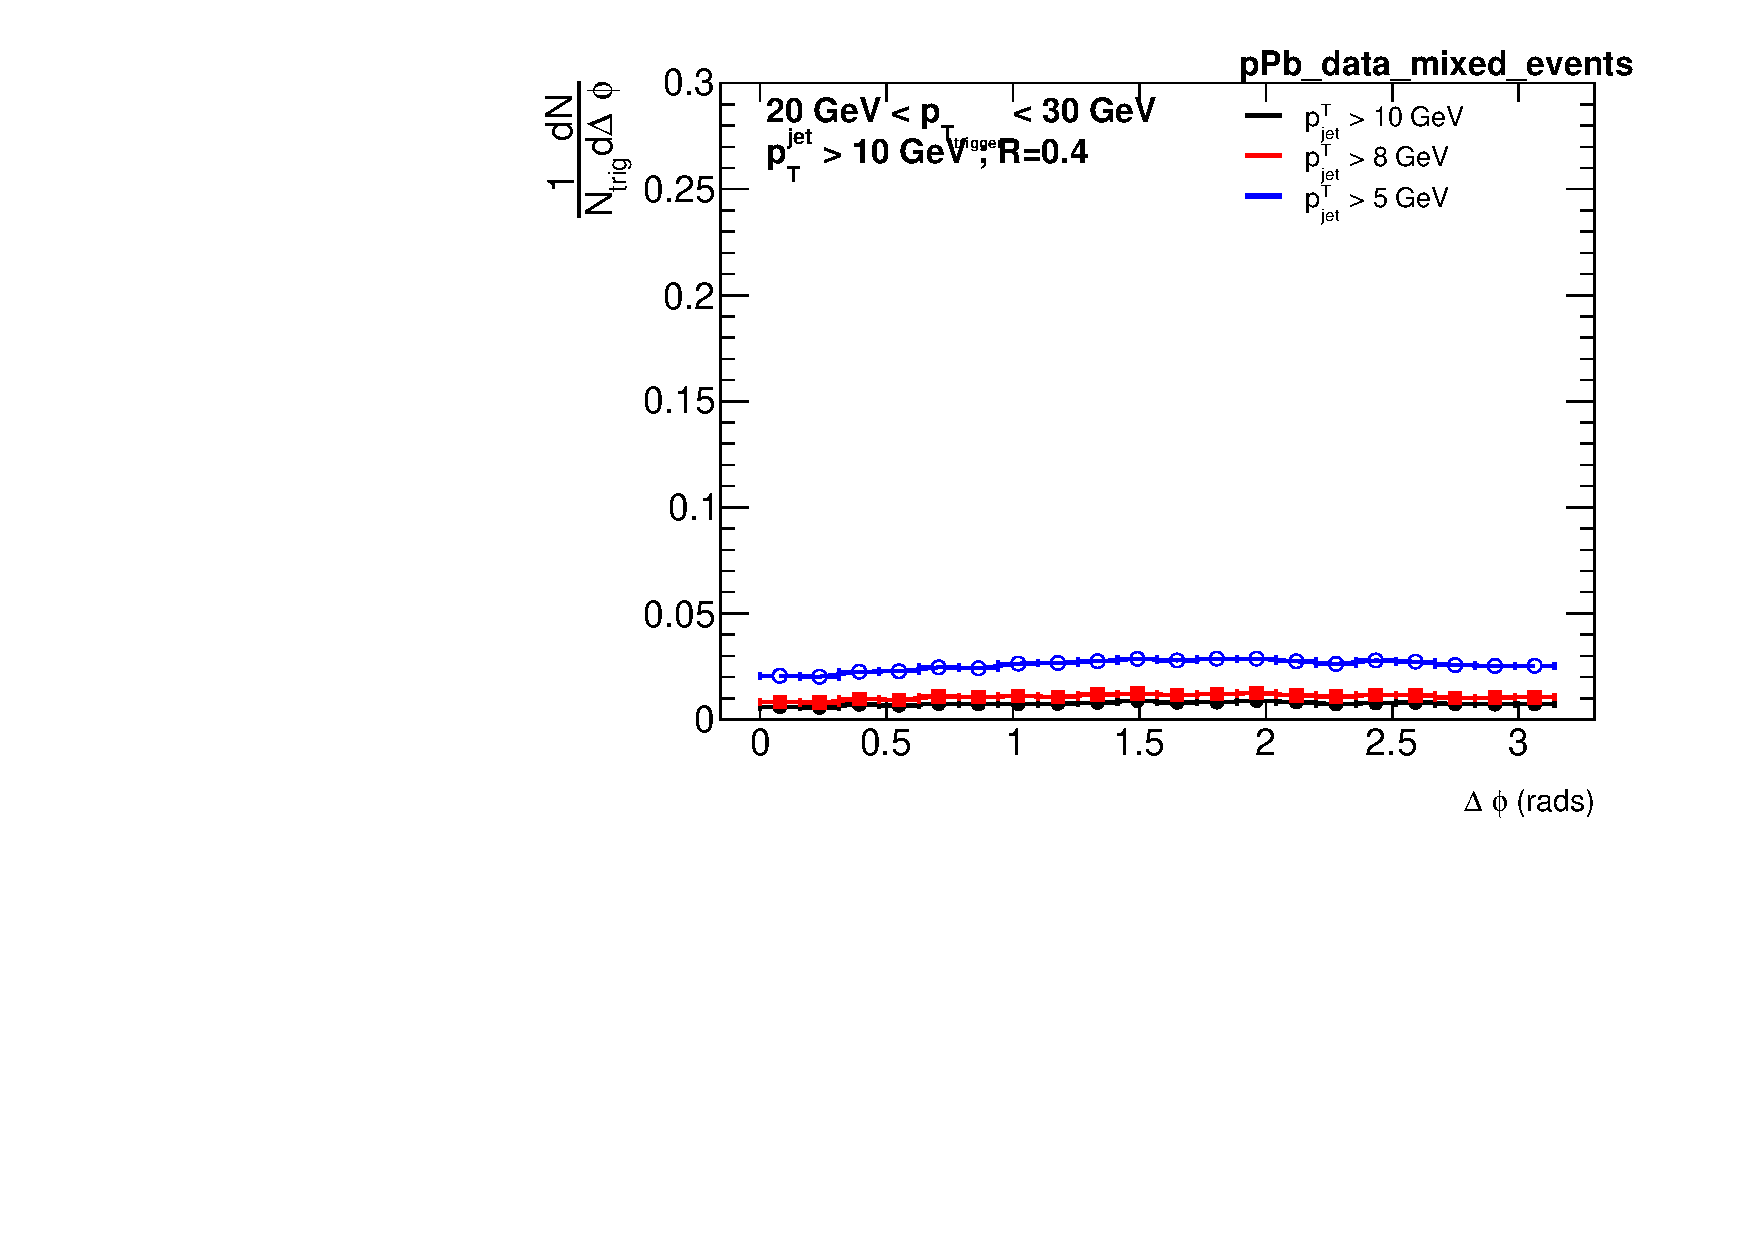
\includegraphics[width=0.495\textwidth]{GammaJet/sig_dPhipPb_data_mixed_events_Comparison.pdf}
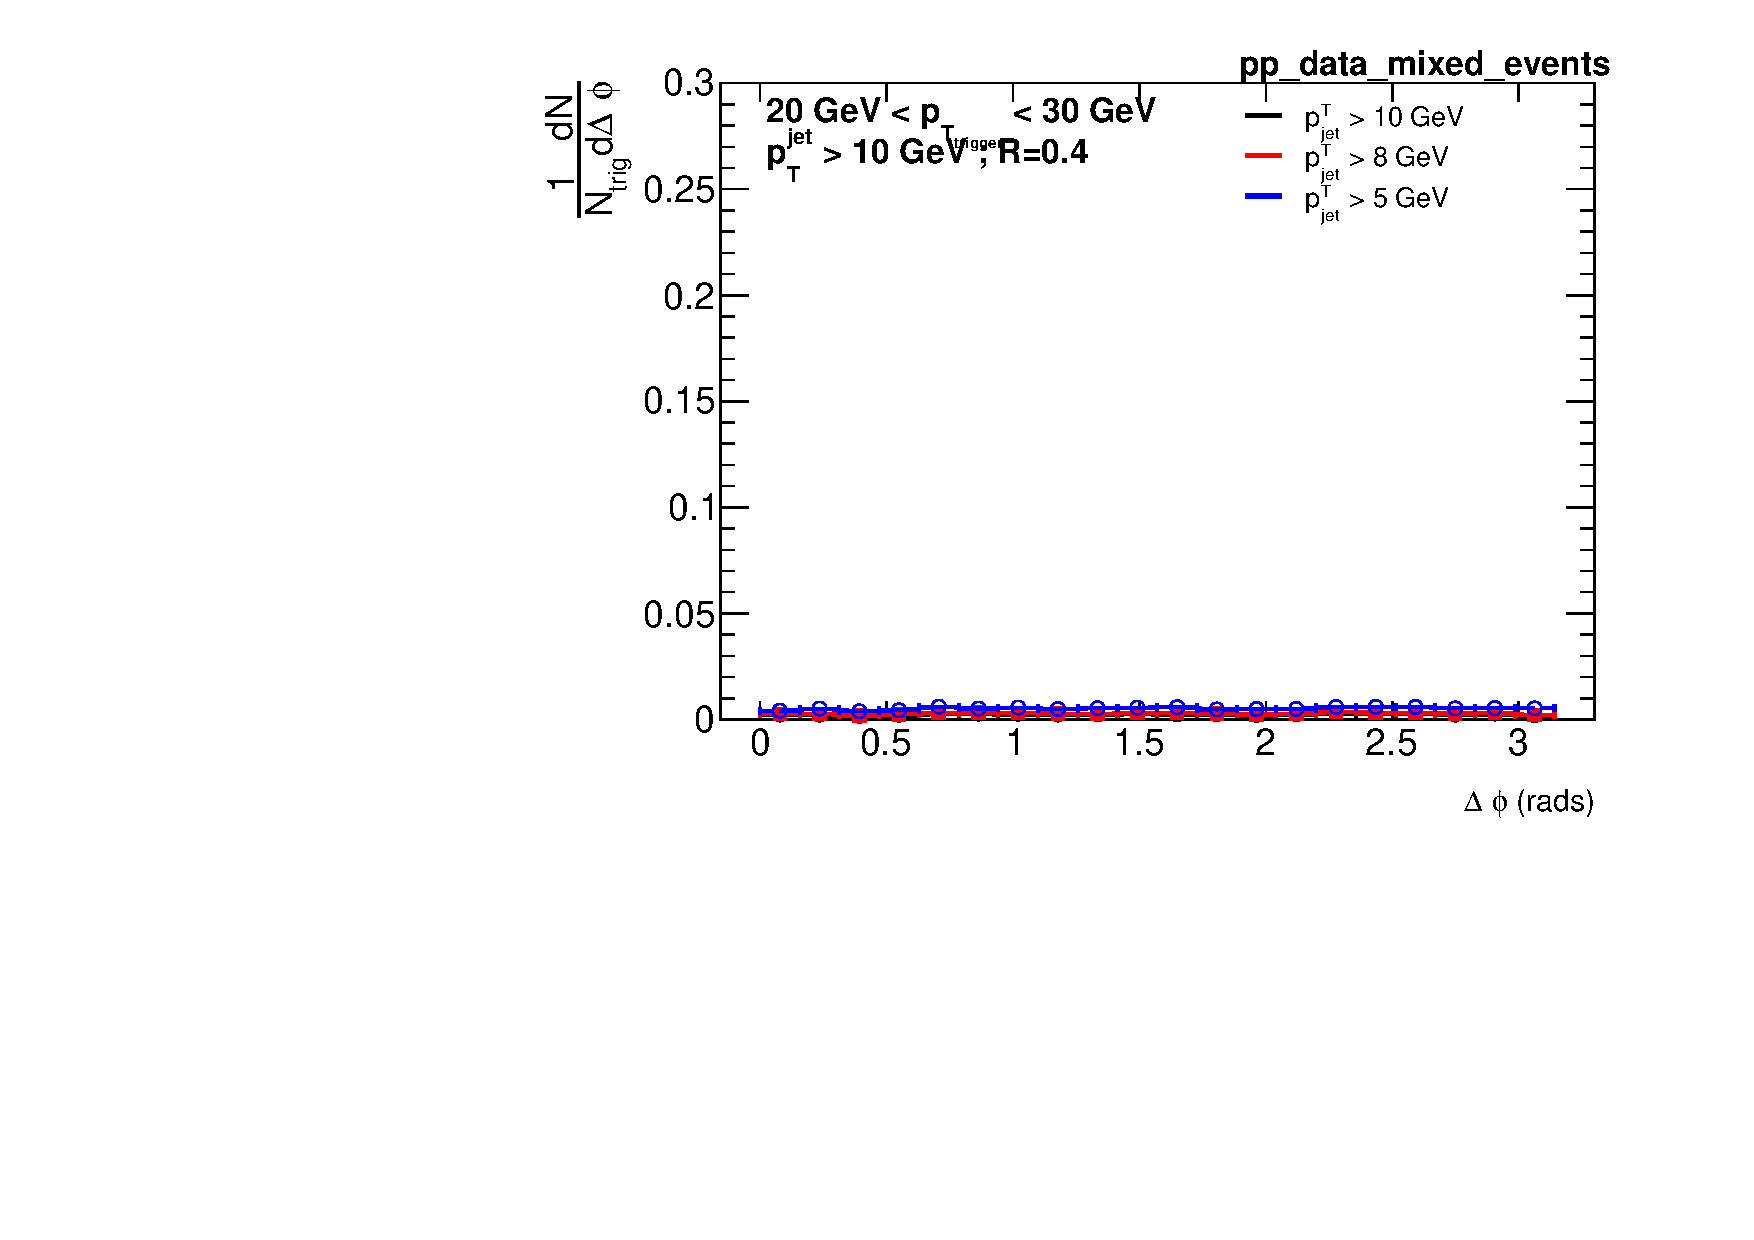
\includegraphics[width=0.495\textwidth]{GammaJet/sig_dPhipp_data_mixed_events_Comparison.pdf}
\caption{Coincidence rate, normalized per-photon and averaged over minimum-bias events, for cluster and jet pairs for various cuts on jet and cluster $\pt$ in p-Pb (left panel) and pp data (right panel). As explained in the main text, this is obtained with the event mixing technique.}
\label{4layerdPhi}
\end{figure}

\begin{figure}[h]
\centering
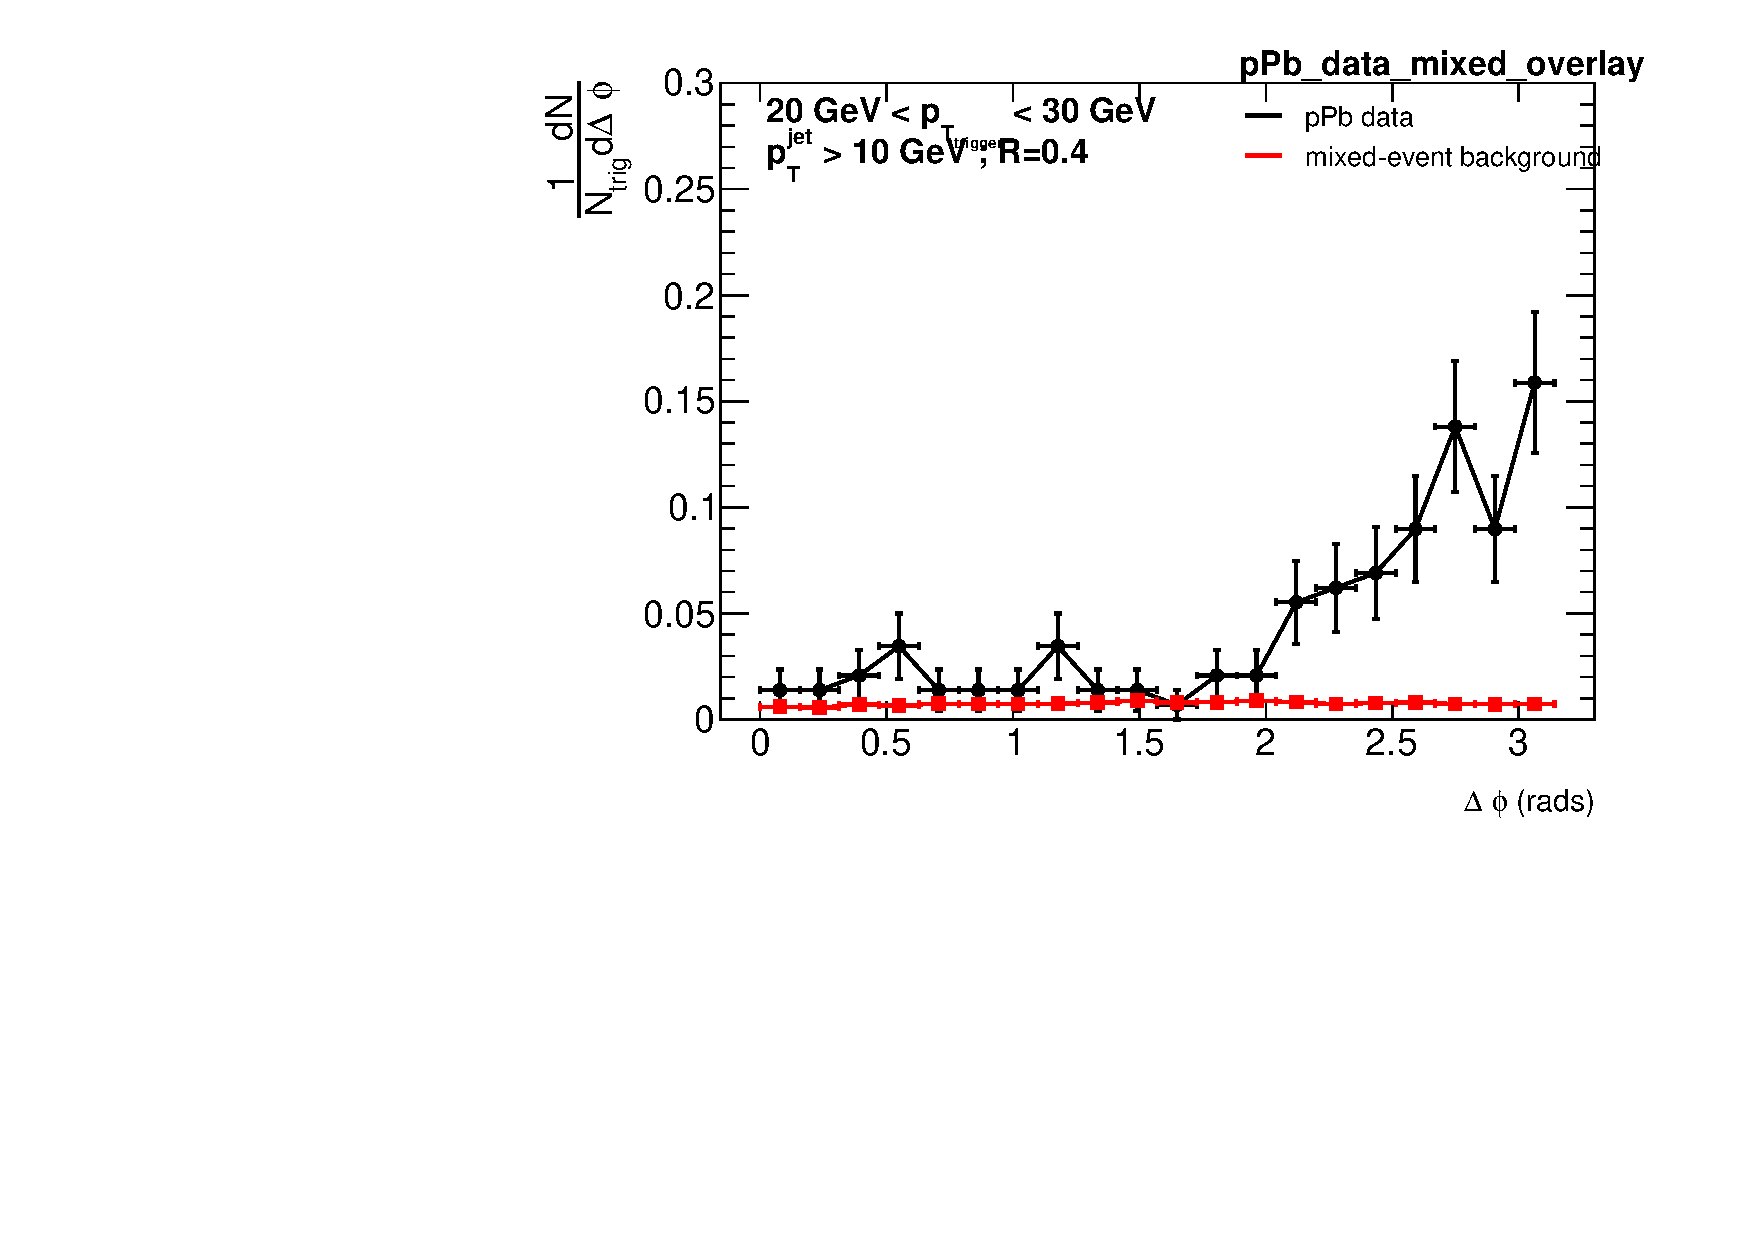
\includegraphics[width=0.495\textwidth]{GammaJet/sig_dPhipPb_data_mixed_overlay_Comparison.pdf}
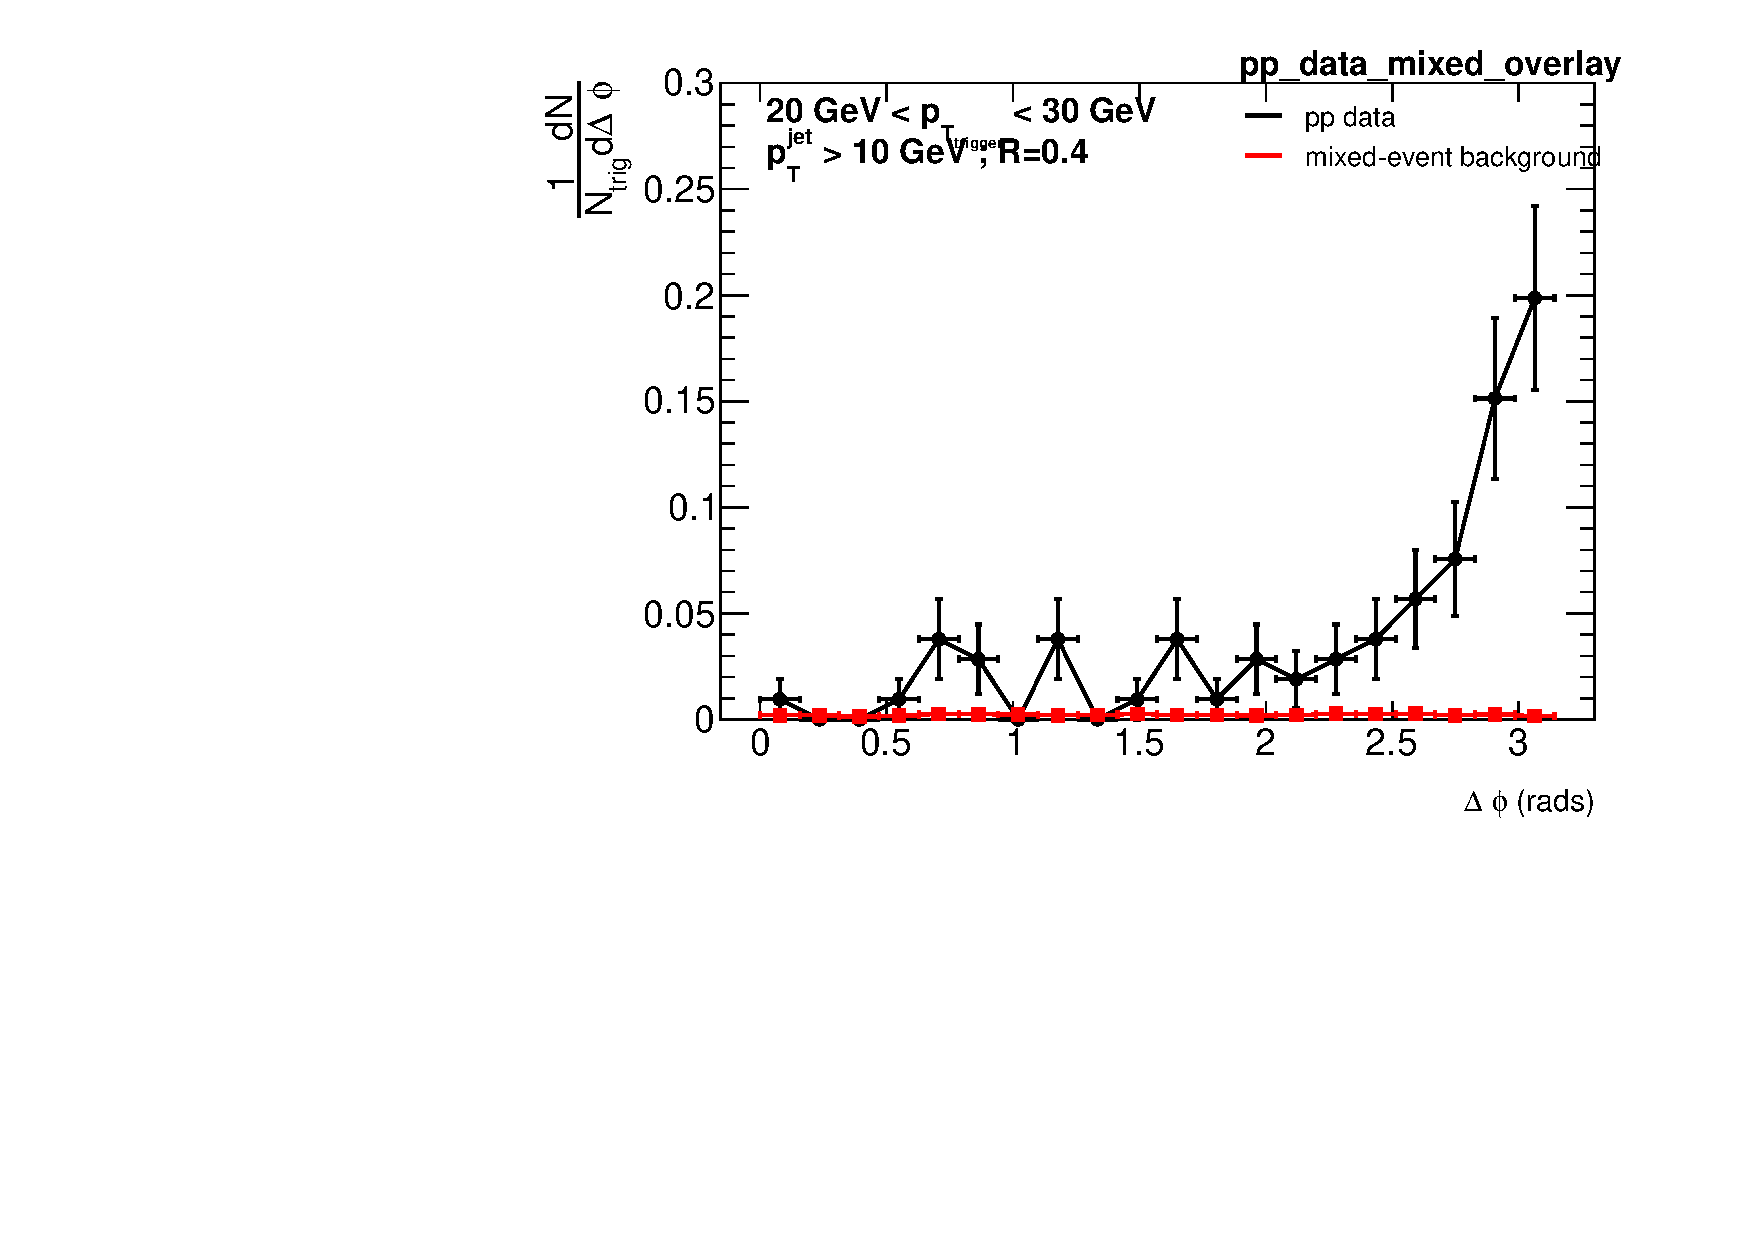
\includegraphics[width=0.495\textwidth]{GammaJet/sig_dPhipp_data_mixed_overlay_Comparison.pdf}
\caption{Comparison of $\gamma$-jet correlations over $\Delta \phi$ for data vs. Mixed event background for pp (17q) and p-Pb (13def) data for $\pt^{\mathrm{jet}}$ $>$ 10 GeV}
\label{fig:data_mixed_event_comparison}
\end{figure}

\begin{table}[h]
\caption{Background fraction in data in p-Pb and pp data for $p_{T}^{jet}$ $>$ 10 \GeVc~for $\frac{2 \pi}{3}$ $<$ $\Delta \phi$ $<$ $\pi$. This is estimated by the event-mixing technique as shown in the correlations of Figure~\ref{fig:data_mixed_event_comparison}}
\centering
\begin{tabular}{c c c c}
\hline
Data samples & Jet radius & Mixed/Data Ratio for $\frac{\pi}{2}$ $<$ $\Delta \phi$ $<$ $\pi$ & Mixed/Data Ratio for $\frac{2 \pi}{3}$ $<$ $\Delta \phi$ $<$ $\pi$ \\
\hline
pp & R=0.4&  0.6\% & 0.5\% \\
p-Pb & R=0.4& 16.5\% & 12.3\% \\
[1ex]
\hline
\end{tabular}
\label{tab:MixedEventBackgroundRatios}
\end{table}

In Figure~\ref{4layerdPhi}, the $\Delta \phi$ distributions of the pairs are shown to be relatively constant, though tighter cuts on jet $\pt$ reduces the magnitude of the the distribution (the $>$5 \GeVc~to $>$7.5~\GeVc~shift in particular). All rates measured in pp collisions are smaller than the corresponding ones for p-Pb collisions, as expected. 

As shown in Figure \ref{fig:data_mixed_event_comparison} and Table \ref{tab:MixedEventBackgroundRatios}, the ratio between the mixed-event background and data is very small, on the order of 0.5\%, which suggests that the background due to random combinations of high $\pt$ photons and jets with $\pt>$ 10 \GeVc~is negligible for pp collisions. However, the corresponding background for p-Pb is not negligible. The p-Pb mixed-event background is between 12\% and 17\% of the p-Pb data, depending on the $\Delta\varphi$ range chosen. As expected, constricting the sampled azimuthal angle difference interval from $\frac{\pi}{2}$ $<$ $\Delta \phi$ $<$ $\pi$ to $\frac{2 \pi}{3}$ $<$ $\Delta \phi$ $<$ $\pi$ reduced the ratios, but not significantly (0.00626 to 0.005 for pp, 0.165 to 0.123 for p-Pb).


\subsection{Results}
\label{sec:GammaJetResults}
In this section, we discuss the results of the primary correlation procedure outlined in Section \ref{sec:GammaJetProcedure}.
\subsubsection{$x^{obs}_{Pb}$}
\label{sec:GammaJetResultsxobsPb}
In this section, we present the correlations with respect to the Bjorken-x-sensitive observable $x^{obs}_{Pb}$. It is defined in Equation \ref{eq:xobsPb}:
\begin{equation}
    x^{obs}_{Pb} \equiv \frac{p_{T}^{\gamma}e^{-\eta^{\gamma}}+p_{T}^{jet}e^{-\eta^{jet}}}{2E_{Pb}}
    \label{eq:xobsPb}
\end{equation}
Where $p_{T}^{\gamma}$ and $\eta^{\gamma}$ are the transverse momentum and pseudorapidity of the photon in the $\gamma$-jet pair, respectively, and  $p_{T}^{jet}$ and $\eta^{jet}$ are the corresponding quantities of the jet. $E_{Pb}$ is the energy of the lead nucleus in our pPb collision, which take to be 1560 MeV. This observable is particularly important, because it helps to probe the distribution of hard scattering events at low Bjorken-x.  

Figure \ref{fig:xobsPbdata} shows a comparison of the $\gamma$-jet correlation with respect to $x^{obs}_{Pb}$ for pp and pPb.

\begin{figure}
    \centering
    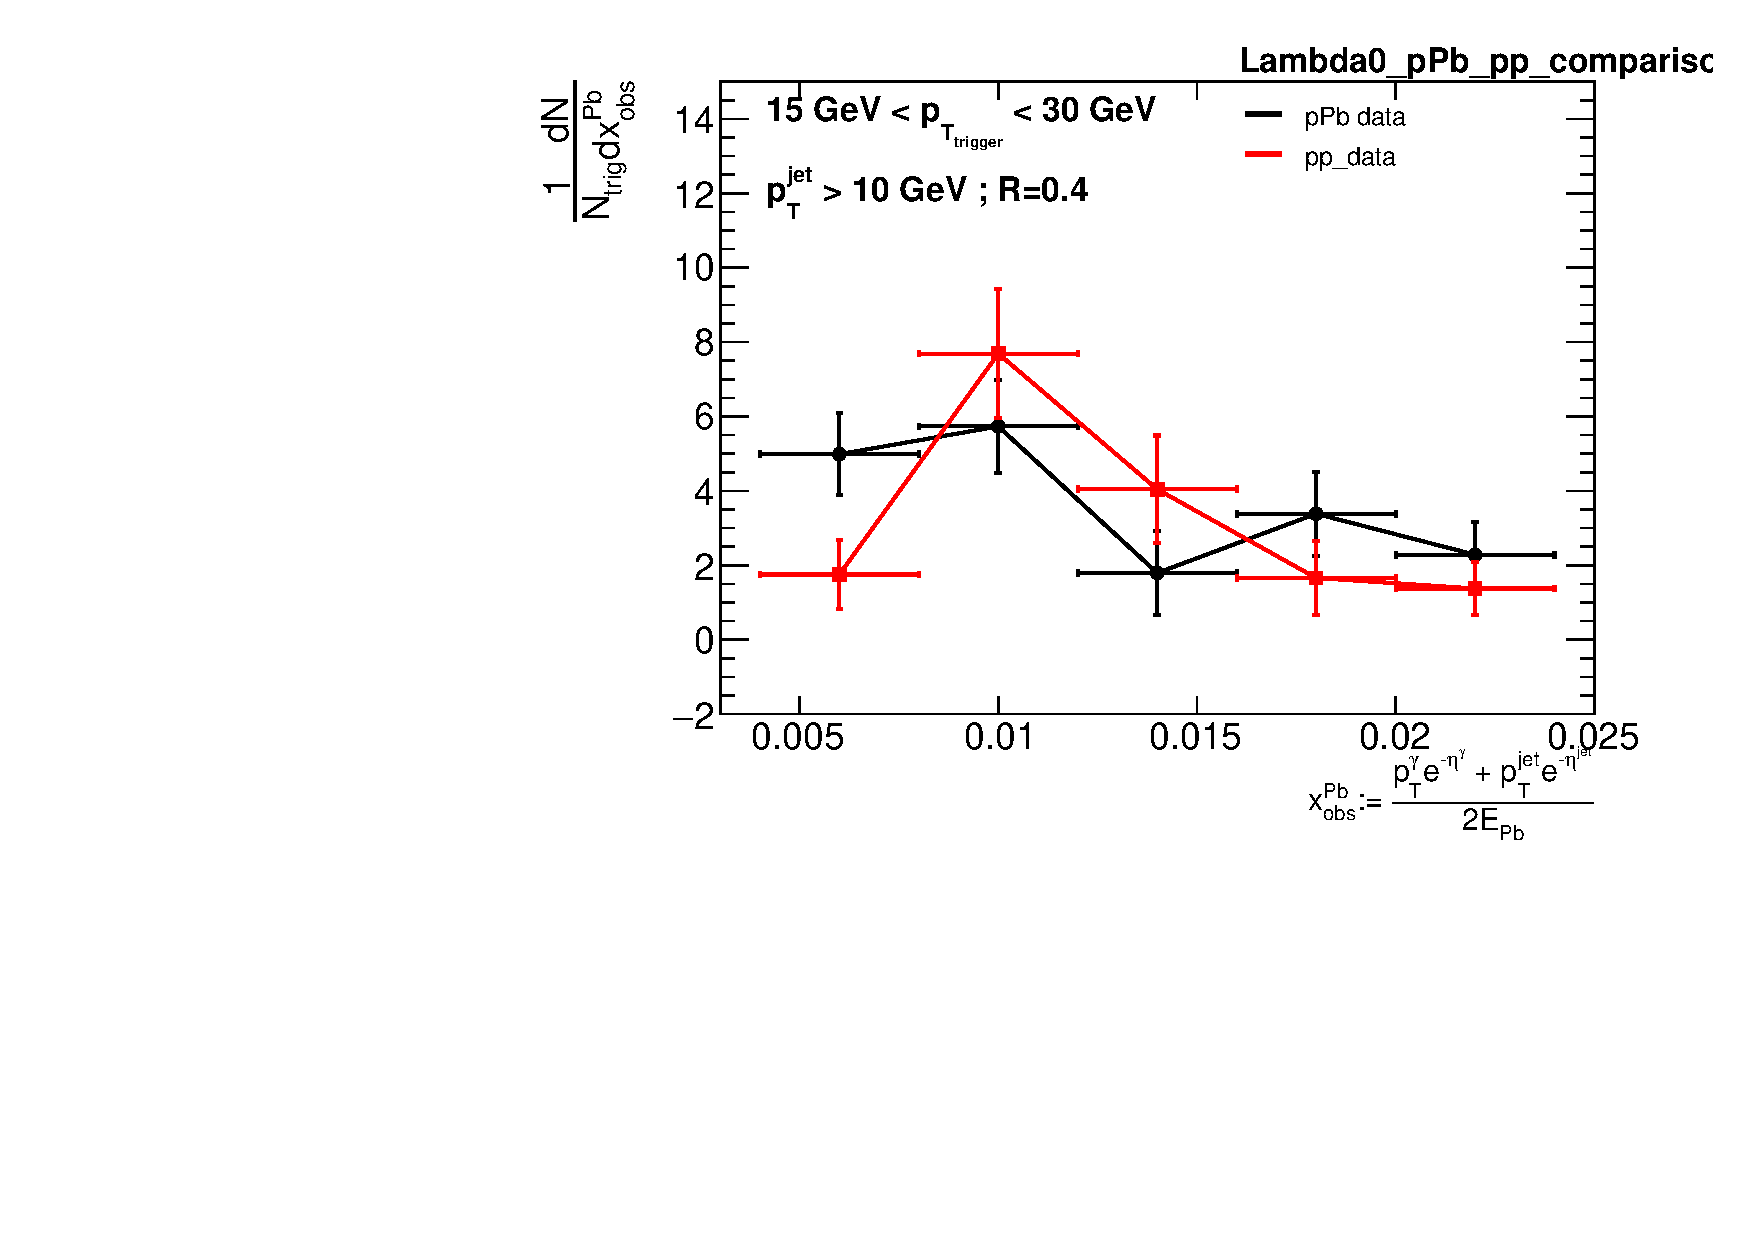
\includegraphics[width=0.49\textwidth]{GammaJet/pp_pPb_correlations/hadj_XobsPbLambda0_pPb_pp_comparison_Comparison.pdf}
    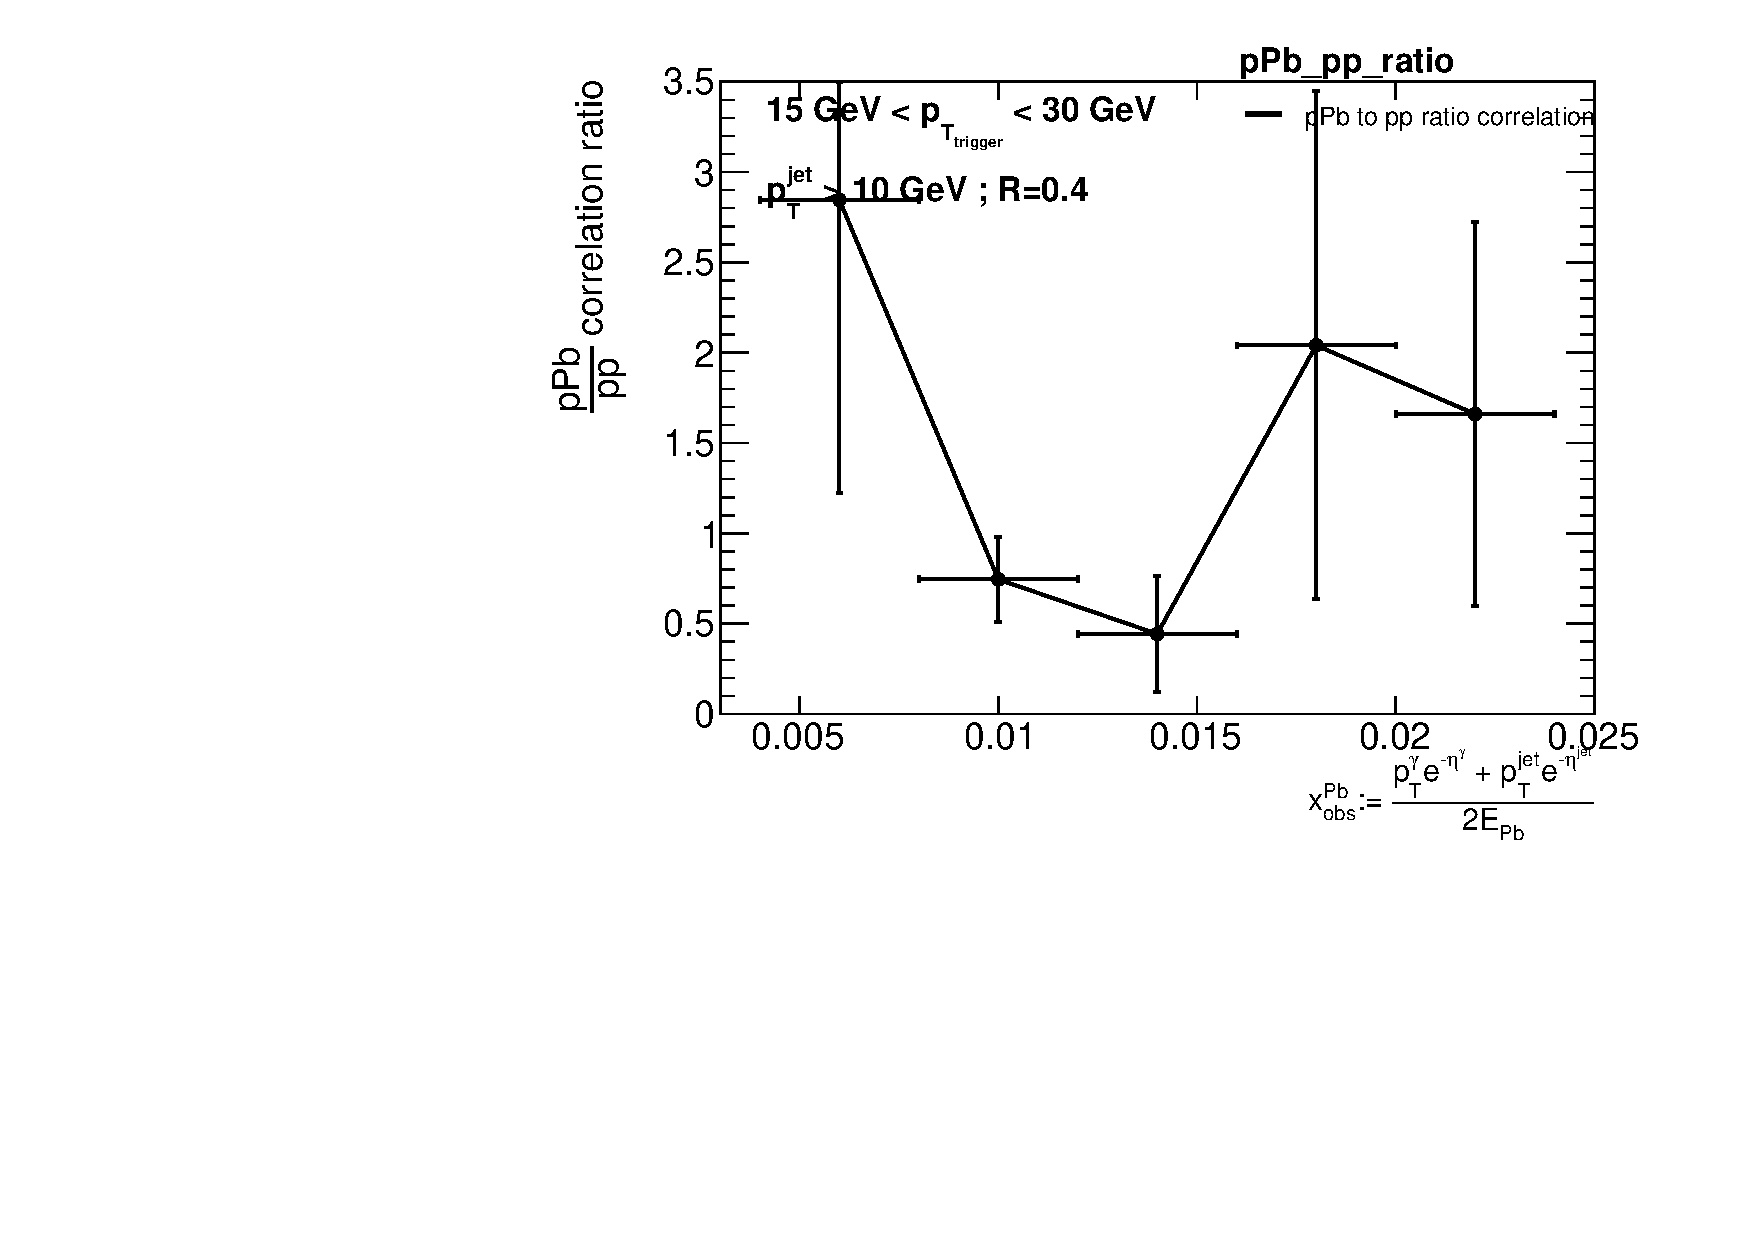
\includegraphics[width=0.49\textwidth]{GammaJet/pp_pPb_correlations/hadj_XobsPb_ratiopPb_pp_ratio_Comparison.pdf}
    \caption{A comparison of the $x^{obs}_{Pb}$ correlations for pp and pPb. The correlations themselves are on the left, the $\frac{pPb}{pp}$ correlation ratio is on the right.}
    \label{fig:xobsPbdata}
\end{figure}

As seen in Figure \ref{fig:xobsPbdata}, both the pp and the pPb data show a peak at $x^{obs}_{Pb}$=0.01, though pp shows a secondary peak at $x^{obs}_{Pb}$=0.02. Nonetheless, the pp and pPb correlations are generally within uncertainty of one another. This could be due to the large error bars: the subtraction in Equation \ref{eq:FinalSubtraction} reduces the number of $\gamma$-jet pairs considered to a very small number, usually less than 100 for a typical sample. This naturally results in large error bars. This becomes more apparent in the correlation ratio (especially at off-peak $x^{obs}_{Pb}$ values.

Hopefully future runs with an upgraded ALICE, which will contain more data, will help remedy this. Nonetheless, the current results help to constrain the distribution of hard-scattering events at low Bjorken-x. 

\subsubsection{Other observables}
In this section, we present the $\gamma$-jet correlations in pp and pPb in other observables. The most important of these observables is $\Delta \phi$, the results of which are shown in Figure \ref{fig:dPhidata}.

The other observables are $X_j$ (which is $\frac{p_T^{jet}}{p_T^{\gamma}}$), jet multiplicity, and $p_TD$, which is a measure of jet $p_T$ dispersion. The results of these observables are shown in Figure \ref{fig:other_obs_data}.

\begin{figure}
    \centering
    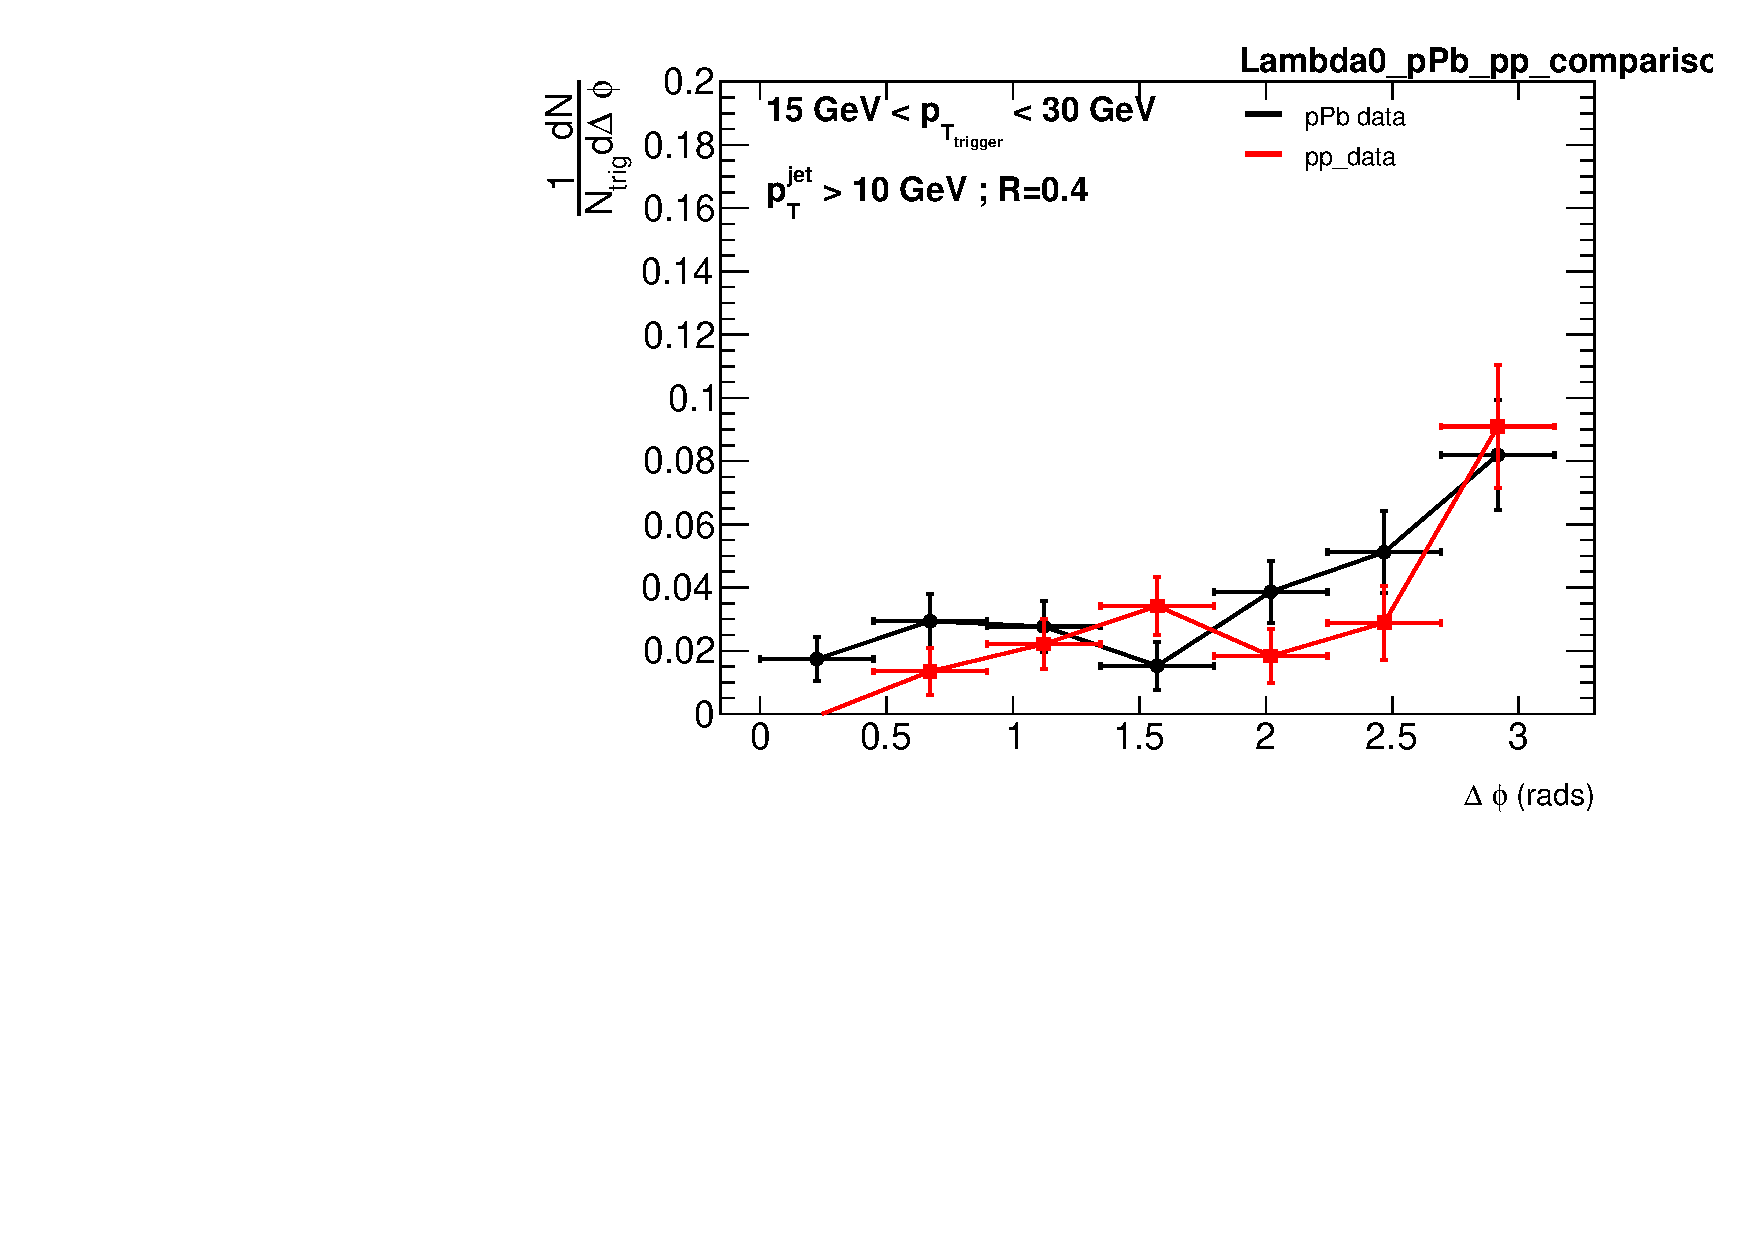
\includegraphics[width=0.49\textwidth]{GammaJet/pp_pPb_correlations/hadj_dPhiLambda0_pPb_pp_comparison_Comparison.pdf}
    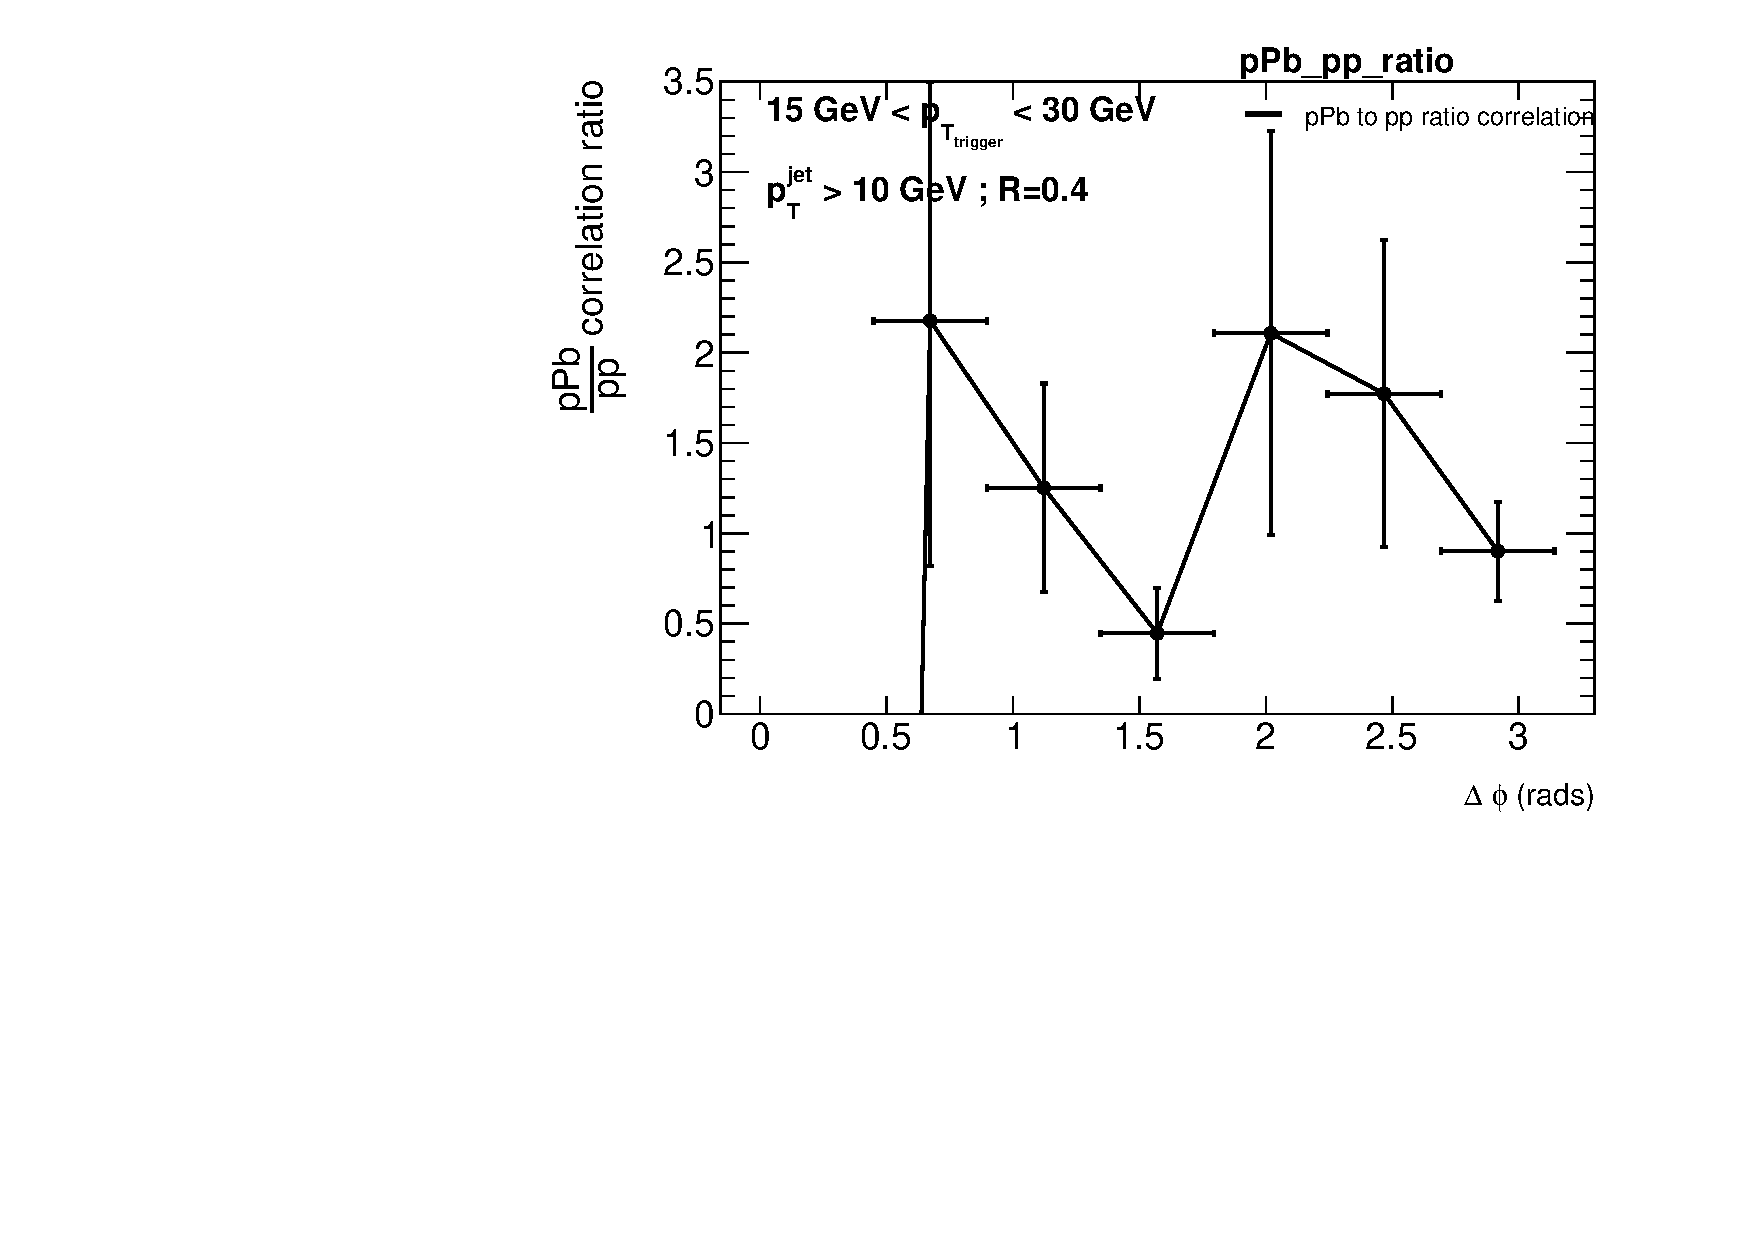
\includegraphics[width=0.49\textwidth]{GammaJet/pp_pPb_correlations/hadj_dPhi_ratiopPb_pp_ratio_Comparison.pdf}
    \caption{A comparison of the $\Delta \phi$ correlations for pp and pPb. The correlations themselves are on the left, the $\frac{pPb}{pp}$ correlation ratio is on the right.}
    \label{fig:dPhidata}
\end{figure}

\begin{figure}
    \centering
    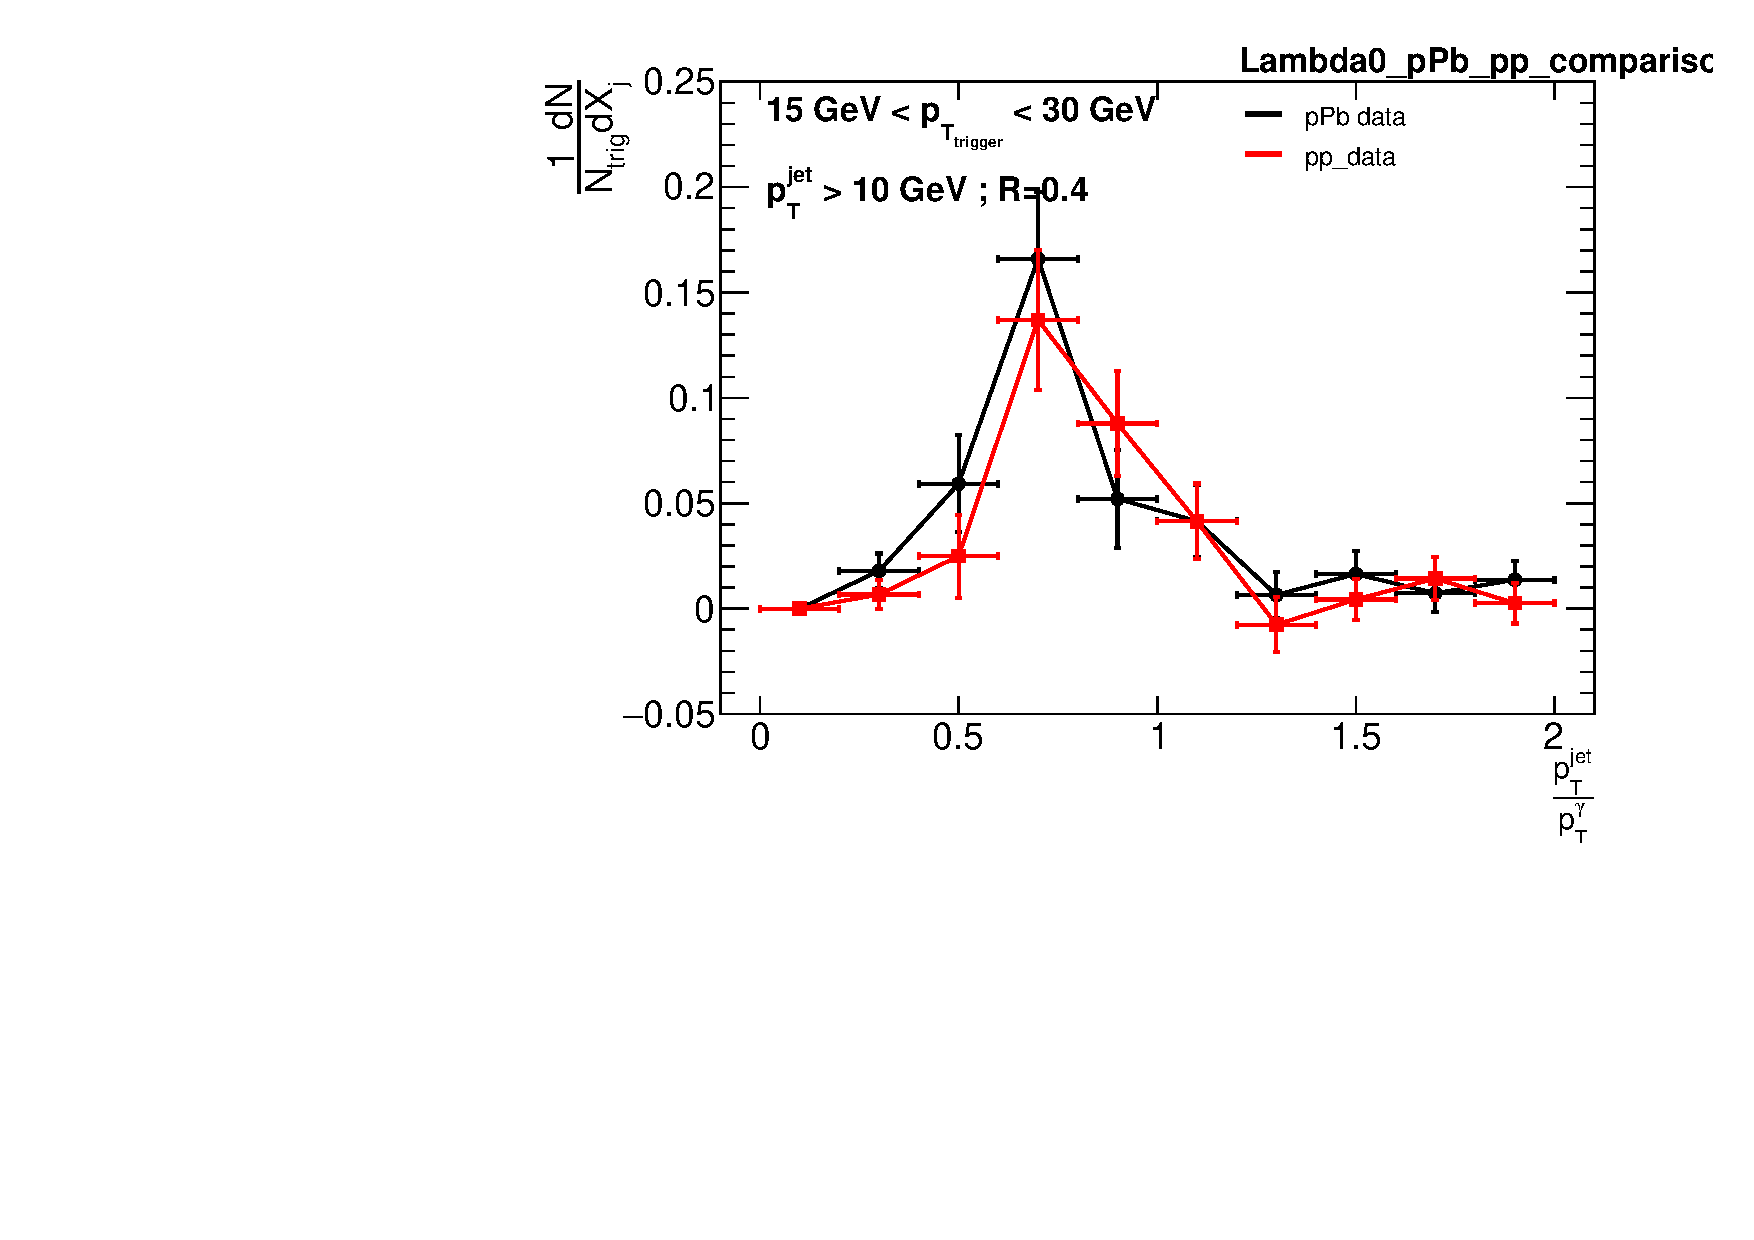
\includegraphics[width=0.32\textwidth]{GammaJet/pp_pPb_correlations/hadj_XjLambda0_pPb_pp_comparison_Comparison.pdf}
    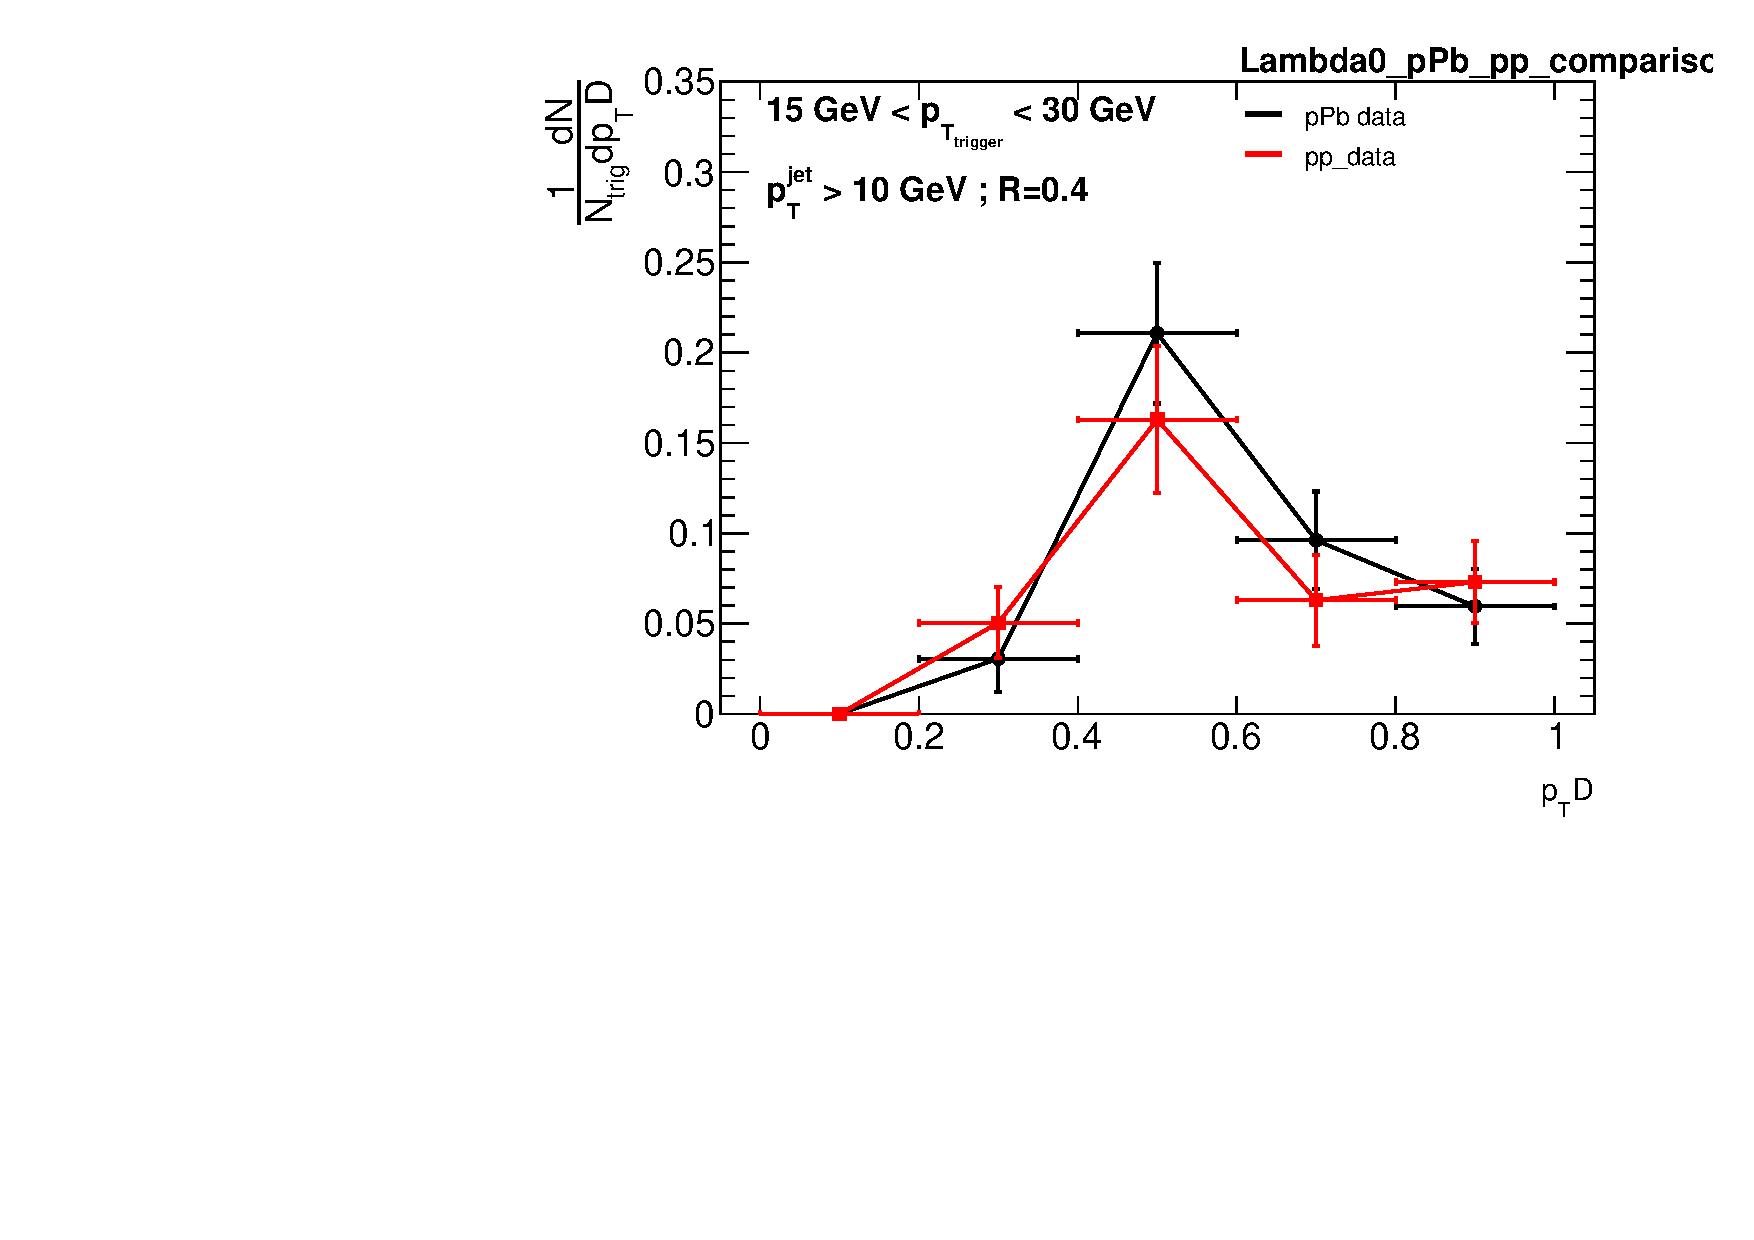
\includegraphics[width=0.32\textwidth]{GammaJet/pp_pPb_correlations/hadj_pTDLambda0_pPb_pp_comparison_Comparison.pdf}
    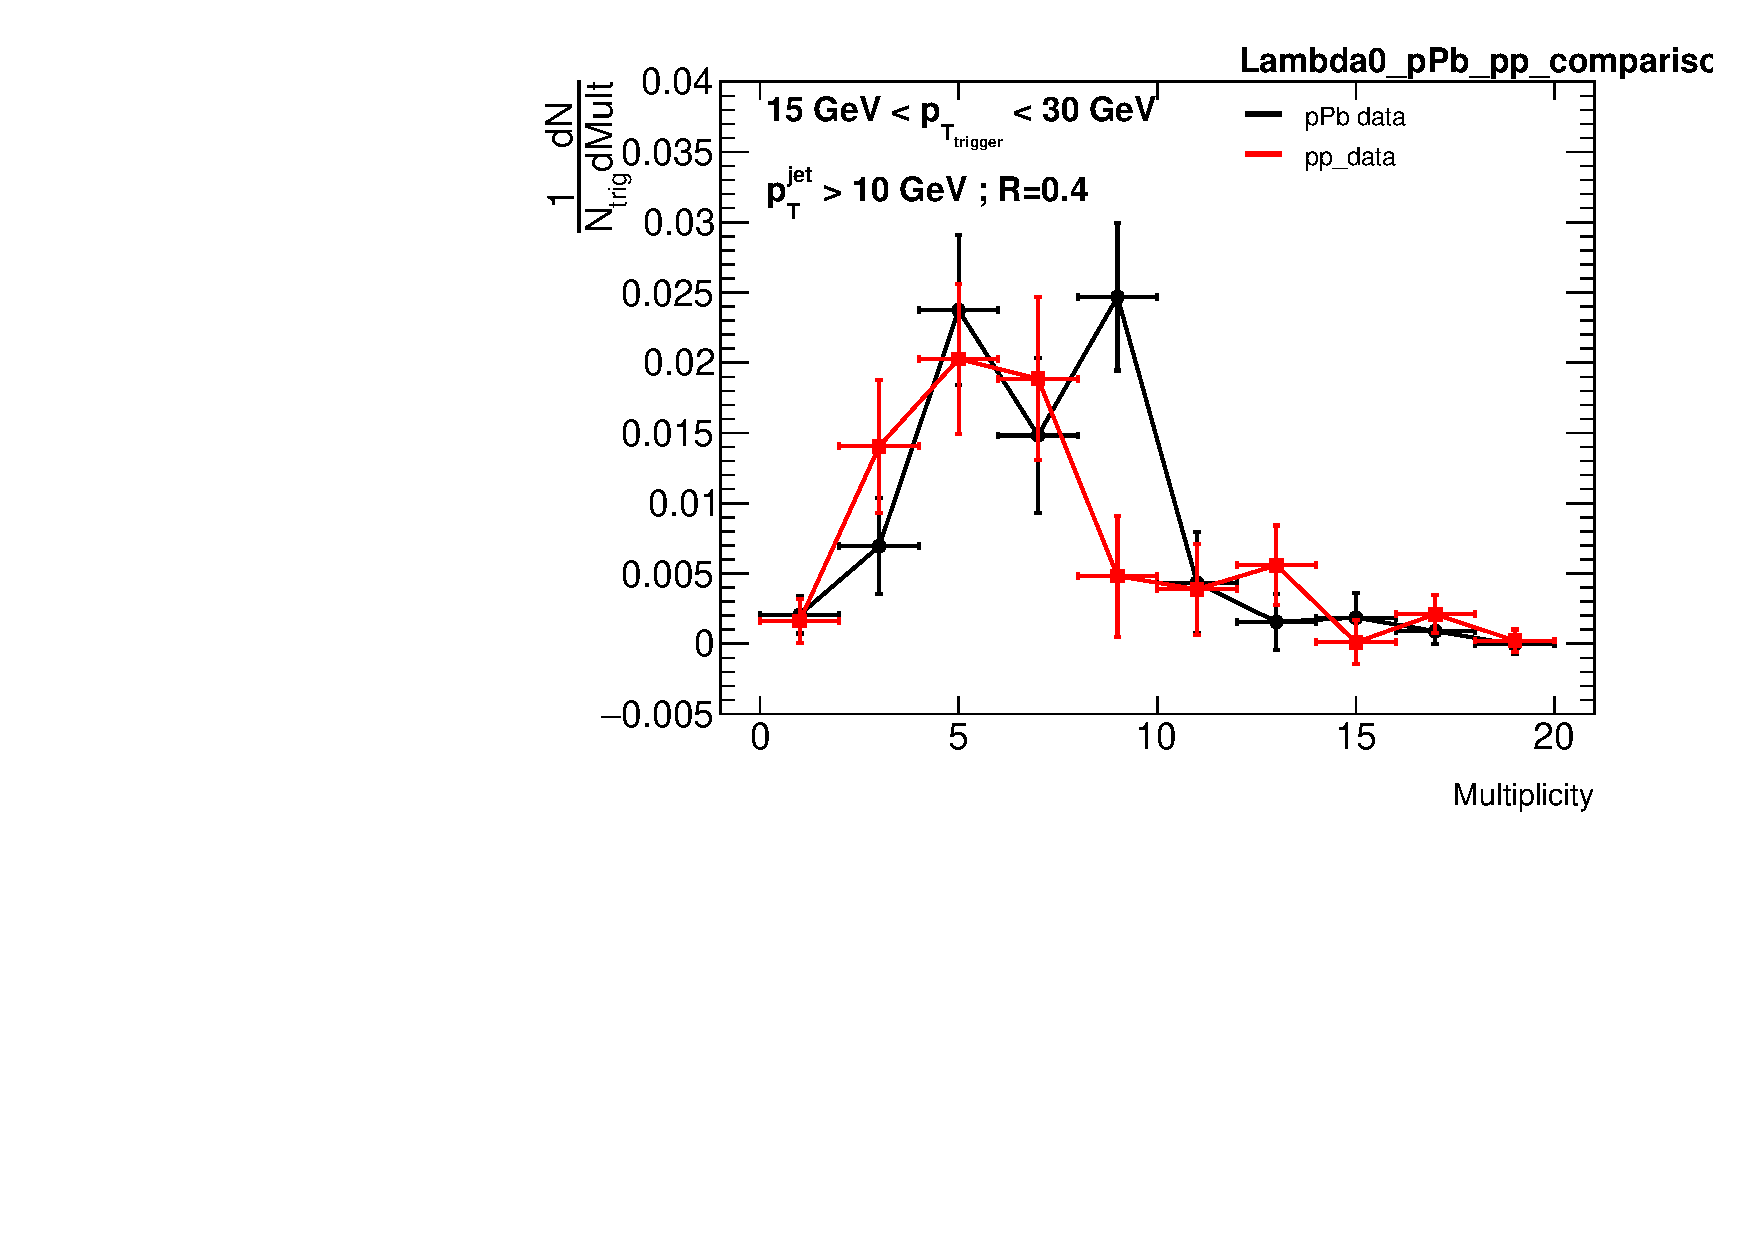
\includegraphics[width=0.32\textwidth]{GammaJet/pp_pPb_correlations/hadj_MultiplicityLambda0_pPb_pp_comparison_Comparison.pdf} \\
    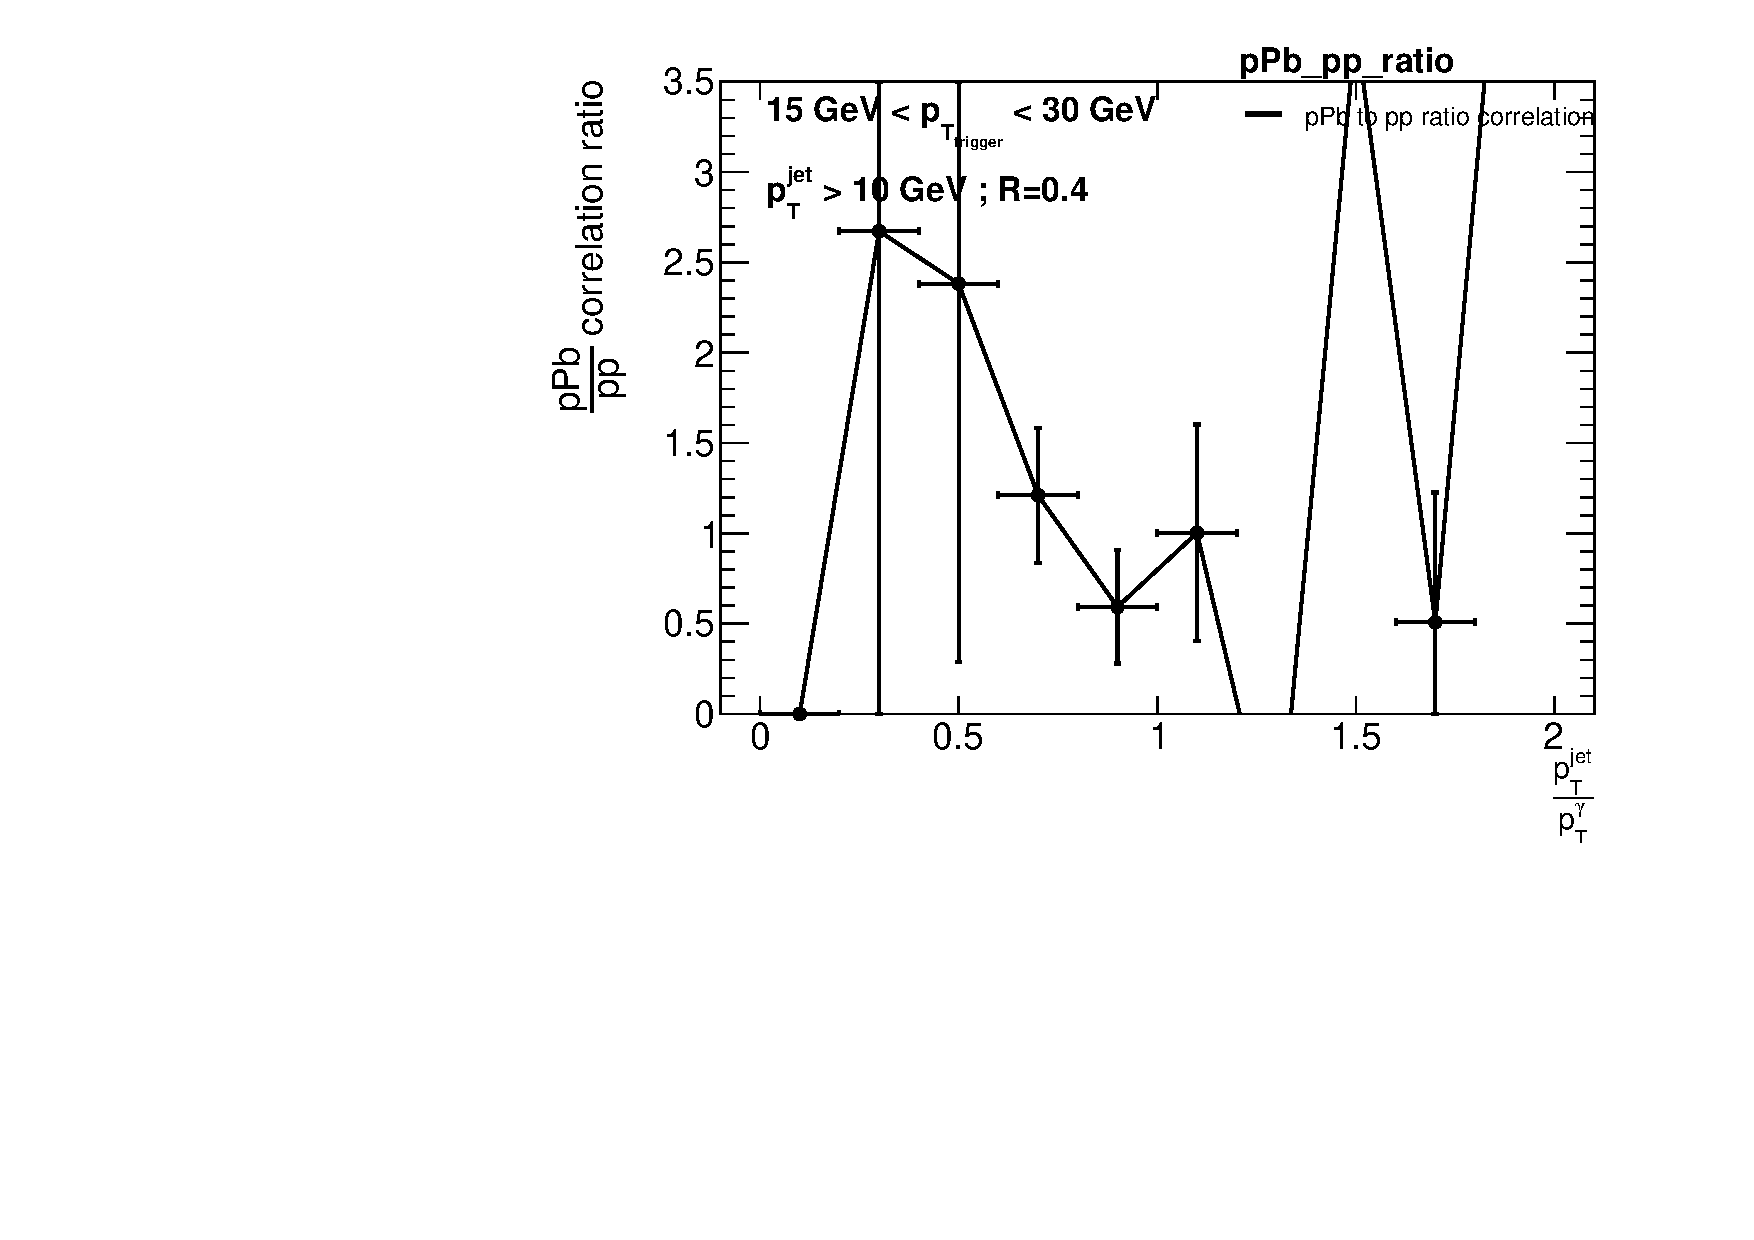
\includegraphics[width=0.32\textwidth]{GammaJet/pp_pPb_correlations/hadj_Xj_ratiopPb_pp_ratio_Comparison.pdf}
    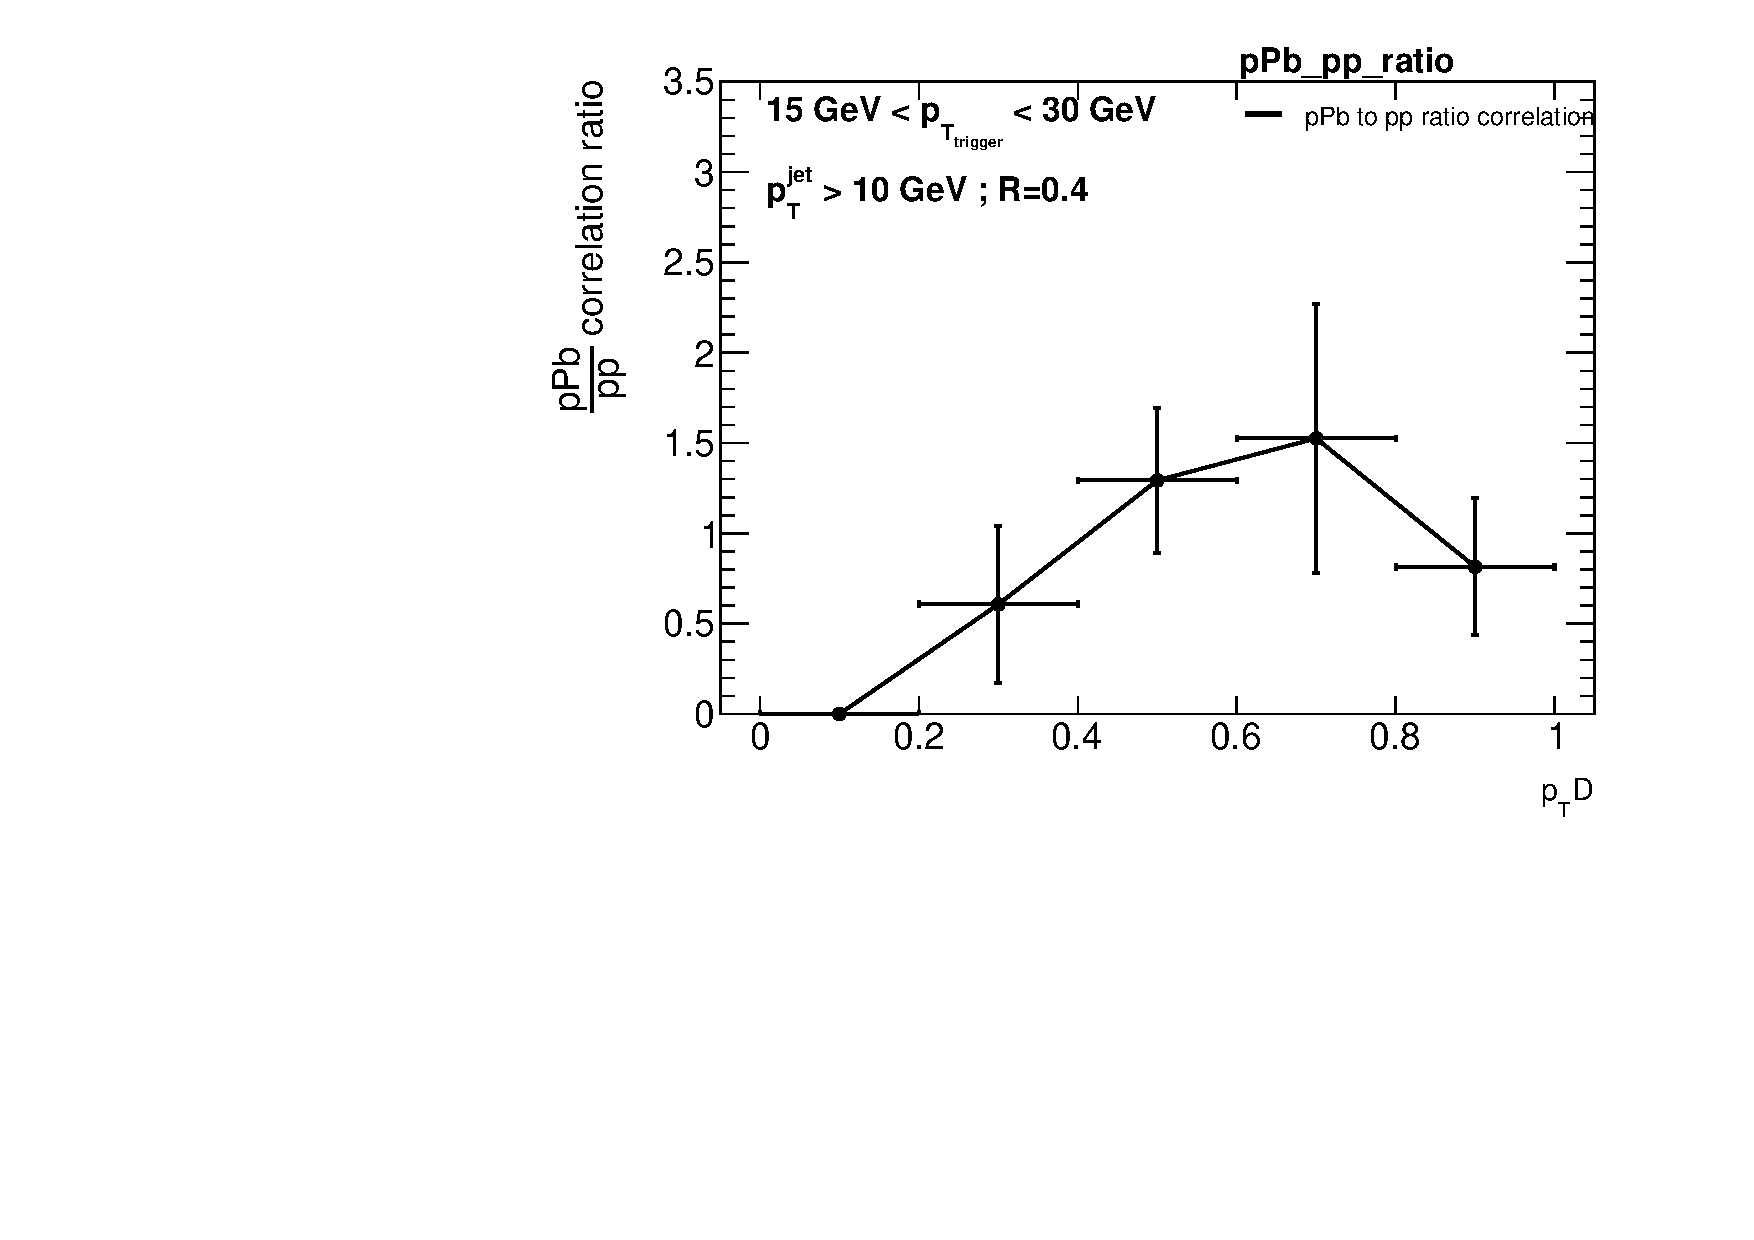
\includegraphics[width=0.32\textwidth]{GammaJet/pp_pPb_correlations/hadj_pTD_ratiopPb_pp_ratio_Comparison.pdf}
    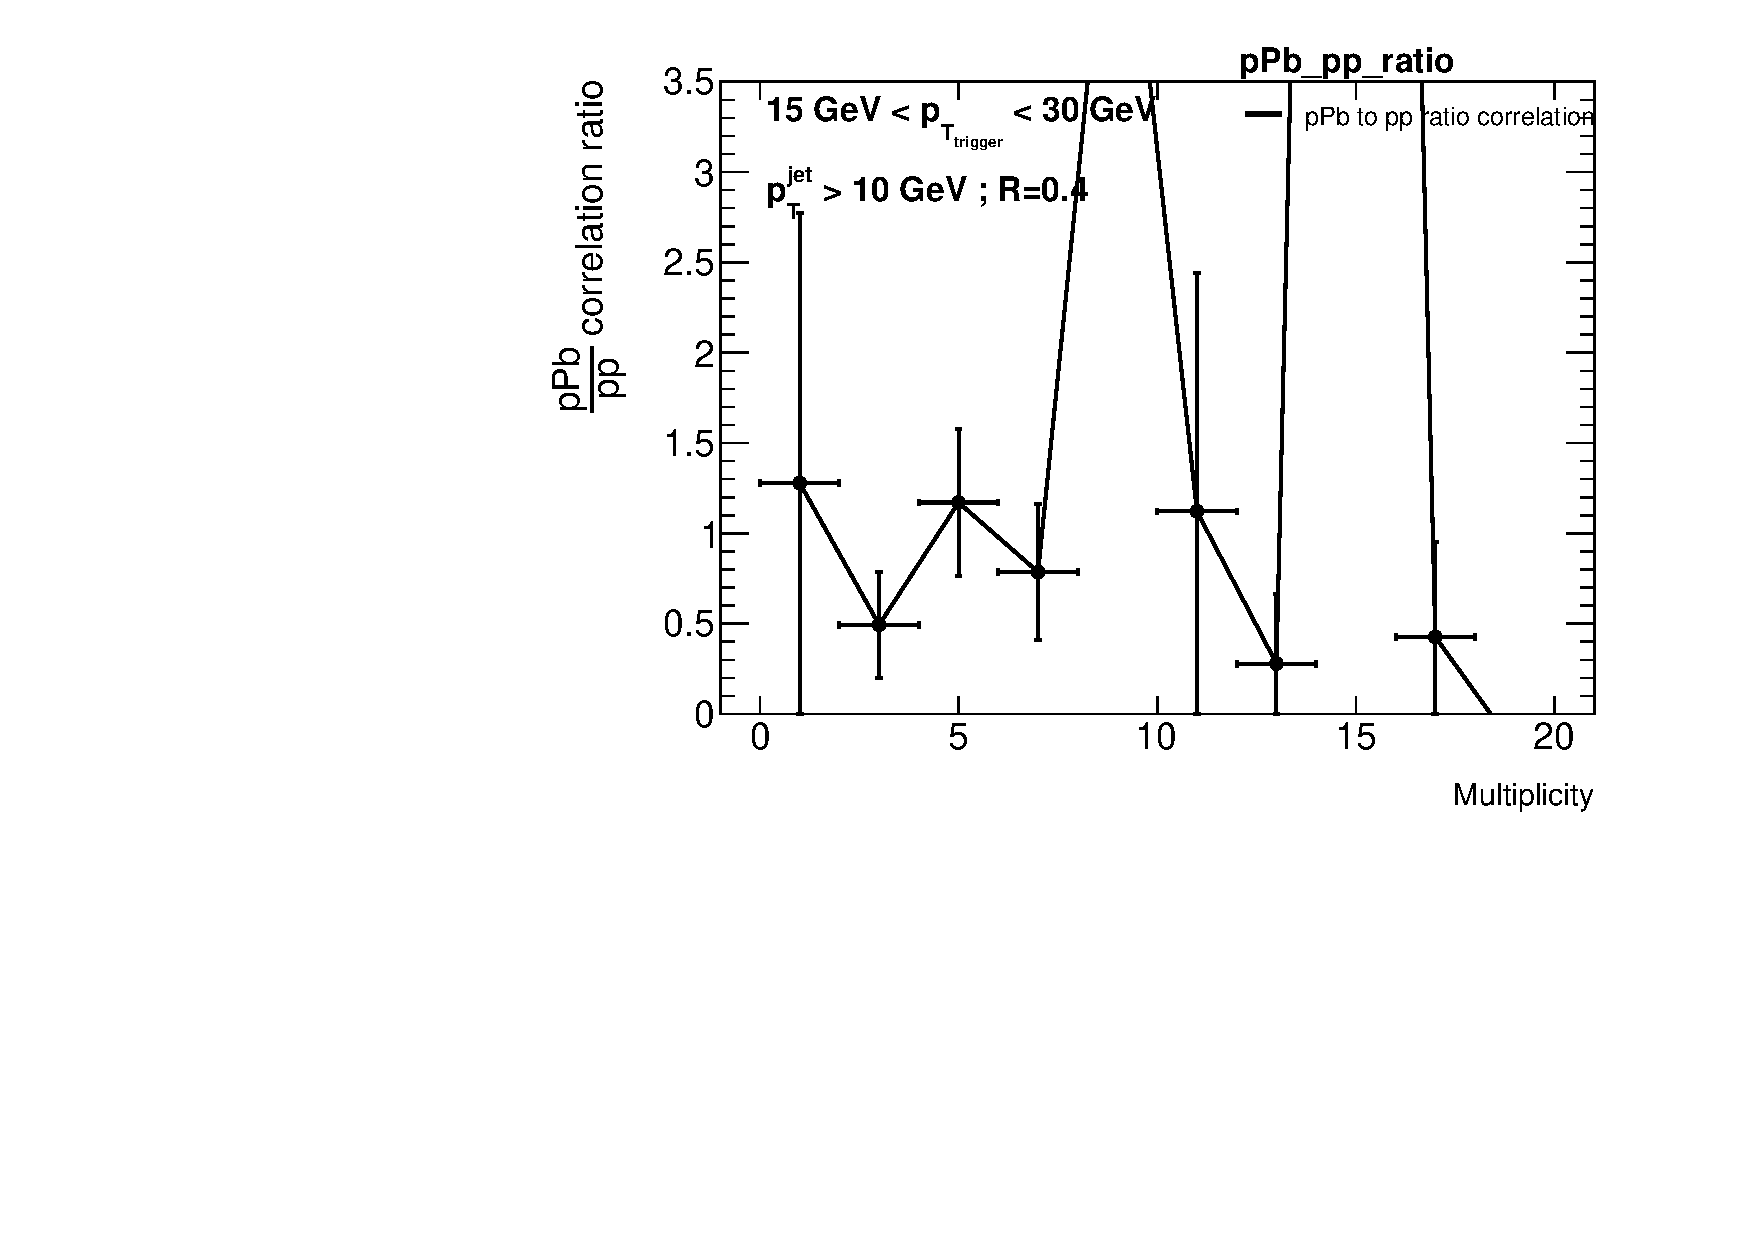
\includegraphics[width=0.32\textwidth]{GammaJet/pp_pPb_correlations/hadj_Multiplicity_ratiopPb_pp_ratio_Comparison.pdf}
    \caption{A comparison of pp and pPb $\gamma$-jet correlations for $X_j$ (left), $p_TD$ (center), and multiplicity (right). The correlations themselves are on the top, the $\frac{pPb}{pp}$ correlation ratio is on the bottom.}
    \label{fig:other_obs_data}
\end{figure}

As seen in Figures \ref{fig:dPhidata} and \ref{fig:other_obs_data}, the pp and the pPb correlations are within uncertainty of each other, just like for $x^{obs}_{Pb}$ in Section \ref{sec:GammaJetResultsxobsPb}. Also similar to $x^{obs}_{Pb}$ in Section \ref{sec:GammaJetResultsxobsPb}, the error bars are large, presumably for the same reasons. 

One important thing to note is that occasionally, the shower-shape background subtraction in Equation \ref{eq:FinalSubtraction} dips the value of the correlation function to slightly below 0, which leads to the $\frac{pPb}{pp}$ ratio taking unphysical values, below 0. This may be due to lack of data, or an underestimate of the purity.

Figure \ref{fig:isoGammaCandiJetCorr} shows a pp-pPb comparison of $\gamma$-jet correlations in $\Delta \phi$, this time in the cluster $p_{T}$ range of 20-30 \GeVc. For this correlation, the shower-shape background subtraction in Equation \ref{eq:FinalSubtraction} is not done, because the amount of data in the 20-30 \GeVc range is much less than that in the 15-30 \GeVc range. Since Equation \ref{eq:FinalSubtraction} takes away much of the data, this would often mean leaving insufficient data to do the analysis.

%Figure~\ref{fig:gammajetdphi} shows the azimuthal correlation between $\gammaiso$--candidates and jets in pp and p-Pb data. Figures \ref{fig:gammajetXobsPb}, \ref{fig:gammajetMultiplicity}, \ref{fig:gammajetpTD}, and \ref{fig:gammajetXj} show corresponding correlations, but with the following observables, in that order: $X_{obs}^{Pb}$, Multiplicity, $p_{T}D$, $X_j$. This includes both correlations before the subtraction of correlations with $\ydecay$ using Equation $\ref{eq:32}$ and after the said subtraction
%\begin{figure}[h]
%\center
%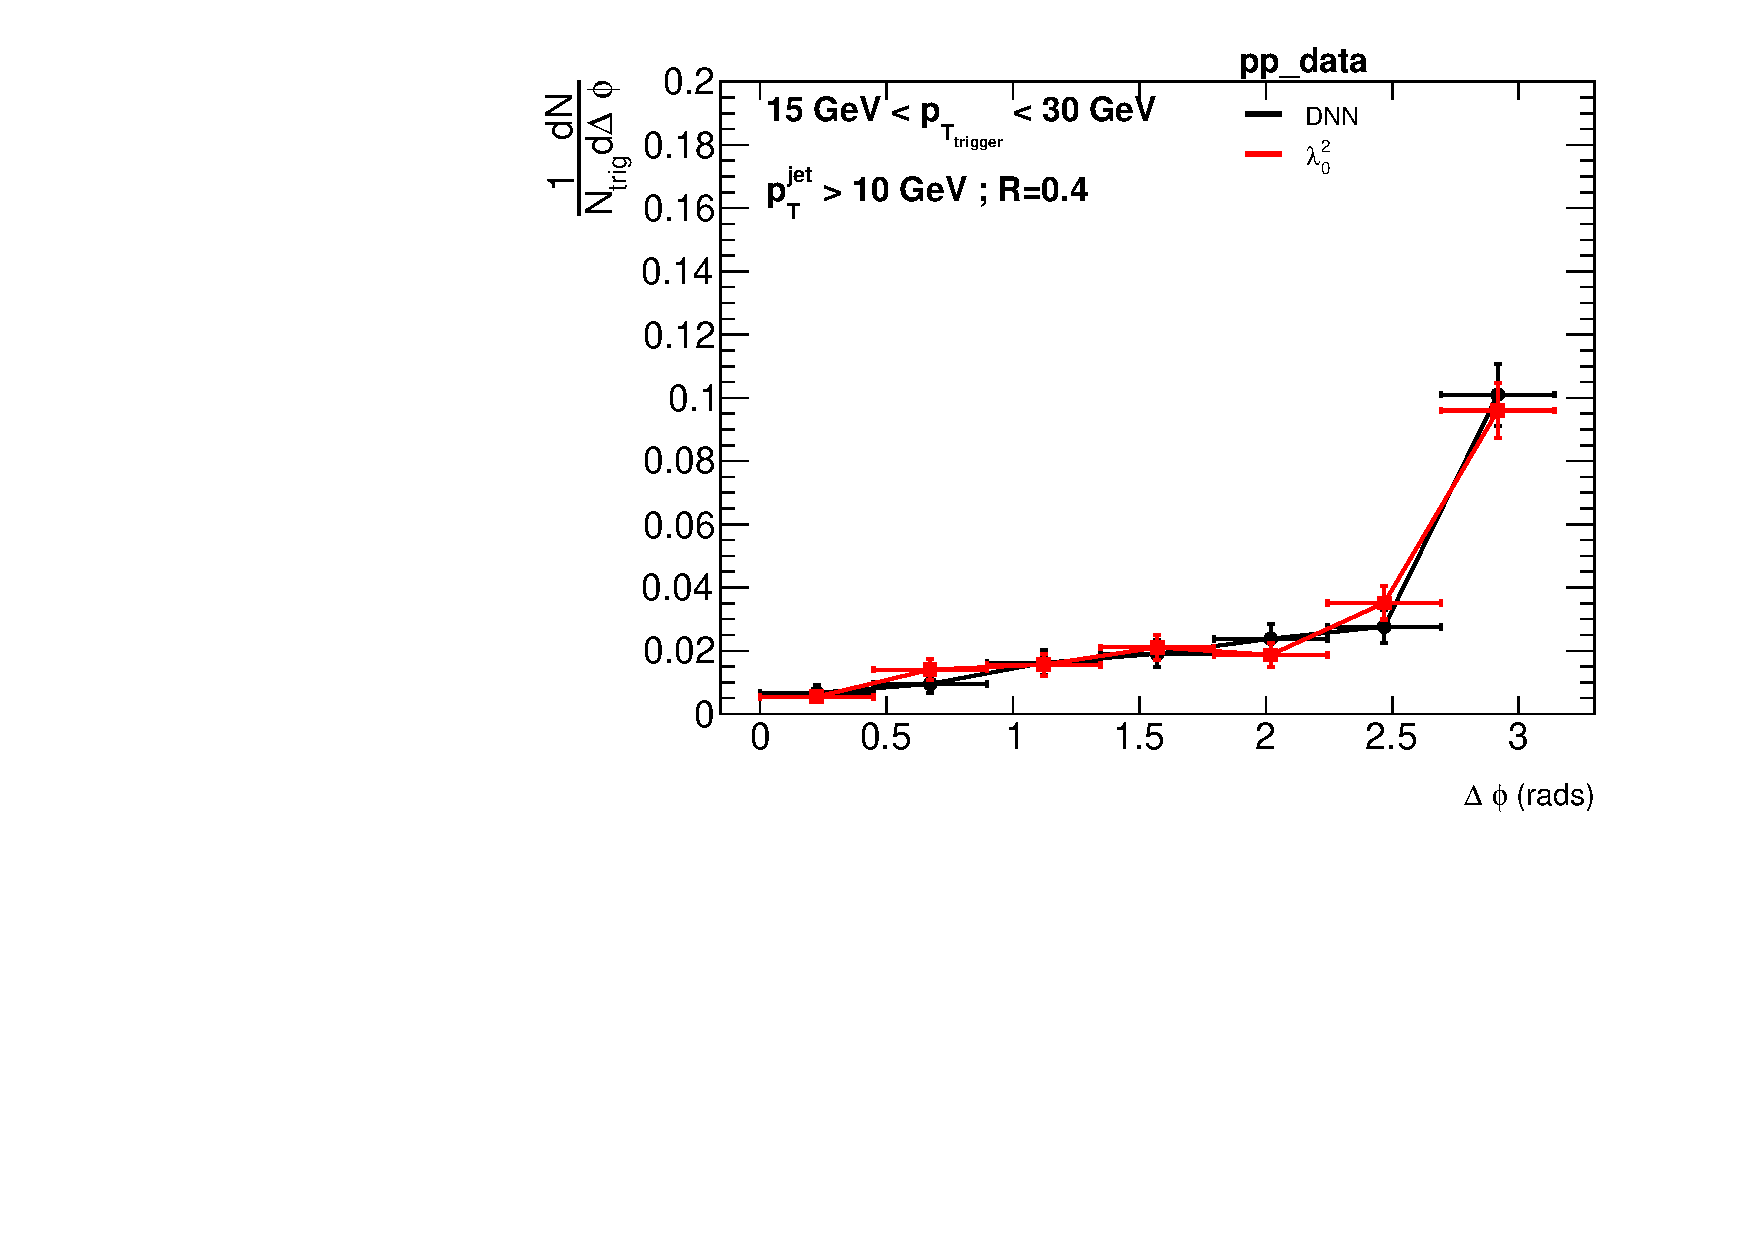
\includegraphics[width=0.49\textwidth]{GammaJet/sig_dPhipp_data_Comparison.pdf}
%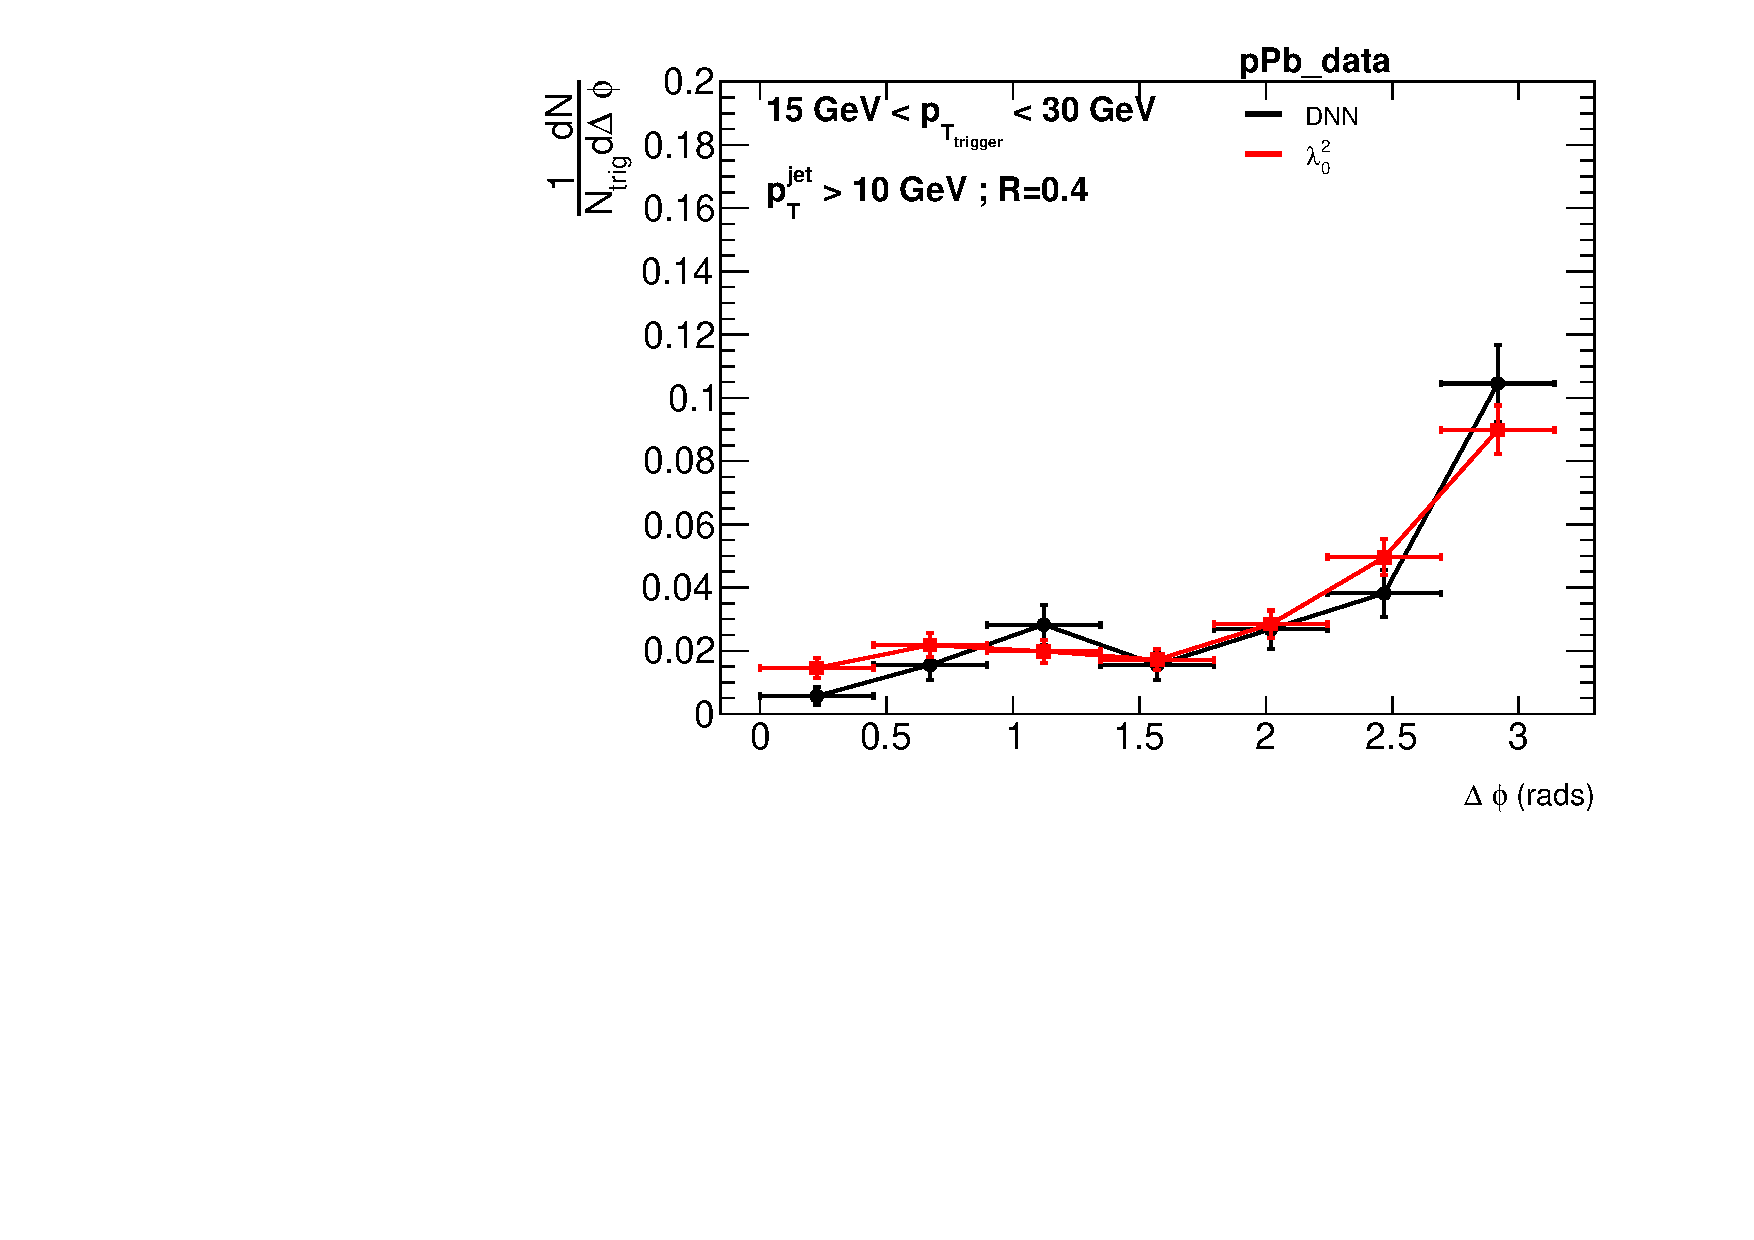
\includegraphics[width=0.49\textwidth]{GammaJet/sig_dPhipPb_data_Comparison.pdf}\\
%\includegraphics[width=0.49\textwidth]{GammaJet/hadj_dPhipp_data_Comparison.pdf}
%\includegraphics[width=0.49\textwidth]{GammaJet/hadj_dPhipPb_data_Comparison.pdf}
%\caption{Azimuthal separation $\Delta\phi$ for pp (left) and p-Pb data (right). The upper row shows the distributions for $\gammaiso$ candidates (signal region) and the bottom row for $\gammaiso$ with $\ydecay$ subtracted using Equation $\ref{eq:32}$. The error bar represents statistical uncertainty only.}
%\label{fig:gammajetdphi}
%\end{figure}

%\begin{figure}[h]
%\center
%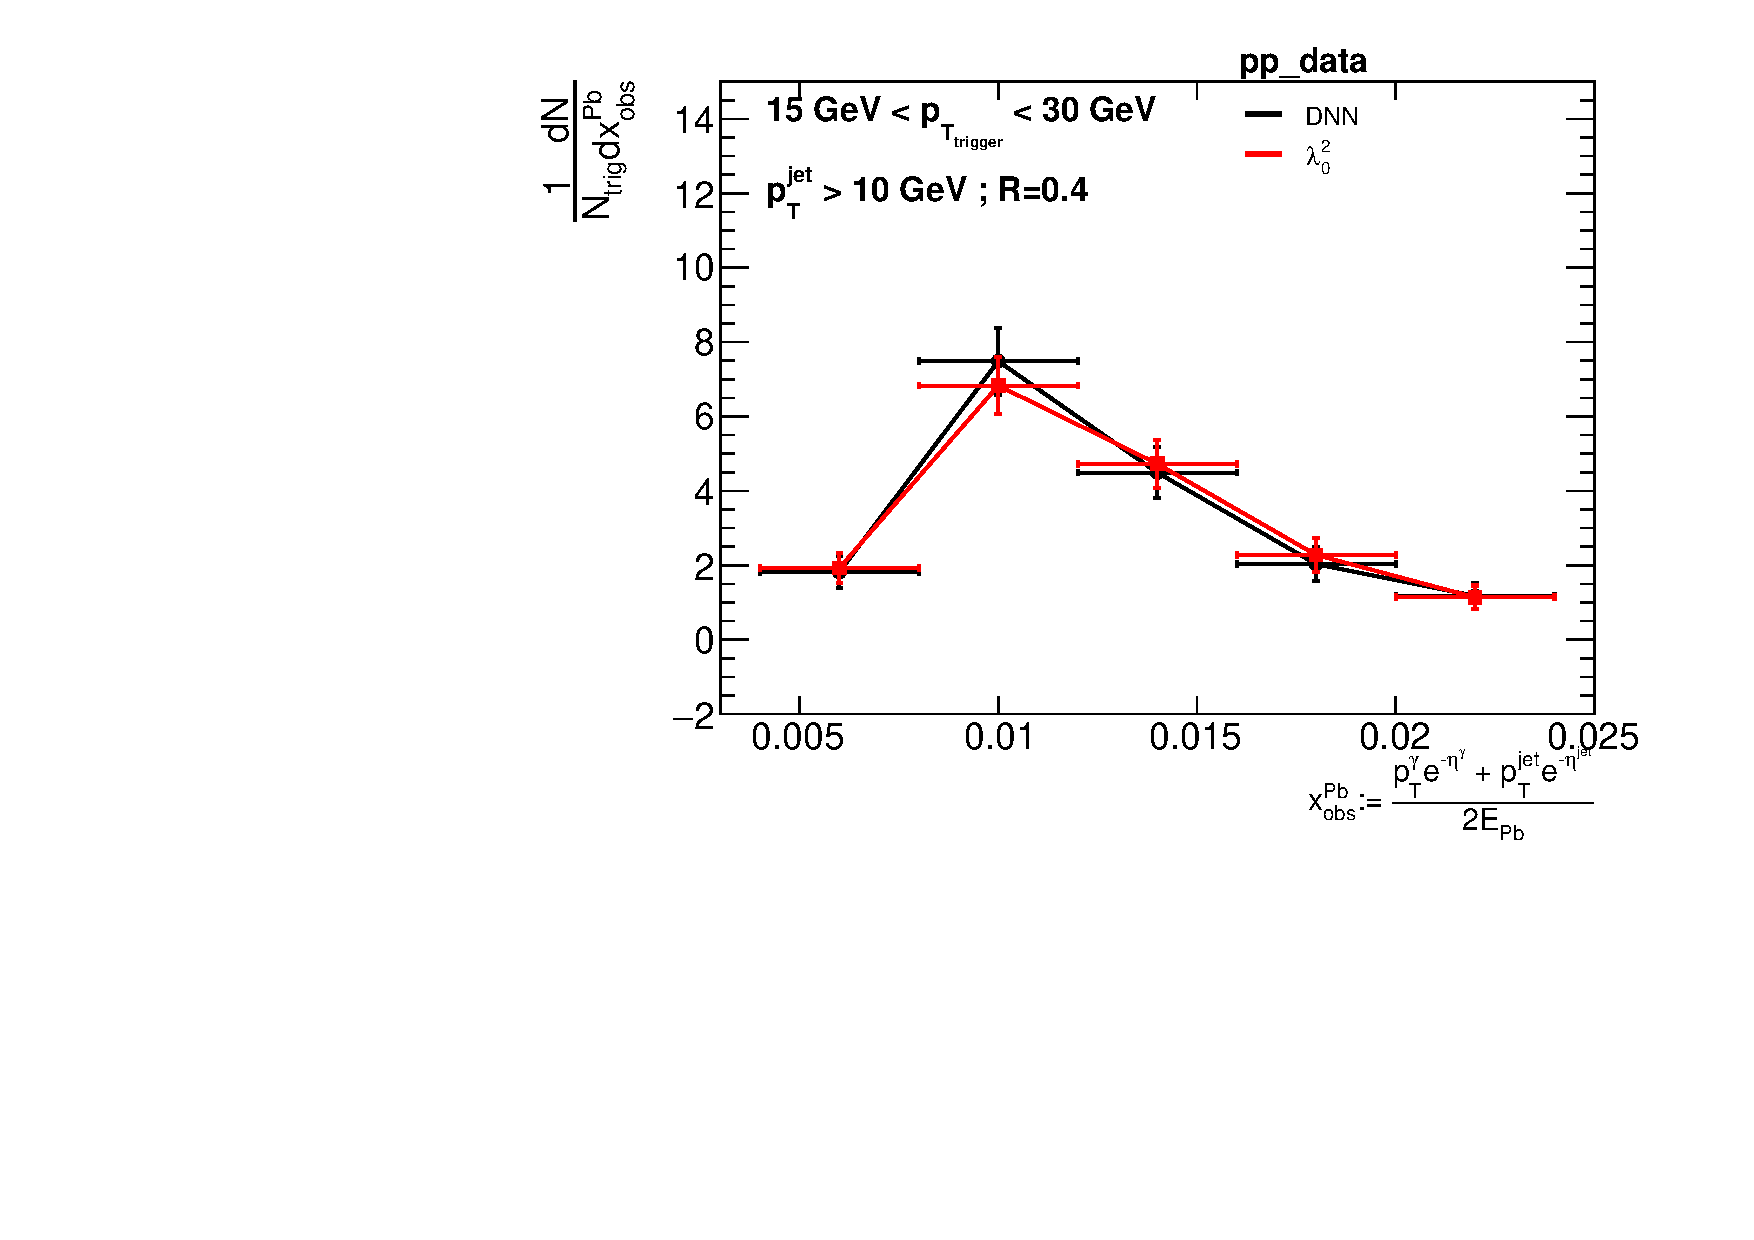
\includegraphics[width=0.49\textwidth]{GammaJet/sig_XobsPbpp_data_Comparison.pdf}
%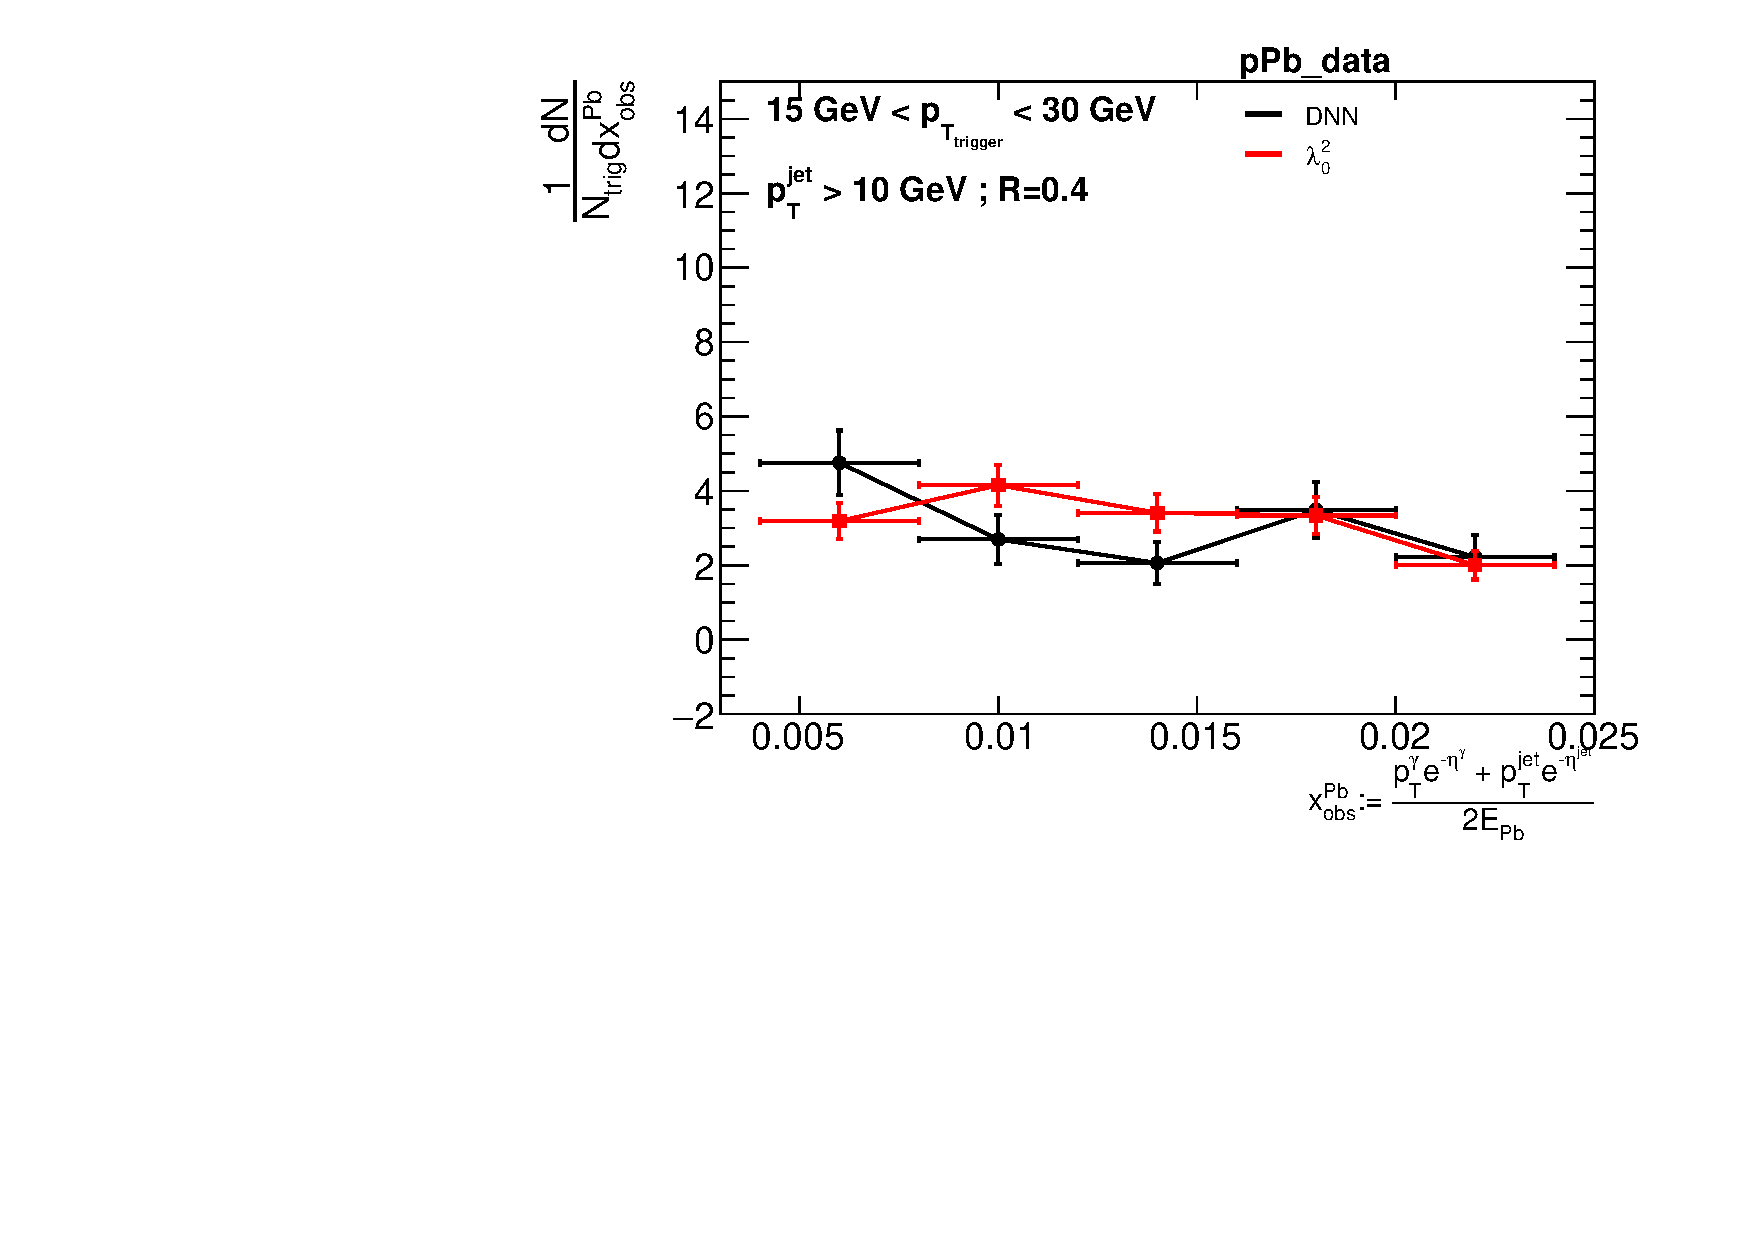
\includegraphics[width=0.49\textwidth]{GammaJet/sig_XobsPbpPb_data_Comparison.pdf}\\
%\includegraphics[width=0.49\textwidth]{GammaJet/hadj_XobsPbpp_data_Comparison.pdf}
%\includegraphics[width=0.49\textwidth]{GammaJet/hadj_XobsPbpPb_data_Comparison.pdf}
%\caption{$x_{obs}^{Pb}$ for pp (left) and p-Pb data (right). The upper row shows the distributions for $\gammaiso$ candidates (signal region) and the bottom row for $\gammaiso$ with $\ydecay$ subtracted using Equation $\ref{eq:32}$. The error bar represents statistical uncertainty only.}
%\label{fig:gammajetXobsPb}
%\end{figure}

%\begin{figure}[h]
%\center
%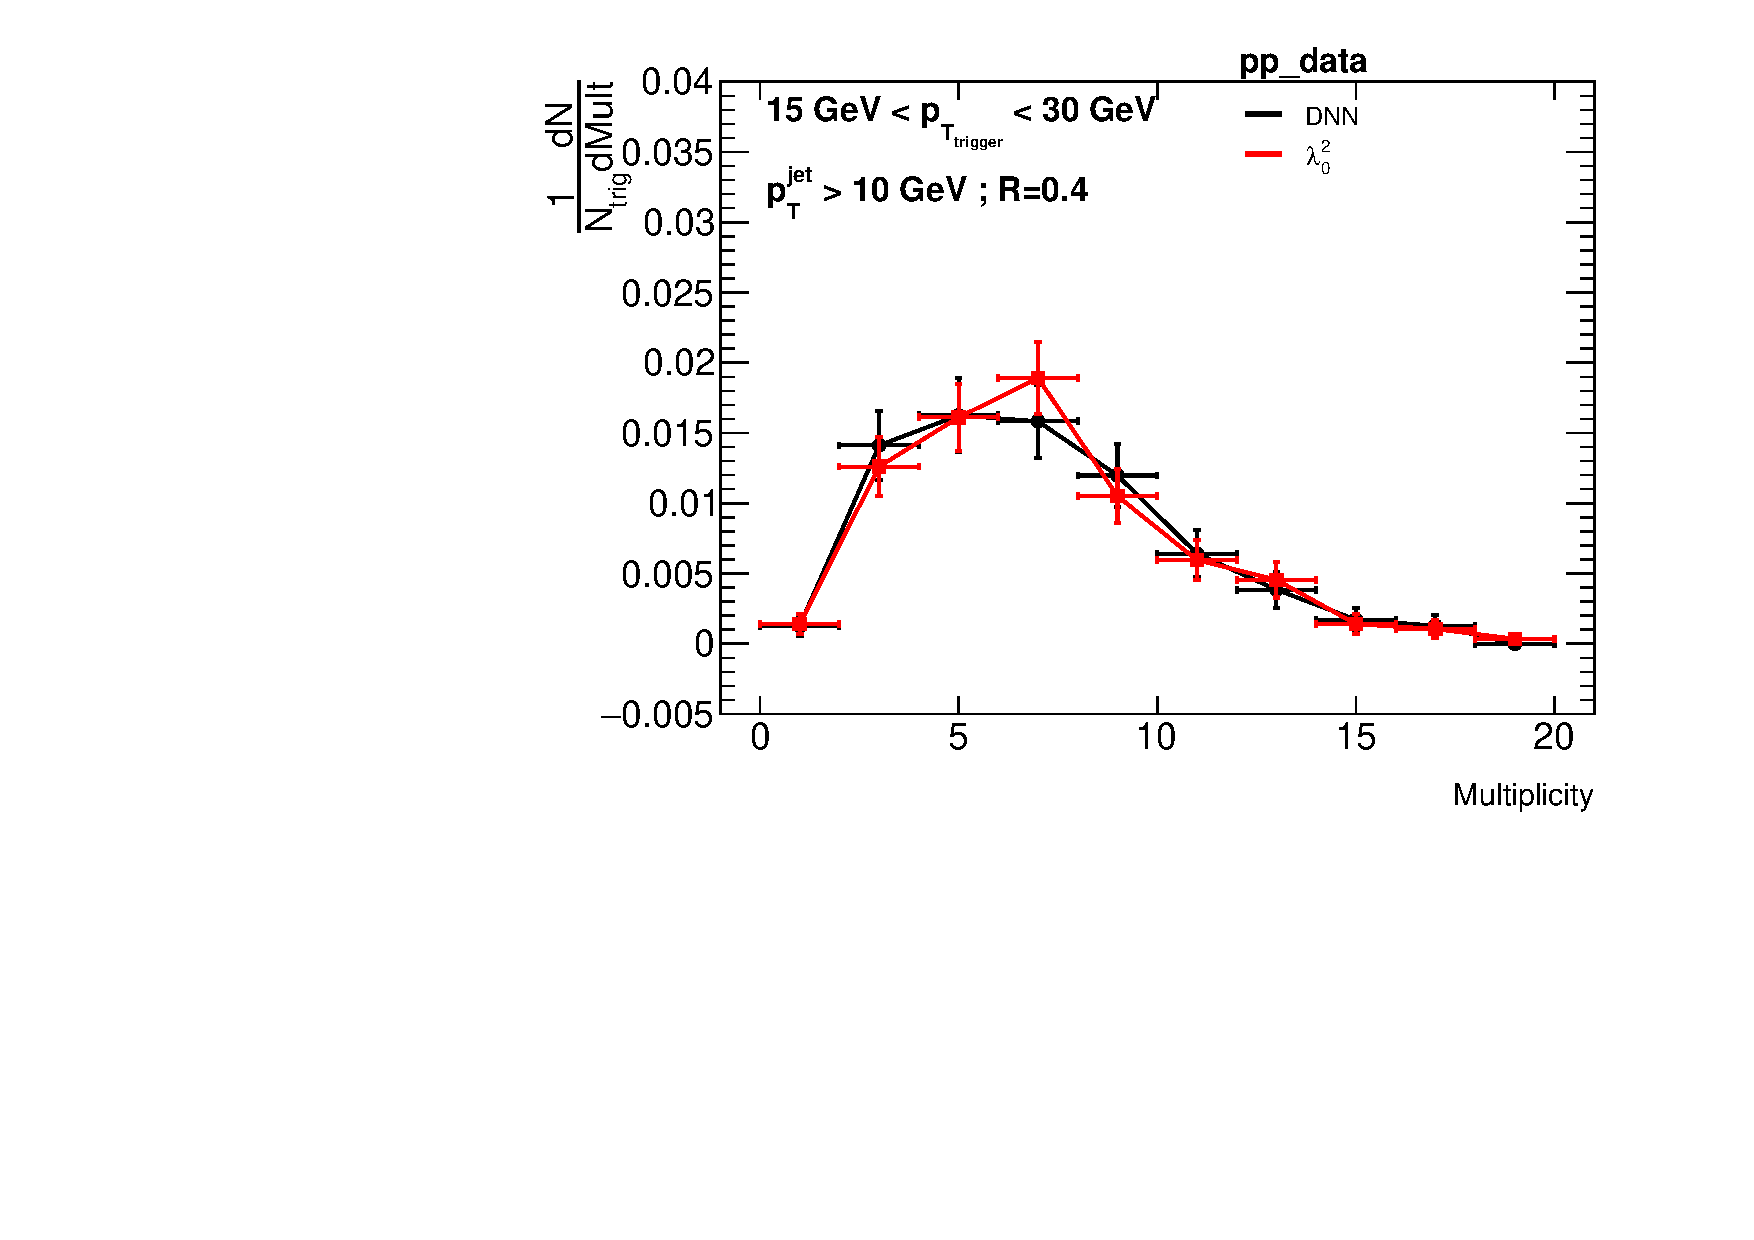
\includegraphics[width=0.49\textwidth]{GammaJet/sig_Multiplicitypp_data_Comparison.pdf}
%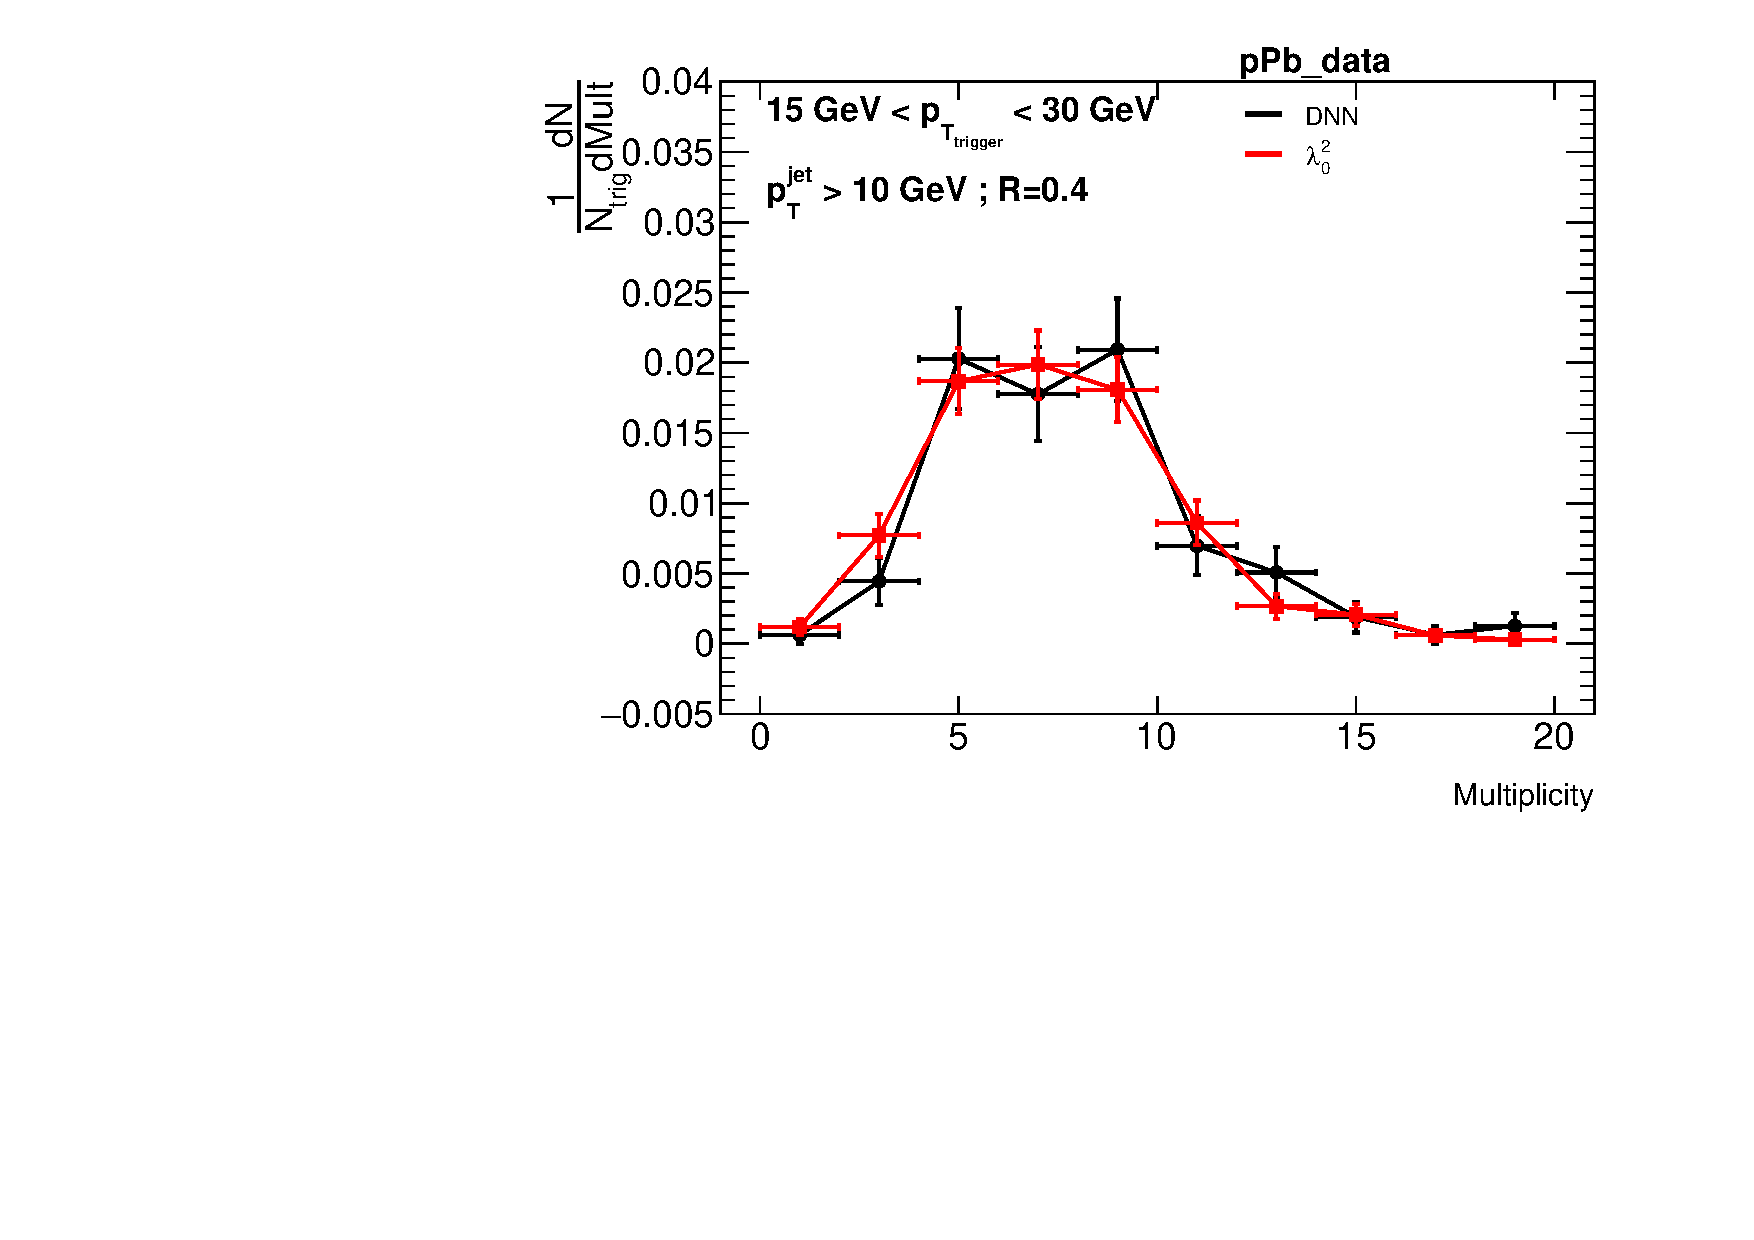
\includegraphics[width=0.49\textwidth]{GammaJet/sig_MultiplicitypPb_data_Comparison.pdf}\\
%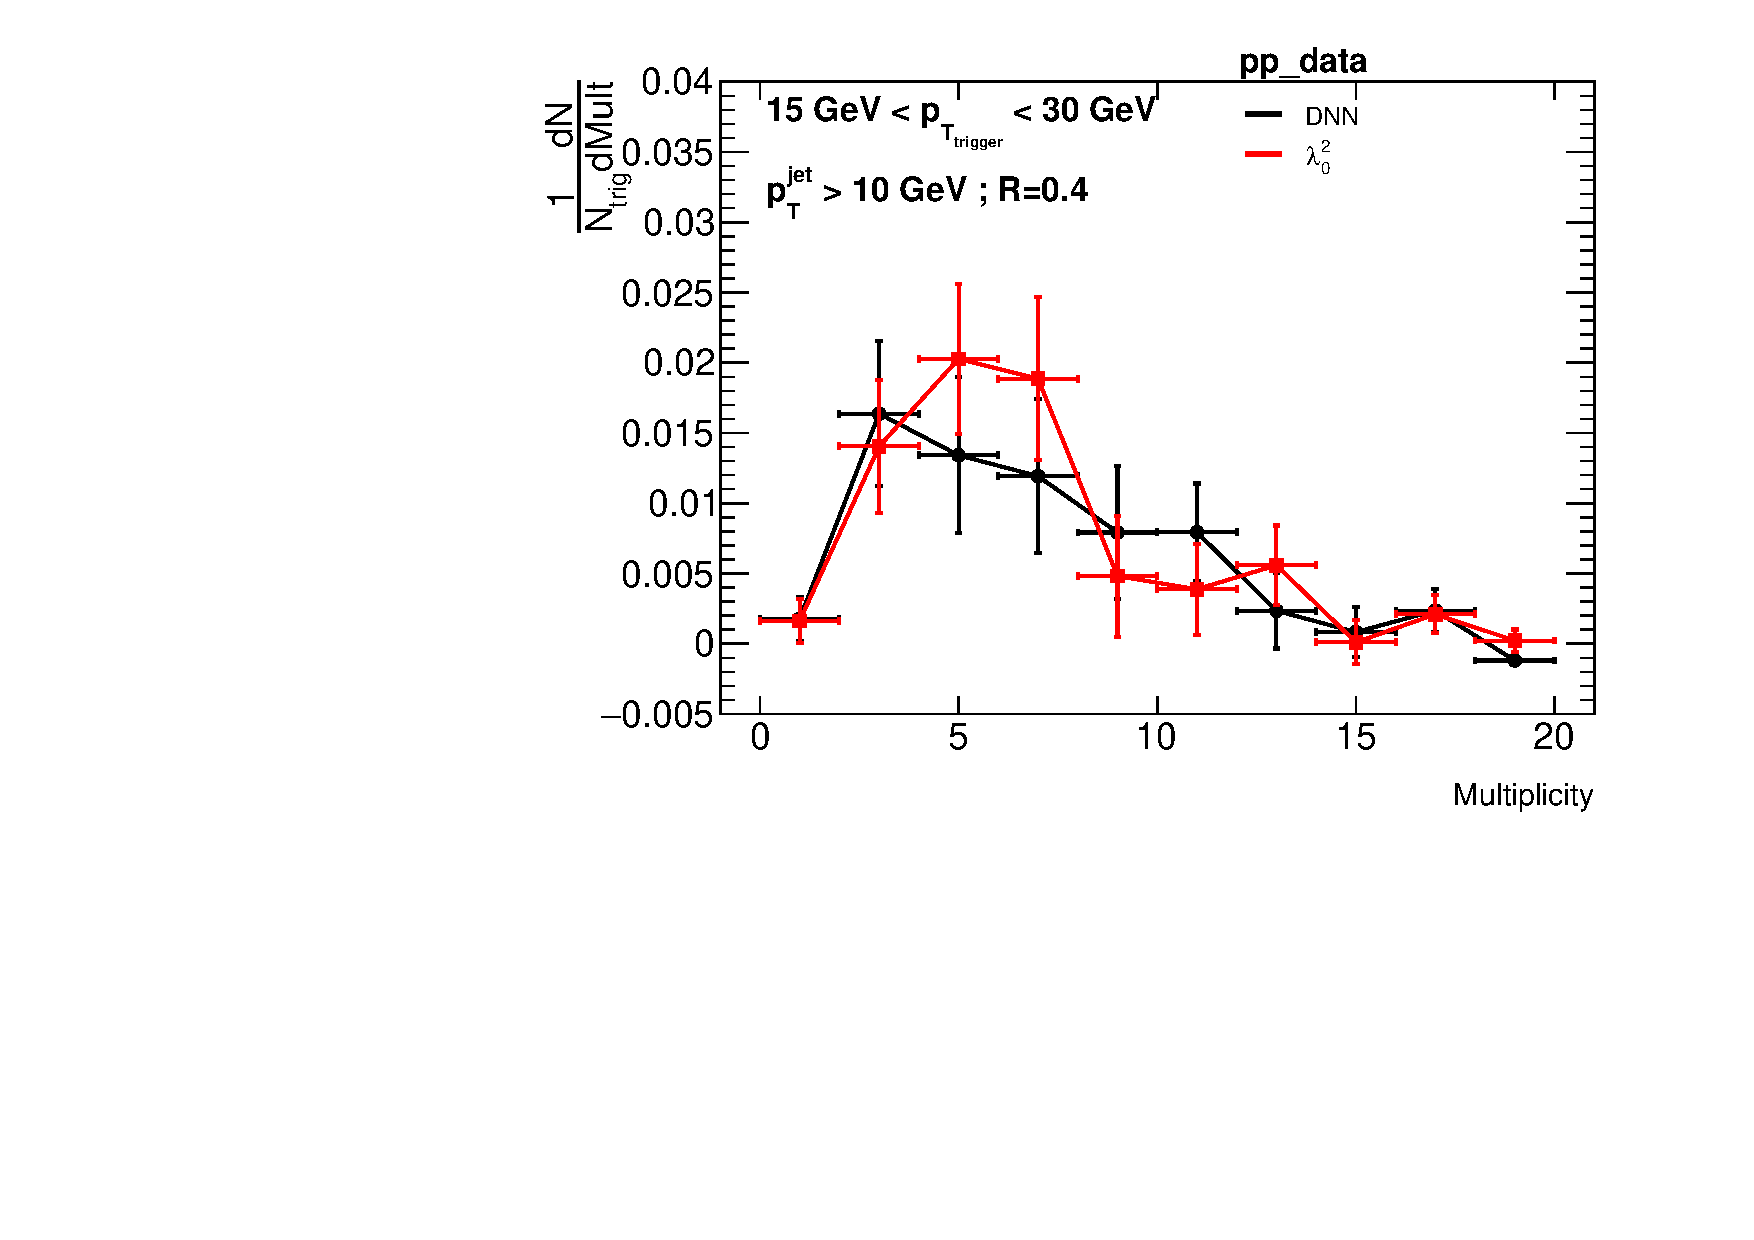
\includegraphics[width=0.49\textwidth]{GammaJet/hadj_Multiplicitypp_data_Comparison.pdf}
%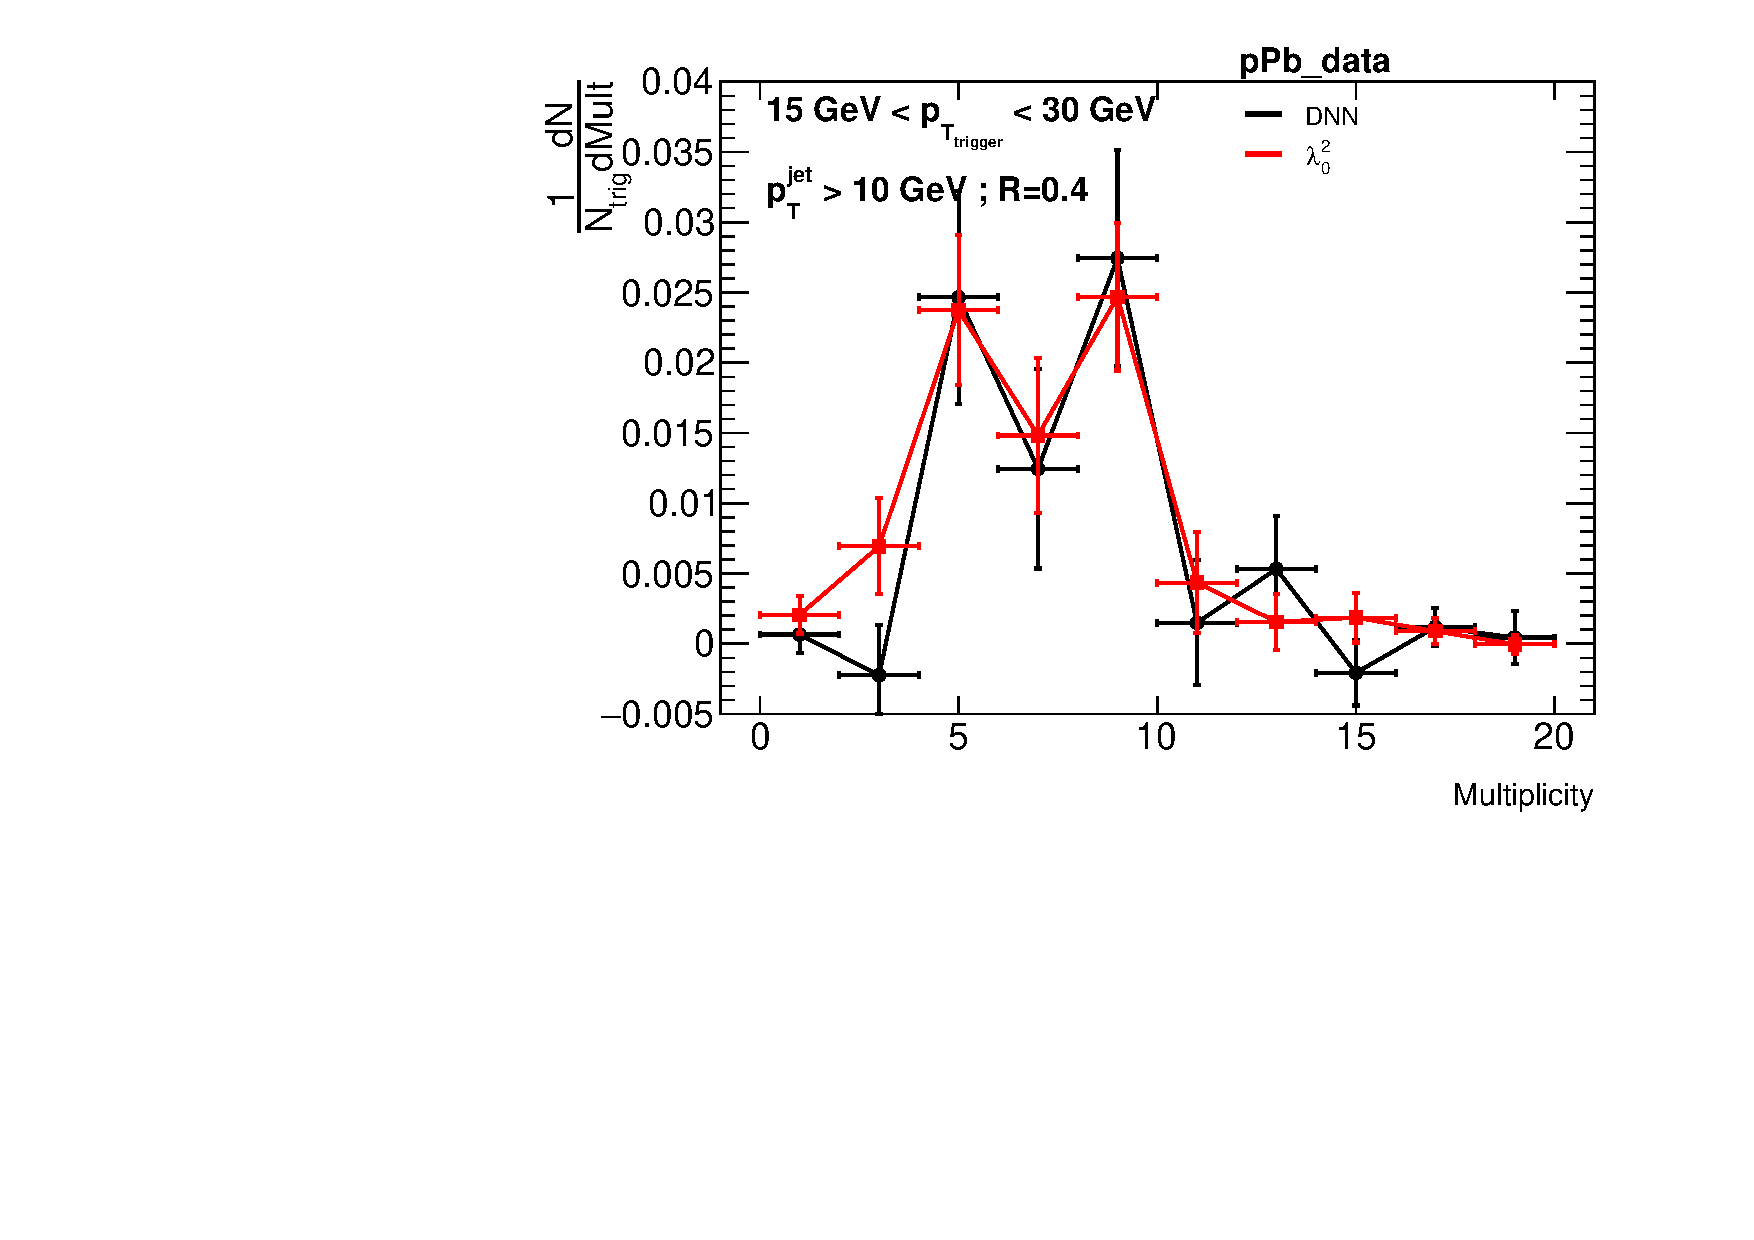
\includegraphics[width=0.49\textwidth]{GammaJet/hadj_MultiplicitypPb_data_Comparison.pdf}
%\caption{Multiplicity for pp (left) and p-Pb data (right). The upper row shows the distributions for $\gammaiso$ candidates (signal region) and the bottom row for $\gammaiso$ with $\ydecay$ subtracted using Equation $\ref{eq:32}$. The error bar represents statistical uncertainty only.}
%\label{fig:gammajetMultiplicity}
%\end{figure}

%\begin{figure}[h]
%\center
%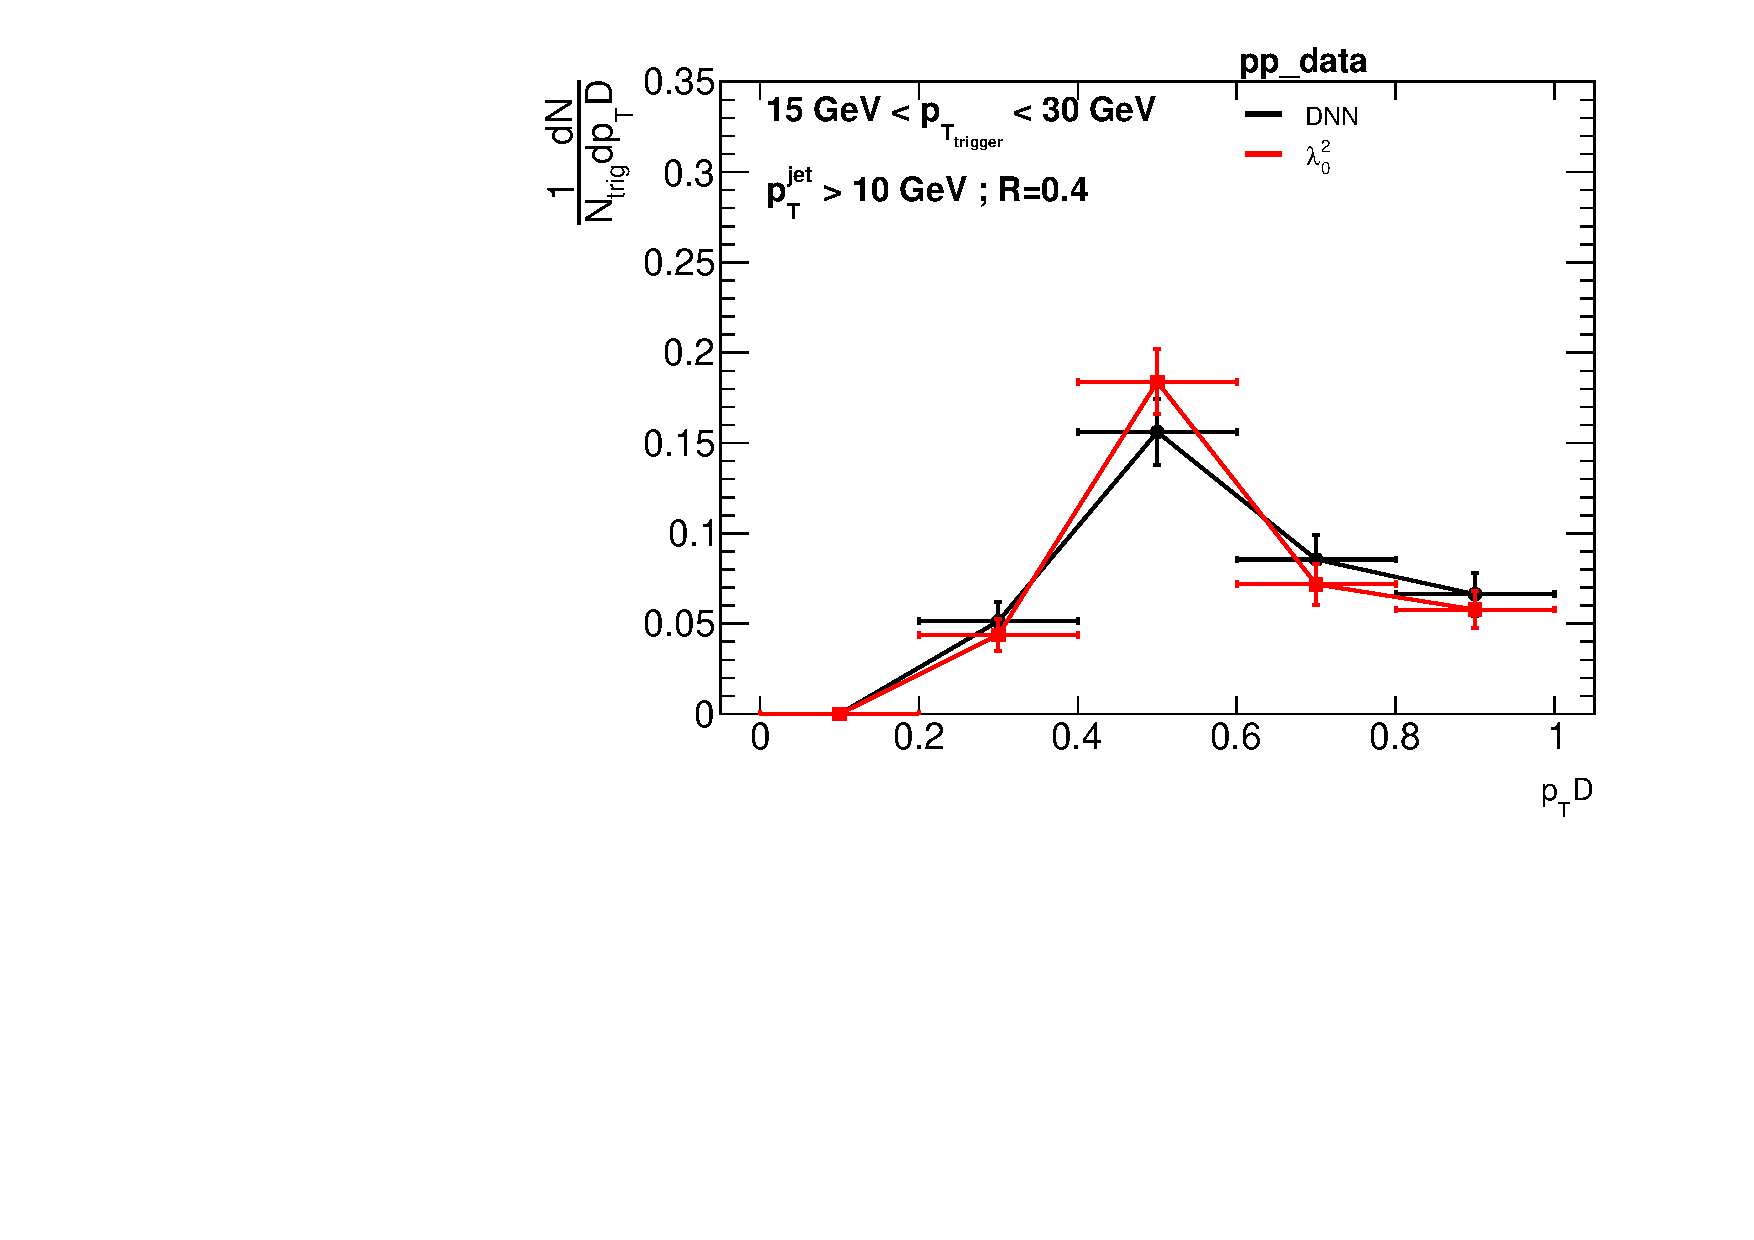
\includegraphics[width=0.49\textwidth]{GammaJet/sig_pTDpp_data_Comparison.pdf}
%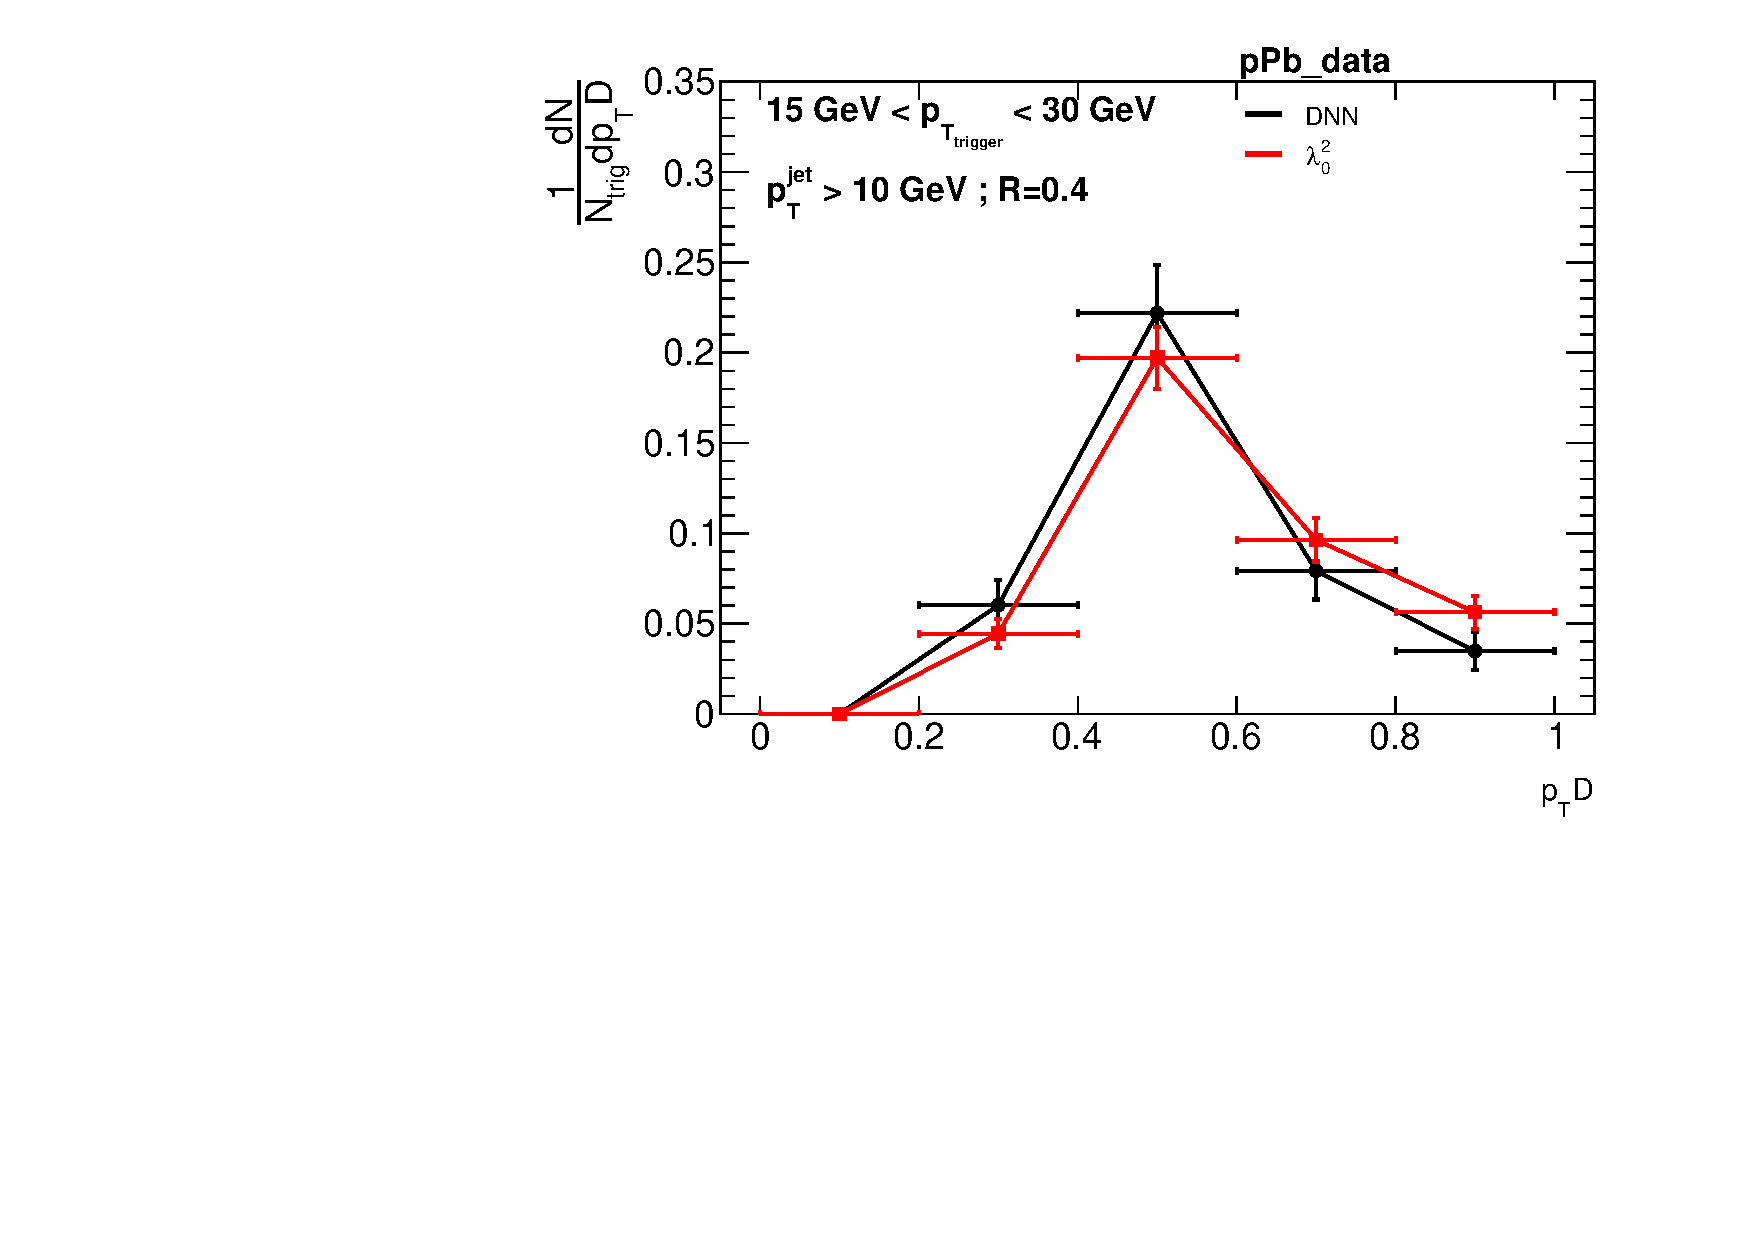
\includegraphics[width=0.49\textwidth]{GammaJet/sig_pTDpPb_data_Comparison.pdf}\\
%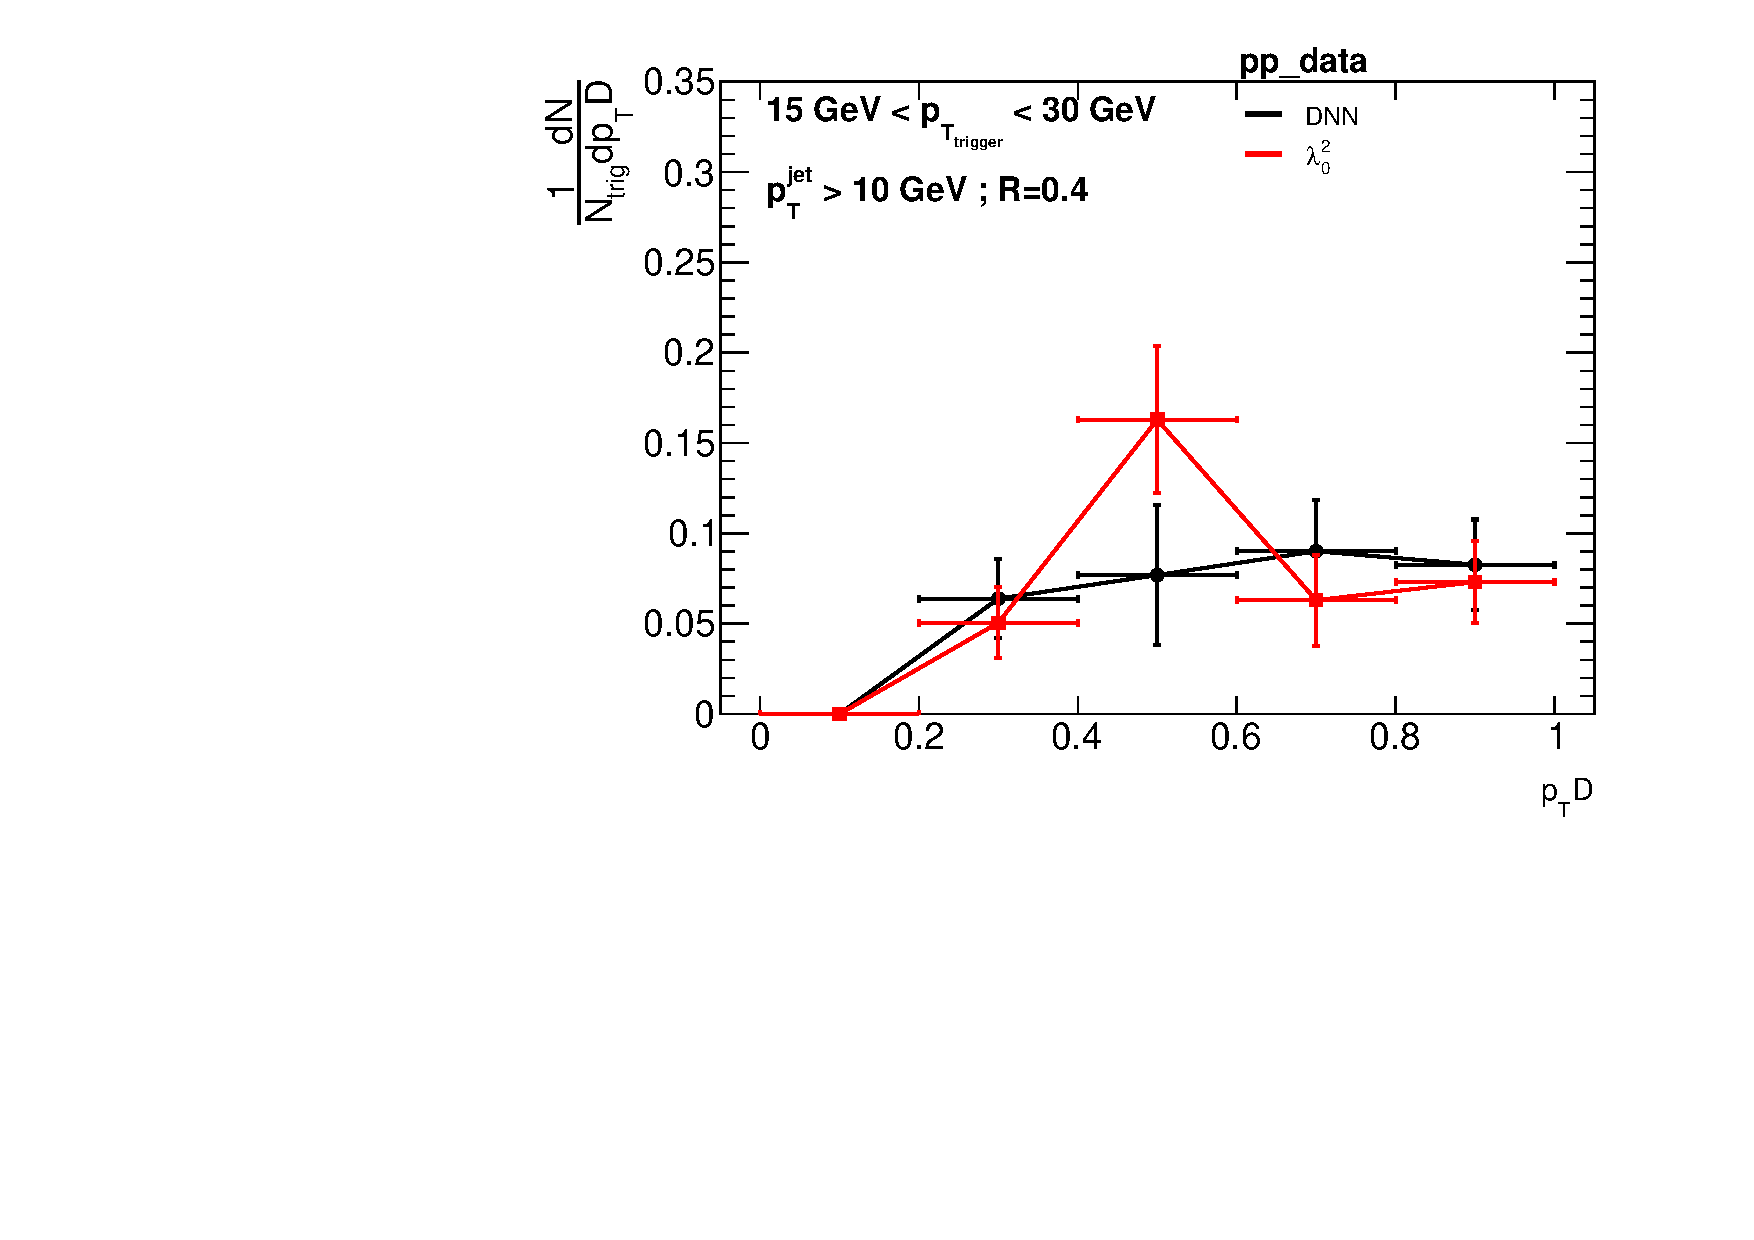
\includegraphics[width=0.49\textwidth]{GammaJet/hadj_pTDpp_data_Comparison.pdf}
%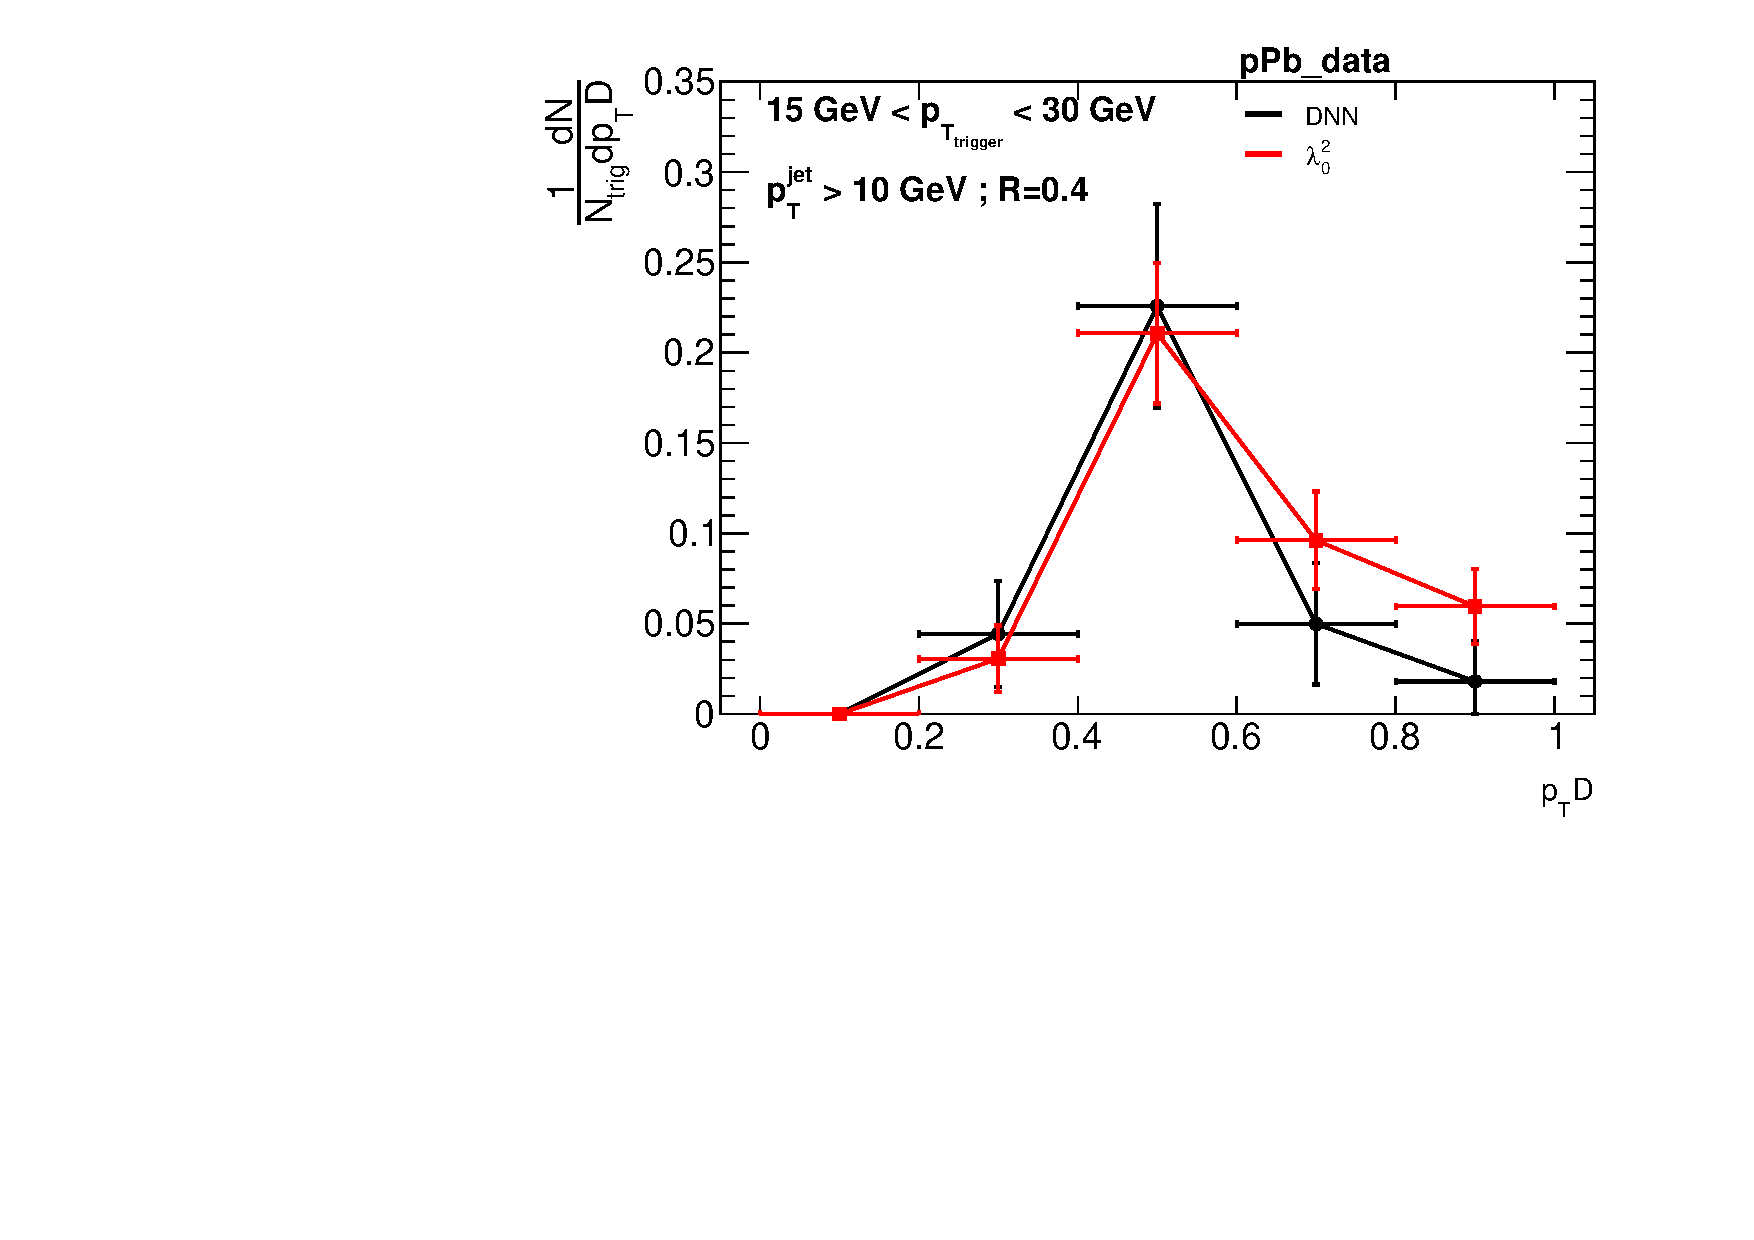
\includegraphics[width=0.49\textwidth]{GammaJet/hadj_pTDpPb_data_Comparison.pdf}
%\caption{$p_{T}D$ for pp (left) and p-Pb data (right). The upper row shows the distributions for $\gammaiso$ candidates (signal region) and the bottom row for $\gammaiso$ with $\ydecay$ subtracted using Equation $\ref{eq:32}$. The error bar represents statistical uncertainty only.}
%\label{fig:gammajetpTD}
%\end{figure}

%\begin{figure}[h]
%\center
%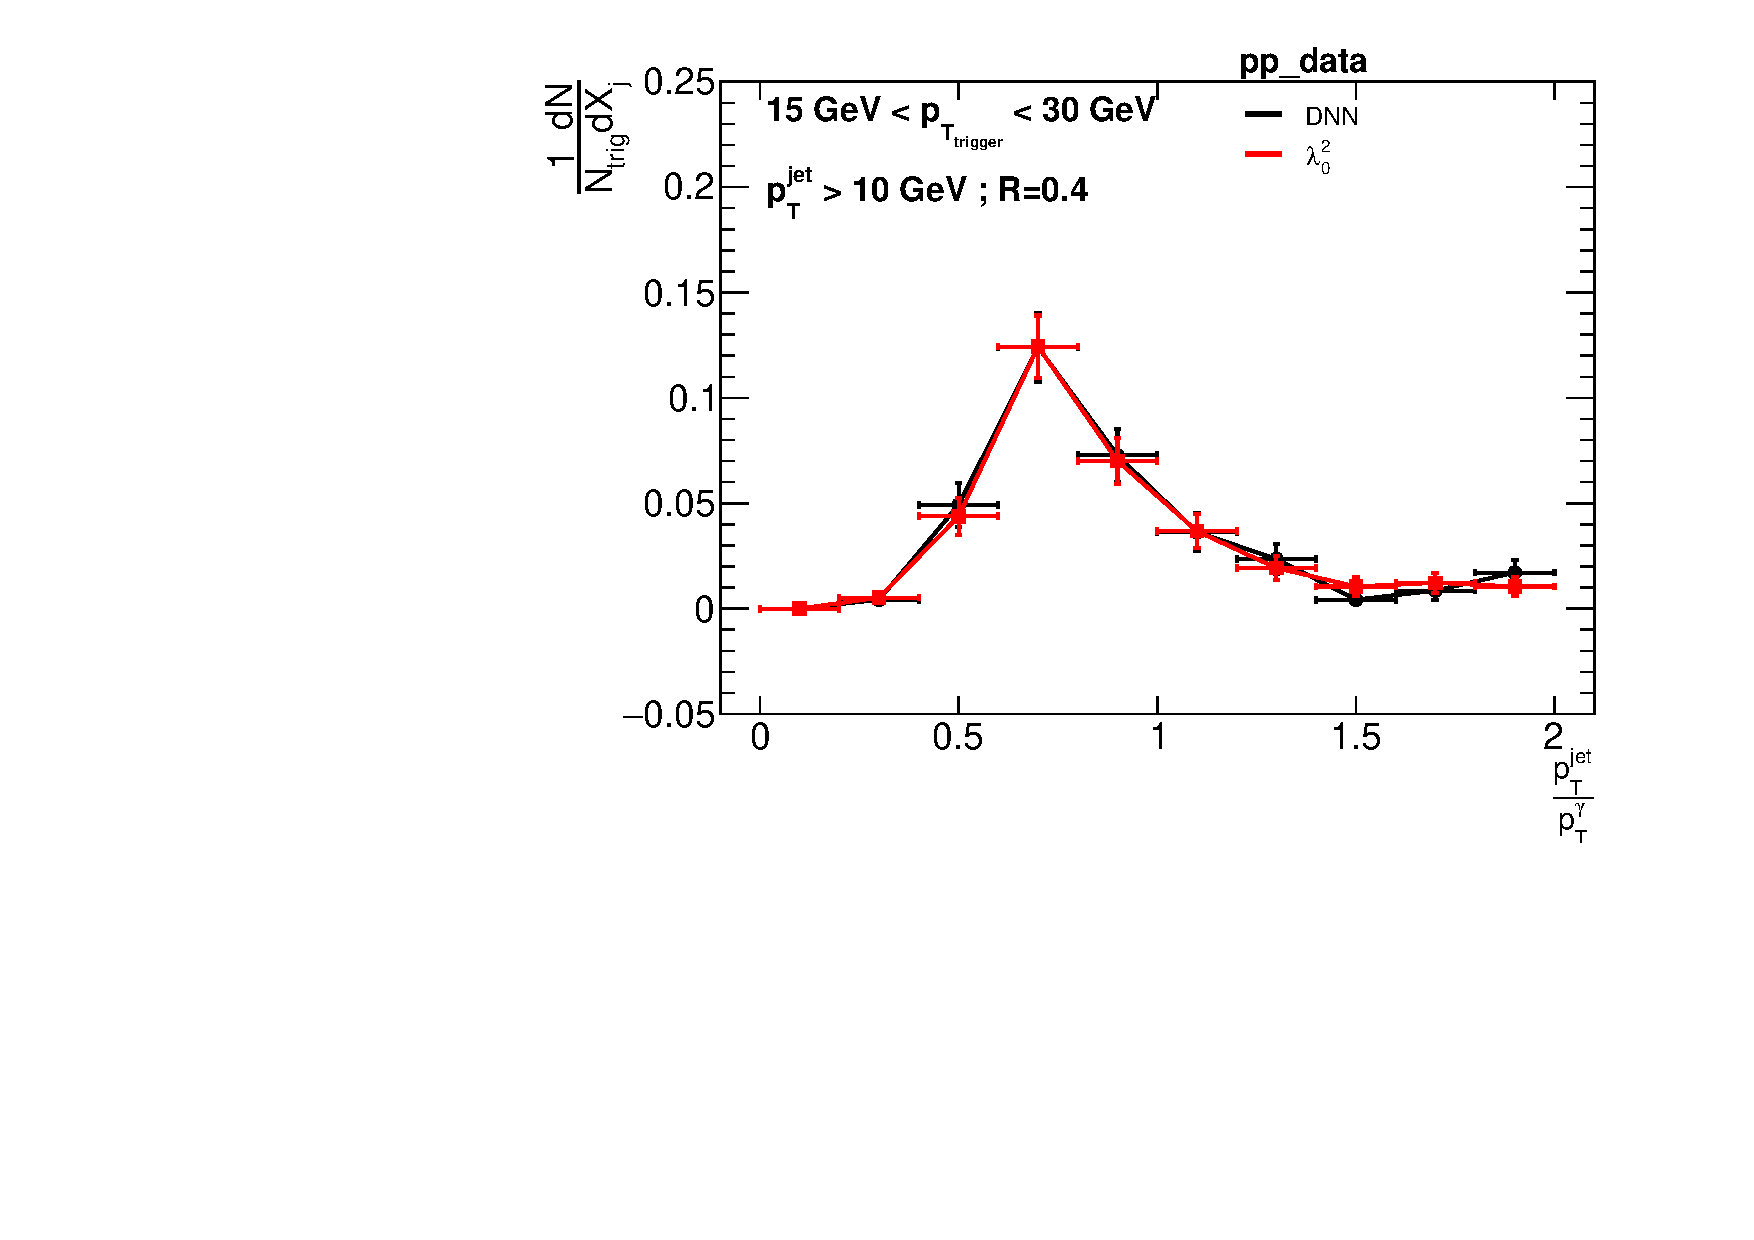
\includegraphics[width=0.49\textwidth]{GammaJet/sig_Xjpp_data_Comparison.pdf}
%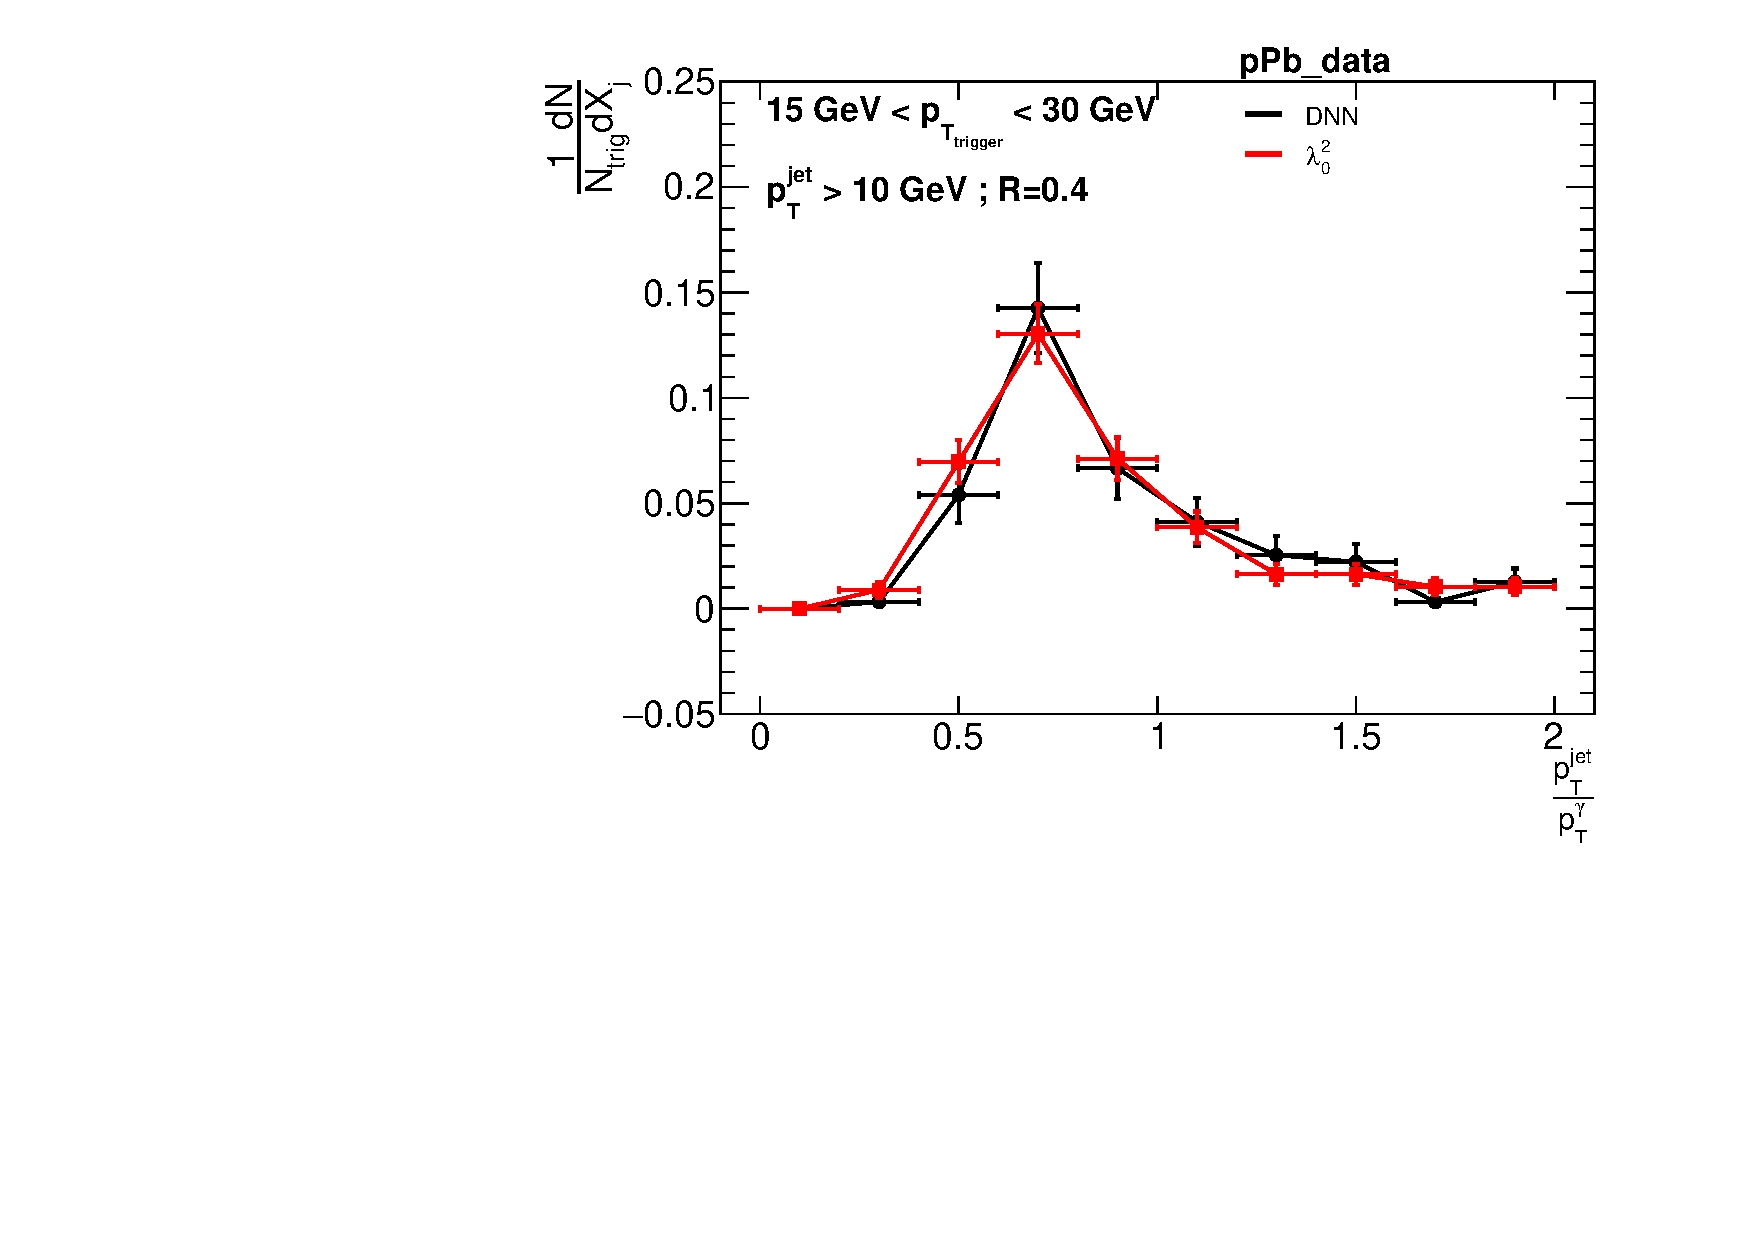
\includegraphics[width=0.49\textwidth]{GammaJet/sig_XjpPb_data_Comparison.pdf}\\
%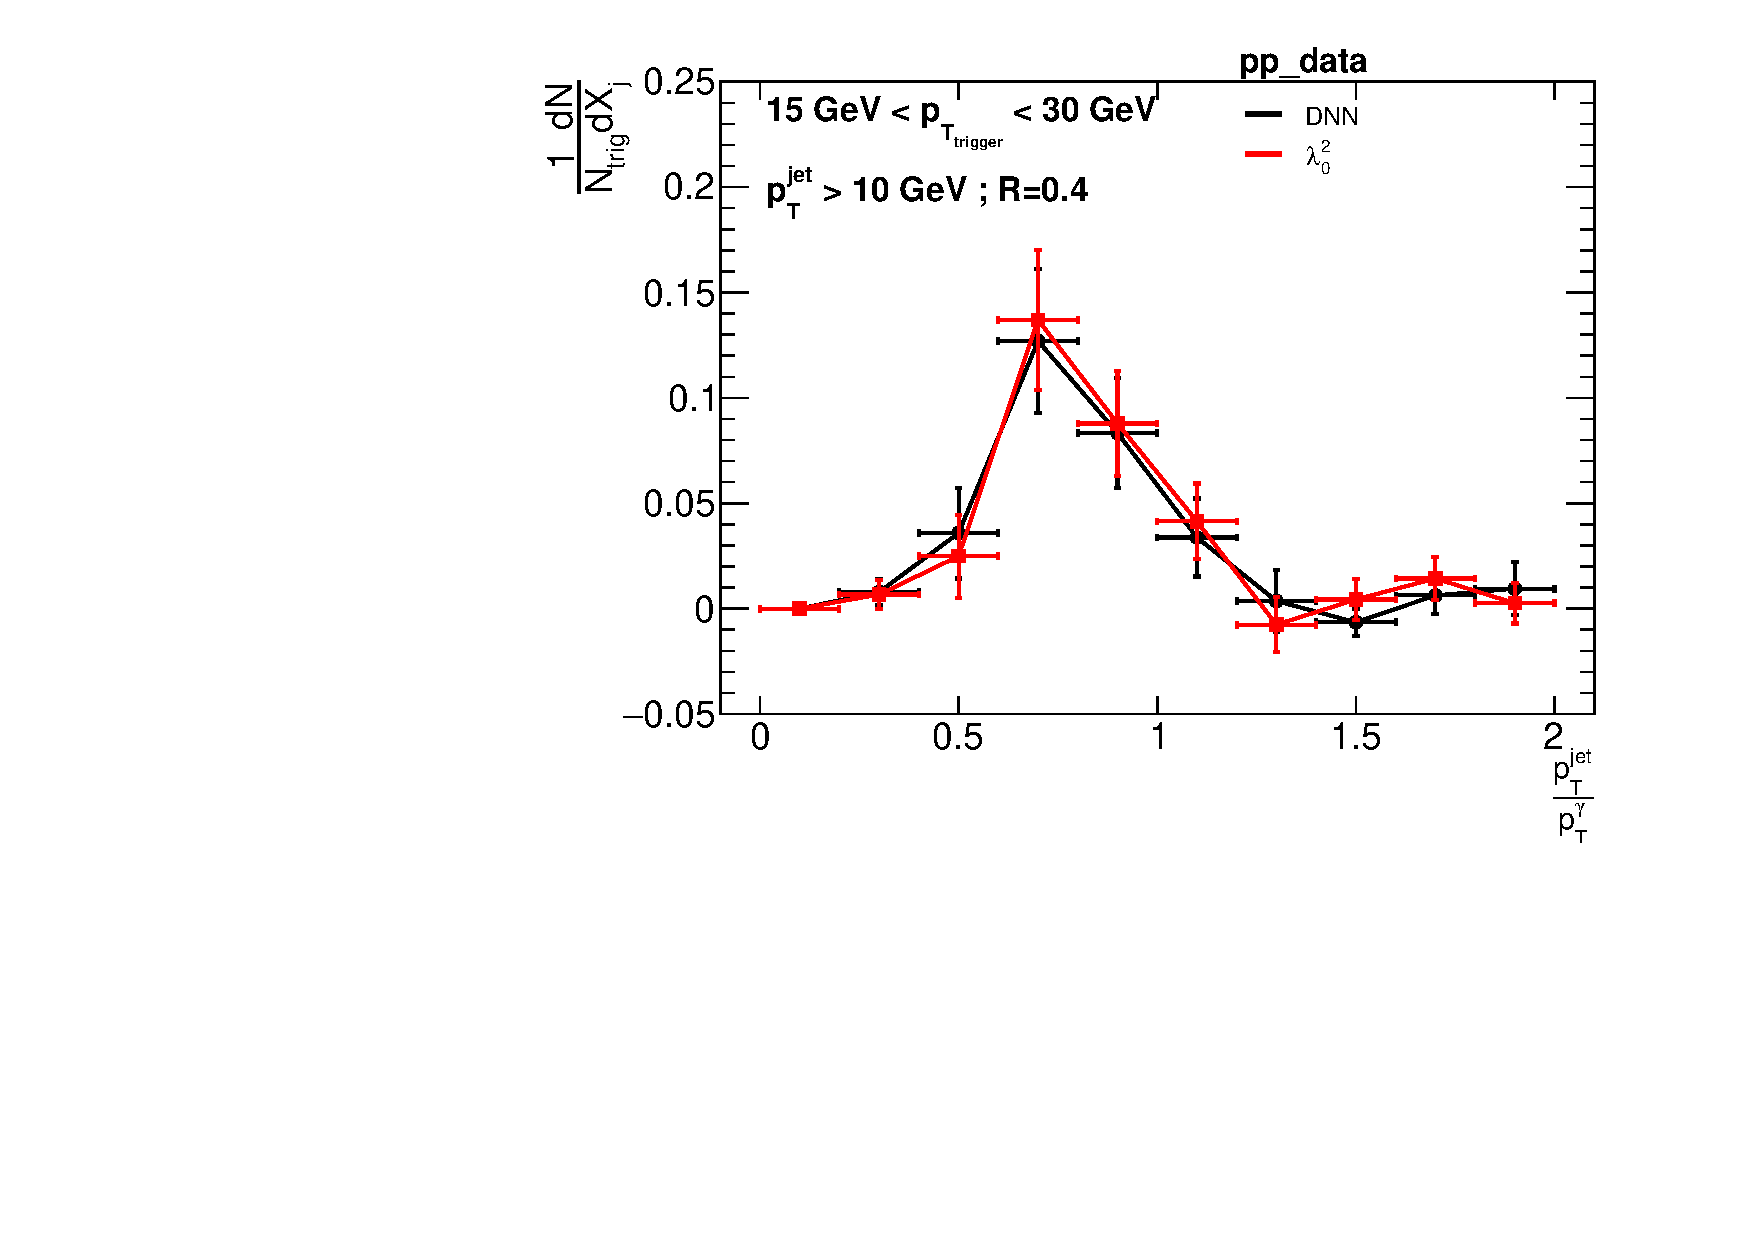
\includegraphics[width=0.49\textwidth]{GammaJet/hadj_Xjpp_data_Comparison.pdf}
%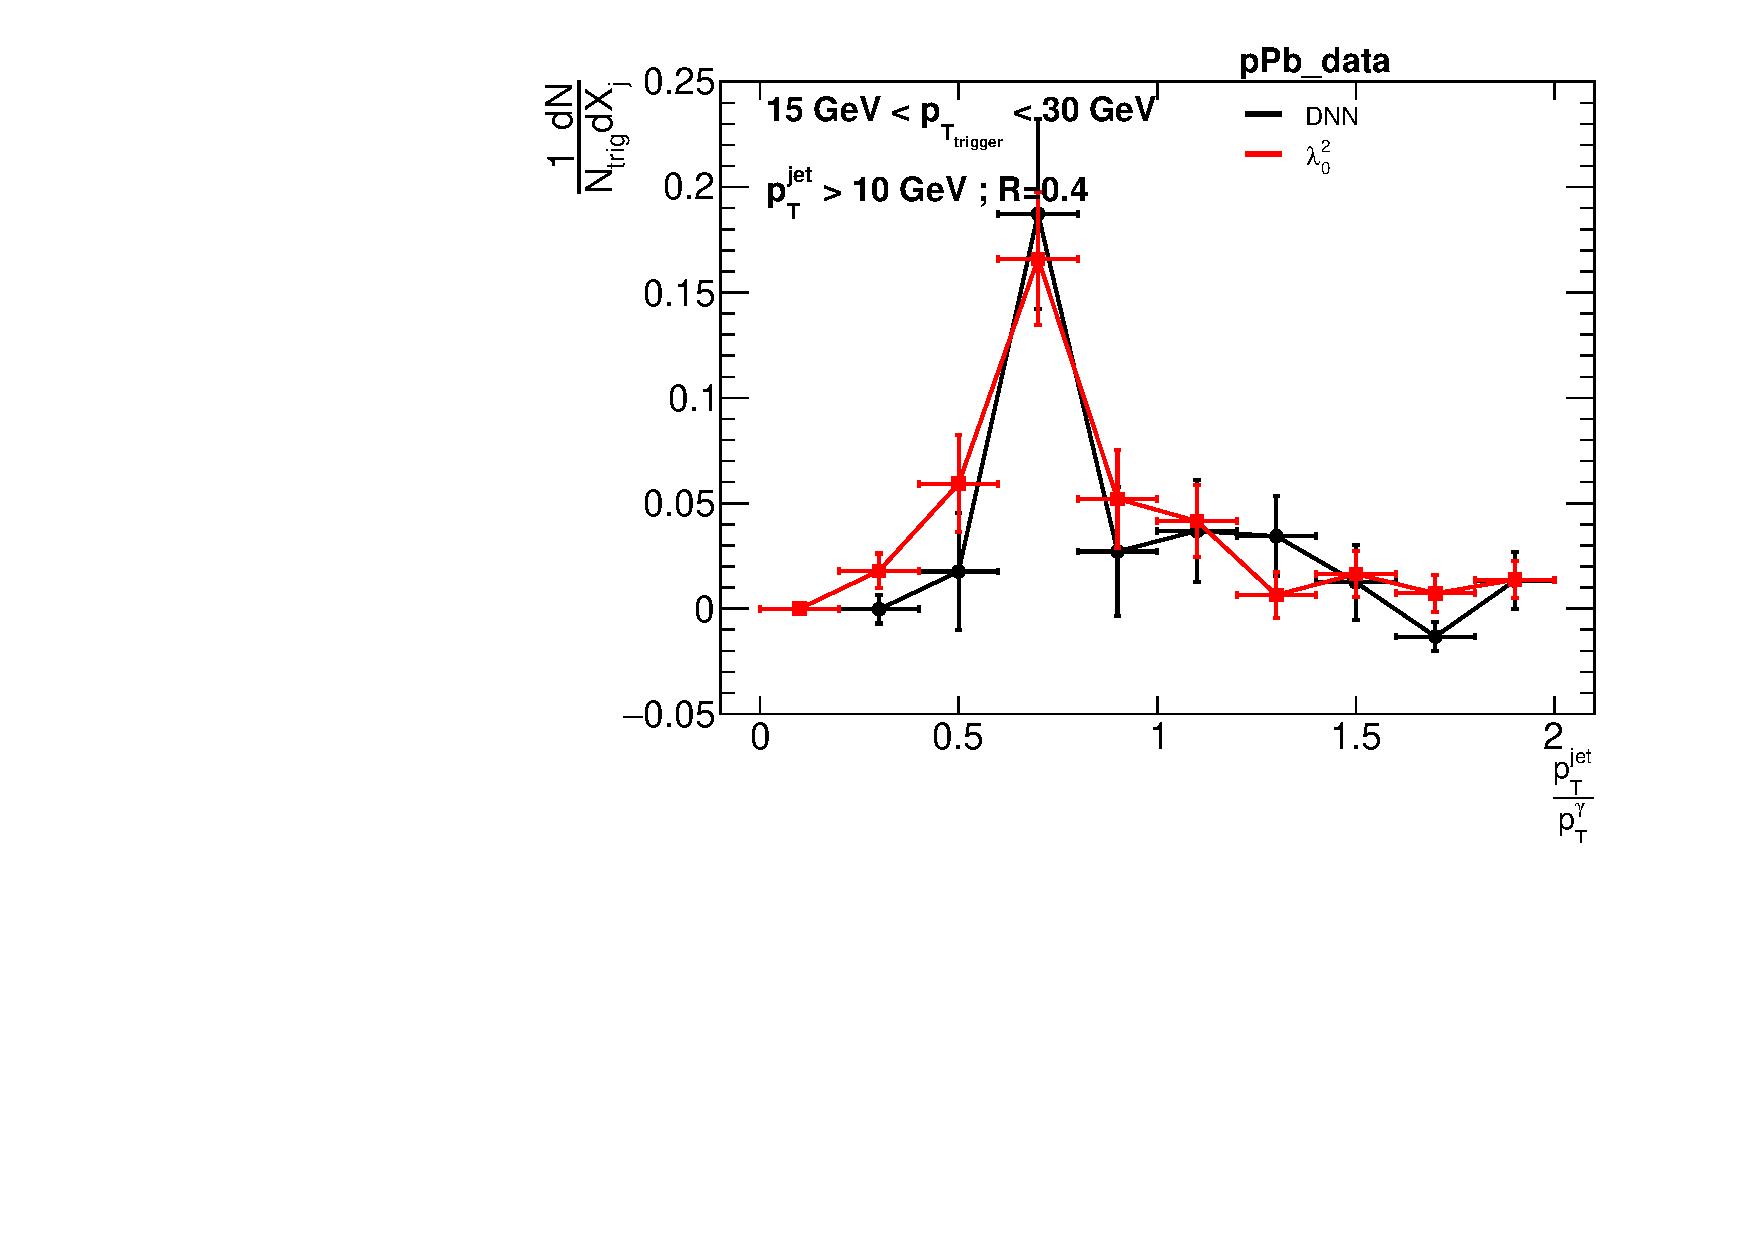
\includegraphics[width=0.49\textwidth]{GammaJet/hadj_XjpPb_data_Comparison.pdf}
%\caption{$X_j$ for pp (left) and p-Pb data (right). The upper row shows the distributions for $\gammaiso$ candidates (signal region) and the bottom row for $\gammaiso$ with $\ydecay$ subtracted using Equation $\ref{eq:32}$. The error bar represents statistical uncertainty only.}
%\label{fig:gammajetXj}
%\end{figure}

%Here, the azimuthal difference distribution shows a peak at $\Delta\phi =\pi$, as expected, and a tail that extends to large values. The results are compatible within uncertainties among different shower-shape selections. It is also very similar between pp and p-Pb data, which indicates that the tail towards larger values is not completely dominated by fake jets due to underlying-event fluctuations (that would be higher in p-Pb collisions). The distributions are also similar between the signal-region ($\gammaiso$ enriched) and the background region ($\ydecay$ enriched). 

%Figure~\ref{fig:dphiGammaIso} shows the distributions for $\gammaiso$ correlations, obtained using the measured purity and the 
%Equation~\ref{eq:FinalSubtraction}. The statistical uncertainty is higher in this case, as the purity statistical uncertainty has been propagated to this measurement. Note that there is a large overlap between the shower-shape selection so the statistical uncertainties shown here are highly correlated. The distributions are compatible among shower-shape selections and between pp and p-Pb data. 

%\begin{figure}
%\center
%\includegraphics[width=0.49\textwidth]{GammaJet/hadj_dPhipp_data_Comparison.pdf}
%\includegraphics[width=0.49\textwidth]{GammaJet/hadj_dPhipPb_data_Comparison.pdf}
%\caption{Azimuthal separation $\Delta\phi$ between $\gammaiso$ and jets for pp (left) and p-Pb data (right). The $\ydecay$ contribution is subtracted following Equation \ref{eq:FinalSubtraction}. The error bar represents the combination of statistical uncertainty in the data and the statistical uncertainty in the purity measurement. }
%\label{fig:dphiGammaIso}
%\end{figure}
%\FloatBarrier

%\subsubsection{Distributions from photon+jet simulation}

%Figure~\ref{fig:dPhiMC} shows the distribution from photon+jet simulation at both the reconstructed level and truth level. 
%The simulated data is treated in the same way as the data (clusters and jet selections), except that we make no purity correction as in Equation~\ref{eq:FinalSubtraction}, for obvious reasons. The normalization of the simulated correlation distribution is the same as in data, i.e. per-photon. The simulation does not describe the shape of the $\Delta\phi$ distribution well. This is likely due to the fact that \textsc{Pythia} is a leading-order generator, and therefore neglects configurations between $\gammaiso$ + multijets that populate the large $\Delta\phi$ tails. 

%\begin{figure}[h]
%\center
%\includegraphics[width=0.49\textwidth]%{GammaJet/hSR_dPhi17g6a1_data_Comparison.pdf}
%\includegraphics[width=0.49\textwidth]{GammaJet/hSR_dPhi17g6a1_truths_Comparison.pdf}
%\caption{$\Delta \phi$ distribution for Gamma-jet simulation at reconstructed (left) and particle level (right) . The error bar represents statistical uncertainty only.}
%\label{fig:dPhiMC}
%\end{figure}

%The fact that there are no big variations between the reconstructed and truth level distributions in Figure~\ref{fig:dPhiMC} is consistent with the results shown in Section~\ref{sec:jetresponse}. 



\begin{figure}
\centering
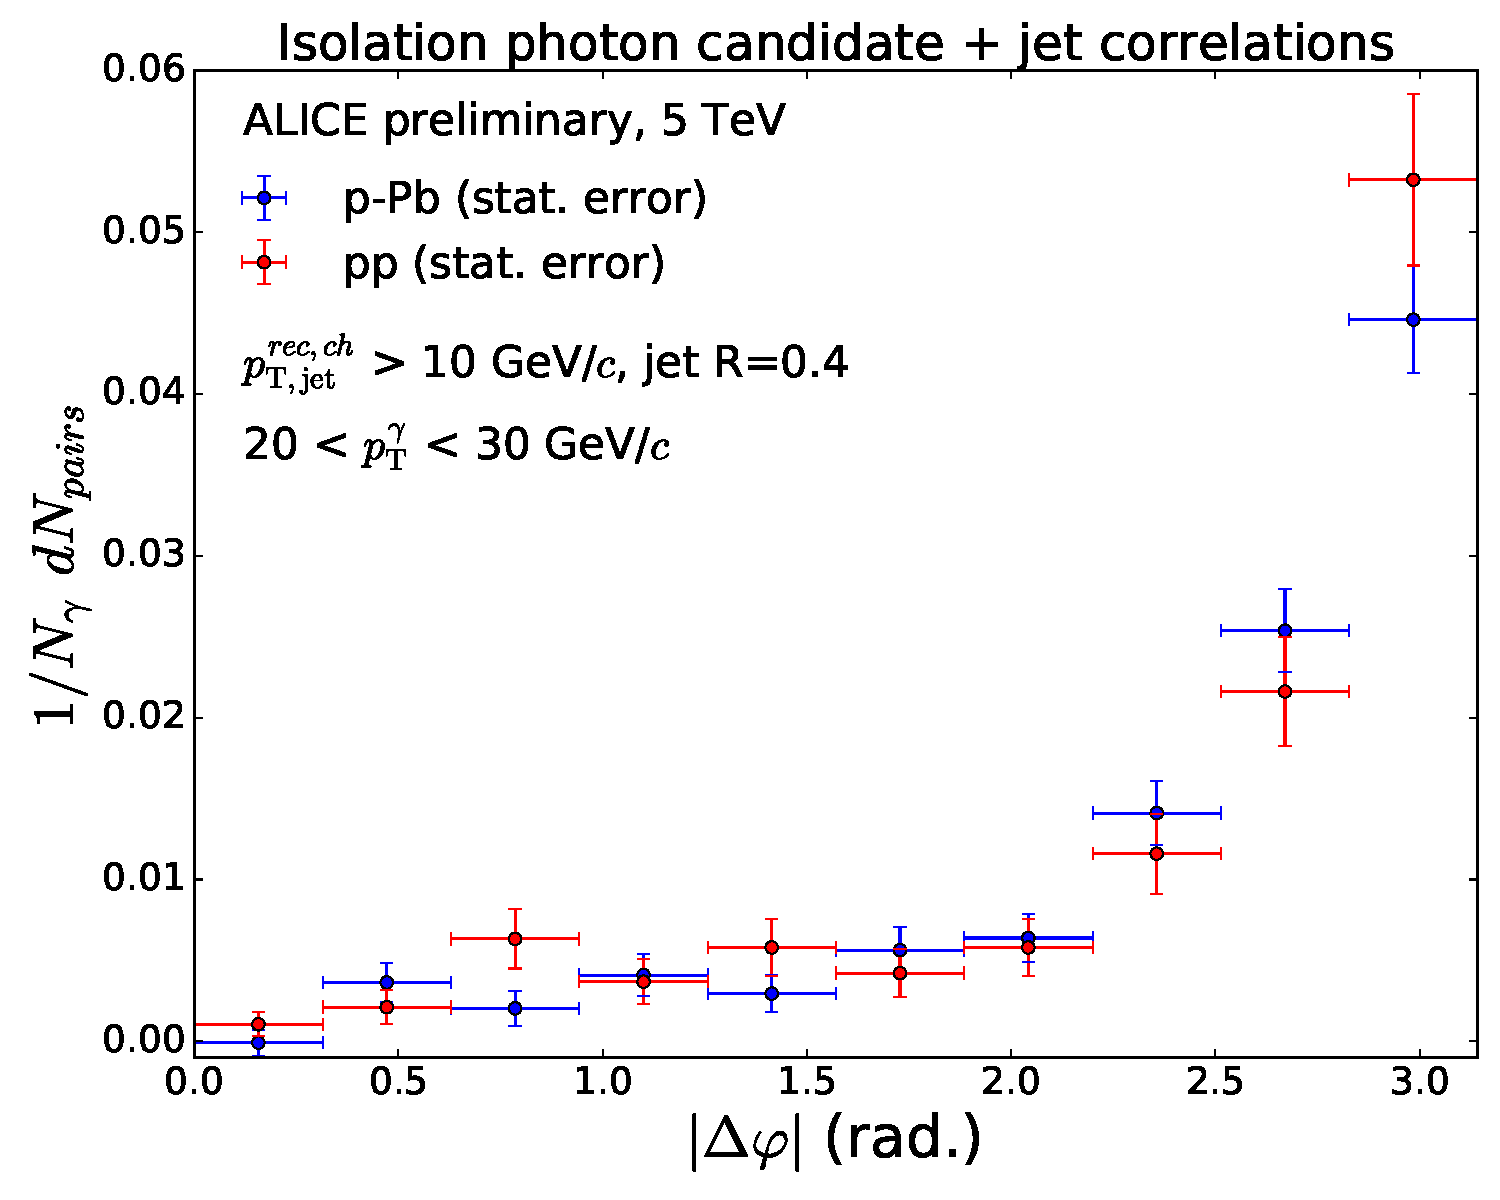
\includegraphics[width=0.7\textwidth]{GammaJet/Isolation_photon_candidate_jet_correlations.pdf}
\caption{$\Delta \phi$ distribution for photons with transverse momentum between 20 and 30 \GeVc recoiling against a jet with a reconstructed transverse greater than 10 \GeVc. The total number of trigger photons is used for normalization.}
\label{fig:isoGammaCandiJetCorr}
\end{figure}

\FloatBarrier
\subsection{DNN vs. $\lambda_0^2$ shower-shape cuts}
For most of our purposes, we use $\lambda_0^2$ as the variable we cut on to do the shower-shape cut. In this section, however, we compare correlations computed with the deep neural net (DNN) being used for the shower shape cut to the $\lambda_0^2$-cut correlations. Figure \ref{fig:DNNlambda} shows a comparison of DNN to $\lambda_0^2$ correlations for our two most important observables, $\Delta \phi$ and $x^{obs}_{Pb}$.

\begin{figure}
    \centering
    \includegraphics[width=0.24\textwidth]{GammaJet/pp_pPb_correlations/hadj_dPhipp_data_Comparison.pdf}
    \includegraphics[width=0.24\textwidth]{GammaJet/pp_pPb_correlations/hadj_dPhipPb_data_Comparison.pdf} \\
    \includegraphics[width=0.24\textwidth]{GammaJet/pp_pPb_correlations/hadj_XobsPbpp_data_Comparison.pdf}
    \includegraphics[width=0.24\textwidth]{GammaJet/pp_pPb_correlations/hadj_XobsPbpPb_data_Comparison.pdf}
    \caption{A comparison of $\gamma$-jet correlations computed using the deep neural net (DNN) for the shower shape cut to correlations computed using $\lambda_0^2$. Top row are $\Delta \phi$ correlations, bottom row is $x^{obs}_{Pb}$. The left comumn contains pp correlations and the right column contains pPb correlations.}
    \label{fig:DNNlambda}
\end{figure}

As seen in Figure \ref{fig:DNNlambda}, the DNN and $\lambda_0^2$ correlations are generally within uncertainty of each other. However, we do see some differences in shape between the correlations generated using the DNN cut and the ones generated using the $\lambda_0^2$ cut.

\FloatBarrier
\subsection{Comparison to pp and pPb Monte-Carlo}
In this section, we compare our data to simulations, in order to test the theory employed in our modeling of the data. Specifically, the 13def pPb and 17q pp data from ALICE are compared to to the 17g6a1 pPb $\gamma$-jet Monte-Carlo simulation data (which uses Pythia and DPMJET) and the 18b10a pp $\gamma$-jet Monte-Carlo simulation data (which uses Pythia), respectively. In order to do the comparison, we create $\gamma$-jet correlations using the same steps outlined in Section \ref{sec:GammaJetProcedure} for the 13def and 17q data, with two differences. A correction is made for the boosting of $\eta$ in the center-of-mass for the 17g6a1 results, which is the same as the one used for the 13d and 13e samples, as described in Section \ref{sec:GammaJetProcedure}.

The first of these differences is that the shower-shape background subtraction using Equation \ref{eq:FinalSubtraction} is not done. This is because the Monte-Carlo simulations are used to obtain the purities used in the subtraction in Equation \ref{eq:FinalSubtraction}, and Monte-Carlo simulations are exactly what is being evaluated in this section. The second of these differences is tied into the format that simulation data comes in. The simulation data is divided into $p_T$ "hats", which are data sets that each contain data in a specific interval of hard-scattering $p_T$. When the $p_T$ hats are added together, they must be weighted. The hard-scattering $p_T$ values and the weights for each $p_T$ hat used in our analysis for the 17g6a1 simulation can be seen in Table X. The 18b10a data has a built-in weighting system for the $p_T$ hats used, so we do not need to worry about that for 18b10a.

\begin{table}
    \centering
    \begin{tabular}{c|c c}
        $p_T$ hat & $p_T^{hard}$ range & weight \\
        \hline
        1 & 5-11 & $1.60*10^{-11}$ \\
        2 & 11-21 & $2.72*10^{-12}$ \\
        3 & 21-36 & $3.69*10^{-13}$ \\
        4 & 36-57 & $6.14*10^{-14}$ \\
        5 & 57-84 & $1.27*10^{-14}$
    \end{tabular}
    \caption{A table of the 17g6a1 $p_T$ hats used in this analysis, which includes the hard-scattering $p_T$ and weight of each $p_T$ hat}
    \label{tab:pthats}
\end{table}

Figure \ref{fig:data_simulation_correlation} shows a comparison of $\gamma$-jet correlations from the 13def pPb data with those from the 17g6a1 Monte-Carlo simulation results and of correlations from the 17q pp data with those from the 18b10a simulation results. The observables used are $\Delta \phi$ and $x^{obs}_{Pb}$. As seen in Figure \ref{fig:data_simulation_correlation}, the simulated correlations bear a resemblance to the general shape of the simulations from the data, but they do not capture many, if any at all, of the more complex behavior, such as of bumps or fluctuations outside of a very simplified model. This is somewhat less true of pp data than it is for pPb. However, the most extreme difference between data and simulation is the one in the $x^{obs}_{Pb}$ correlation in pPb: the data shows a slight peak at $x^{obs}_{Pb}$ $\approx$ 0.01, and a smoother curve down to the right than the curve up from the left of the peak, but generally a flat shape; the Monte-Carlo, on the other hand, shows a much sharper peak at $x^{obs}_{Pb}$ $\approx$ 0.018, and barely any counts below the peak.

\begin{figure}
    \centering
    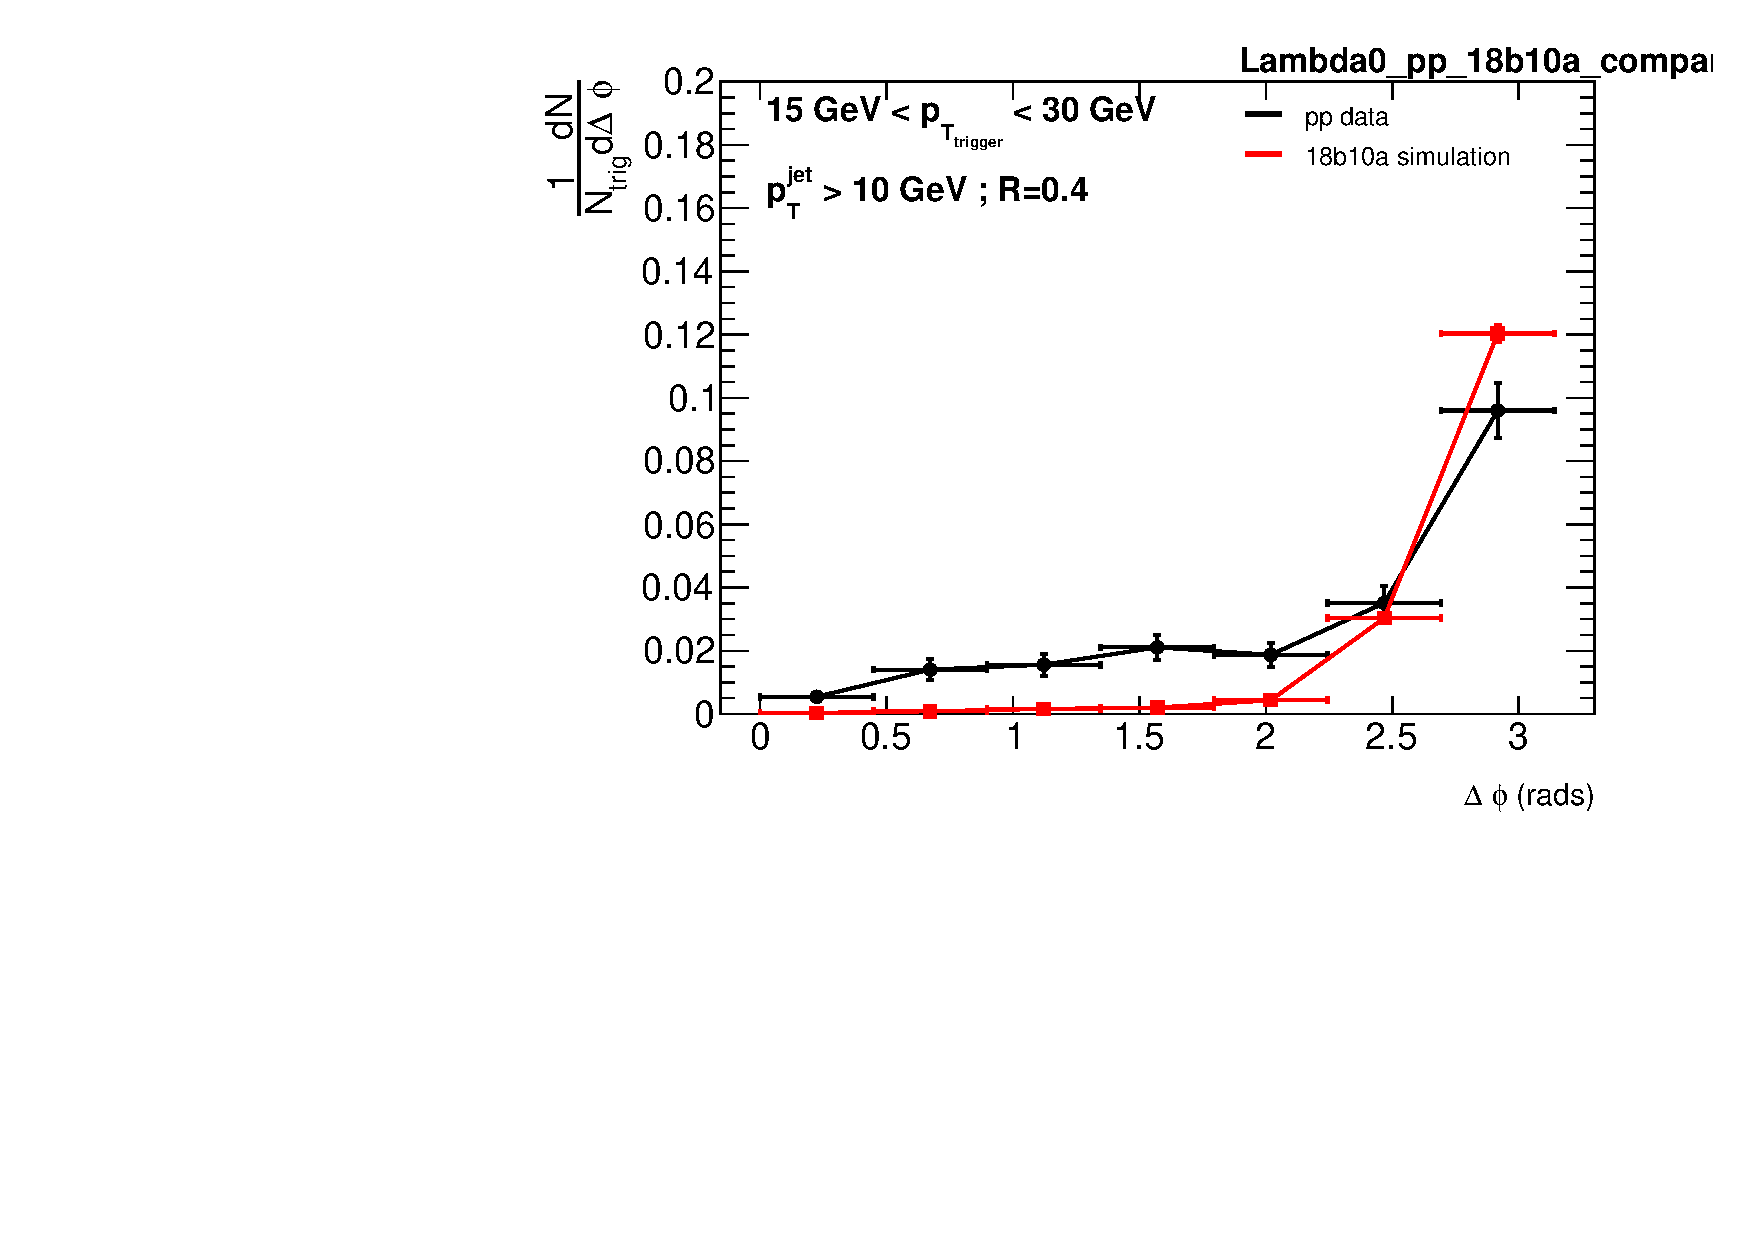
\includegraphics[width=0.49\textwidth]{GammaJet/pp_pPb_correlations/sig_dPhiLambda0_pp_18b10a_comparison_Comparison.pdf}
    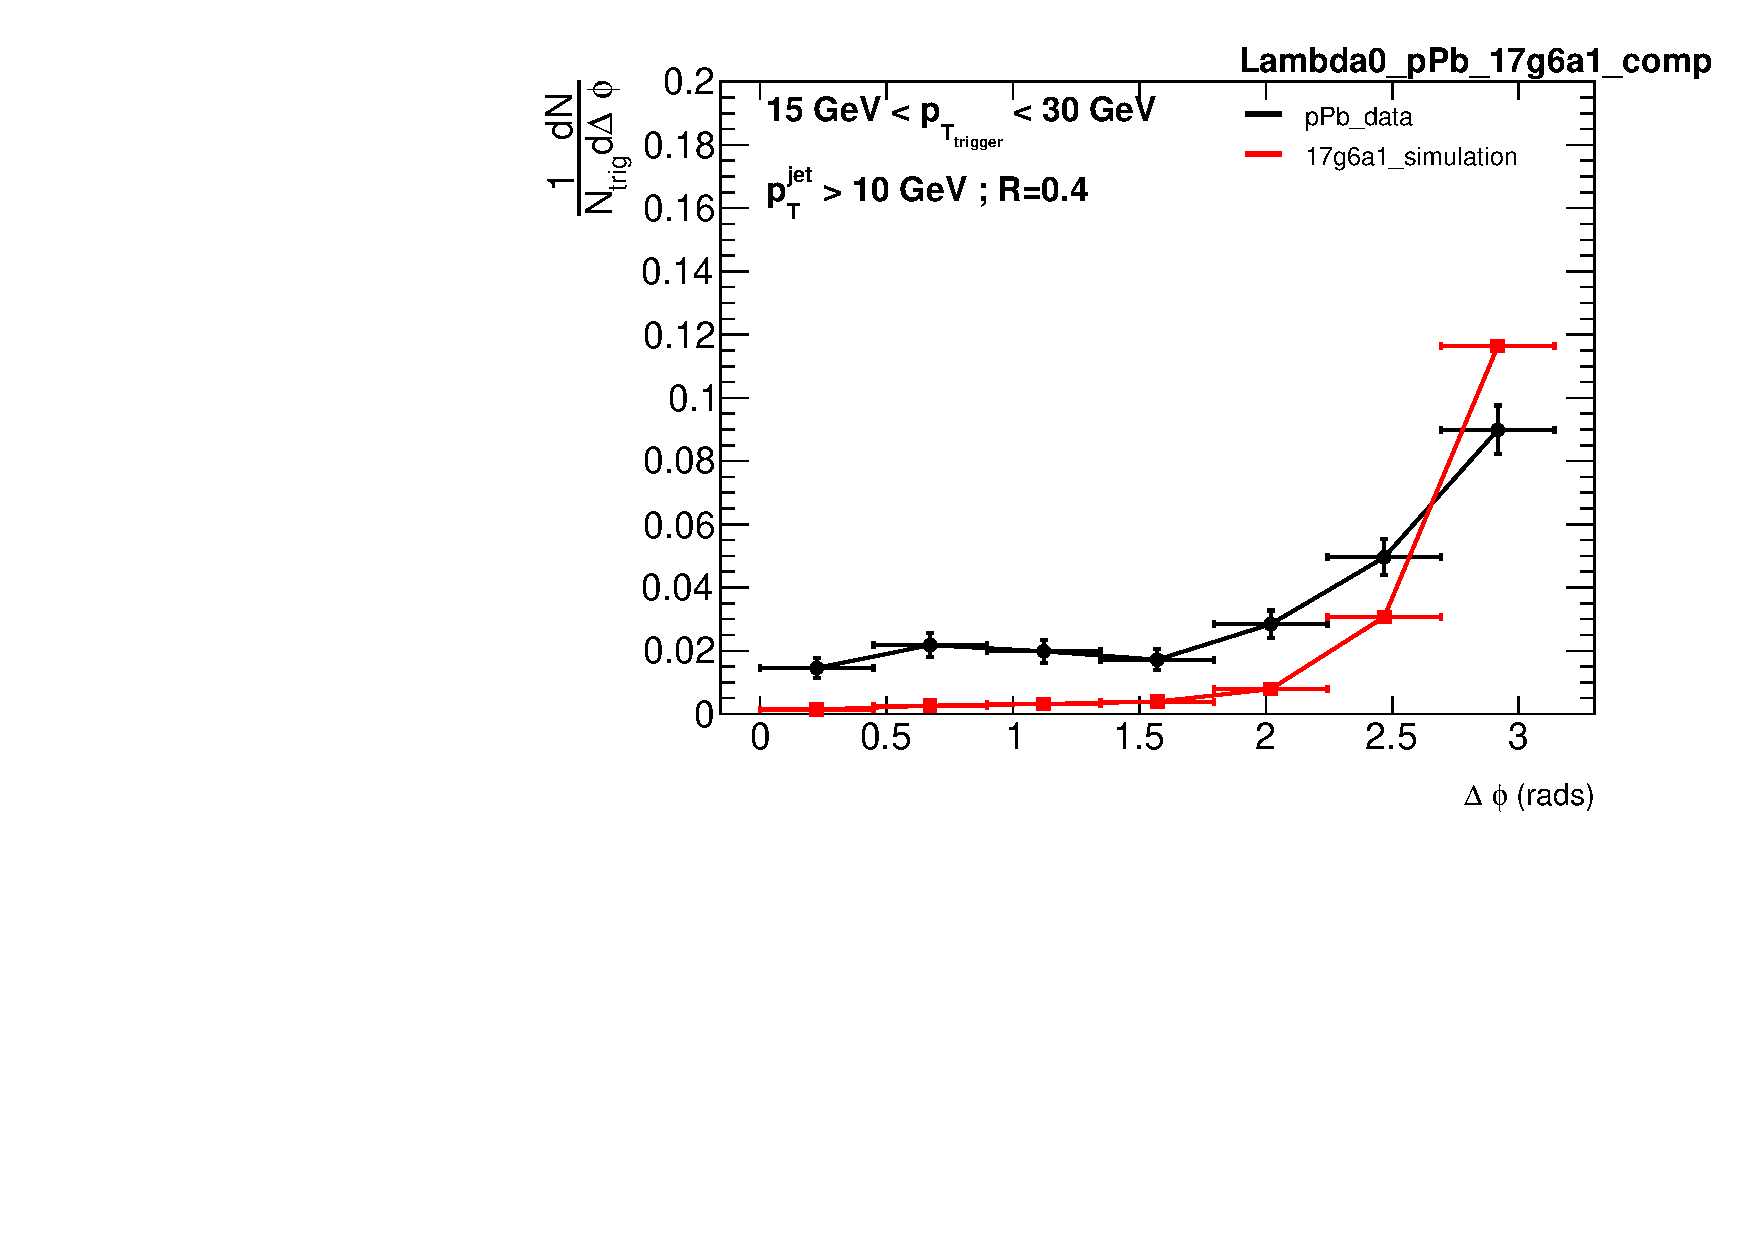
\includegraphics[width=0.49\textwidth]{GammaJet/pp_pPb_correlations/sig_dPhiLambda0_pPb_17g6a1_comparison_Comparison.pdf} \\
    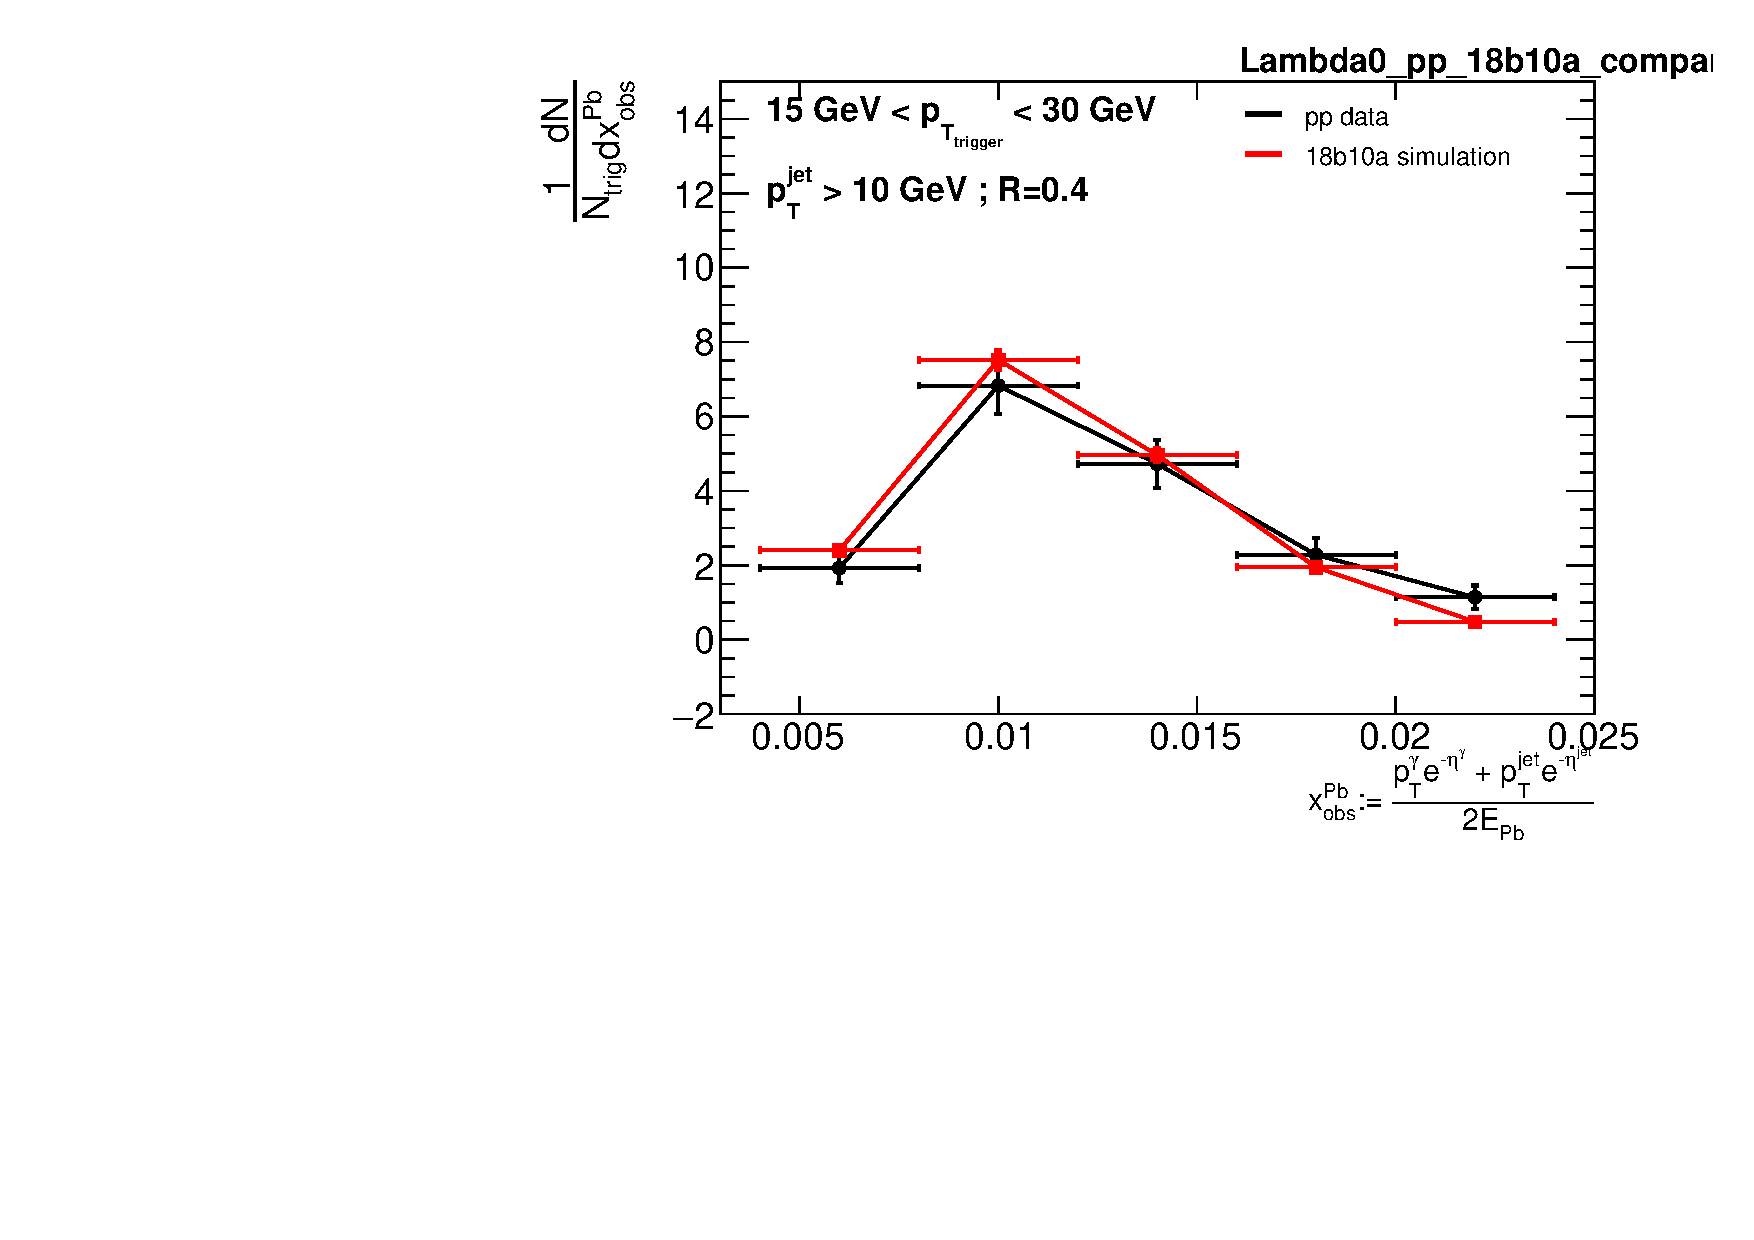
\includegraphics[width=0.49\textwidth]{GammaJet/pp_pPb_correlations/sig_XobsPbLambda0_pp_18b10a_comparison_Comparison.pdf}
    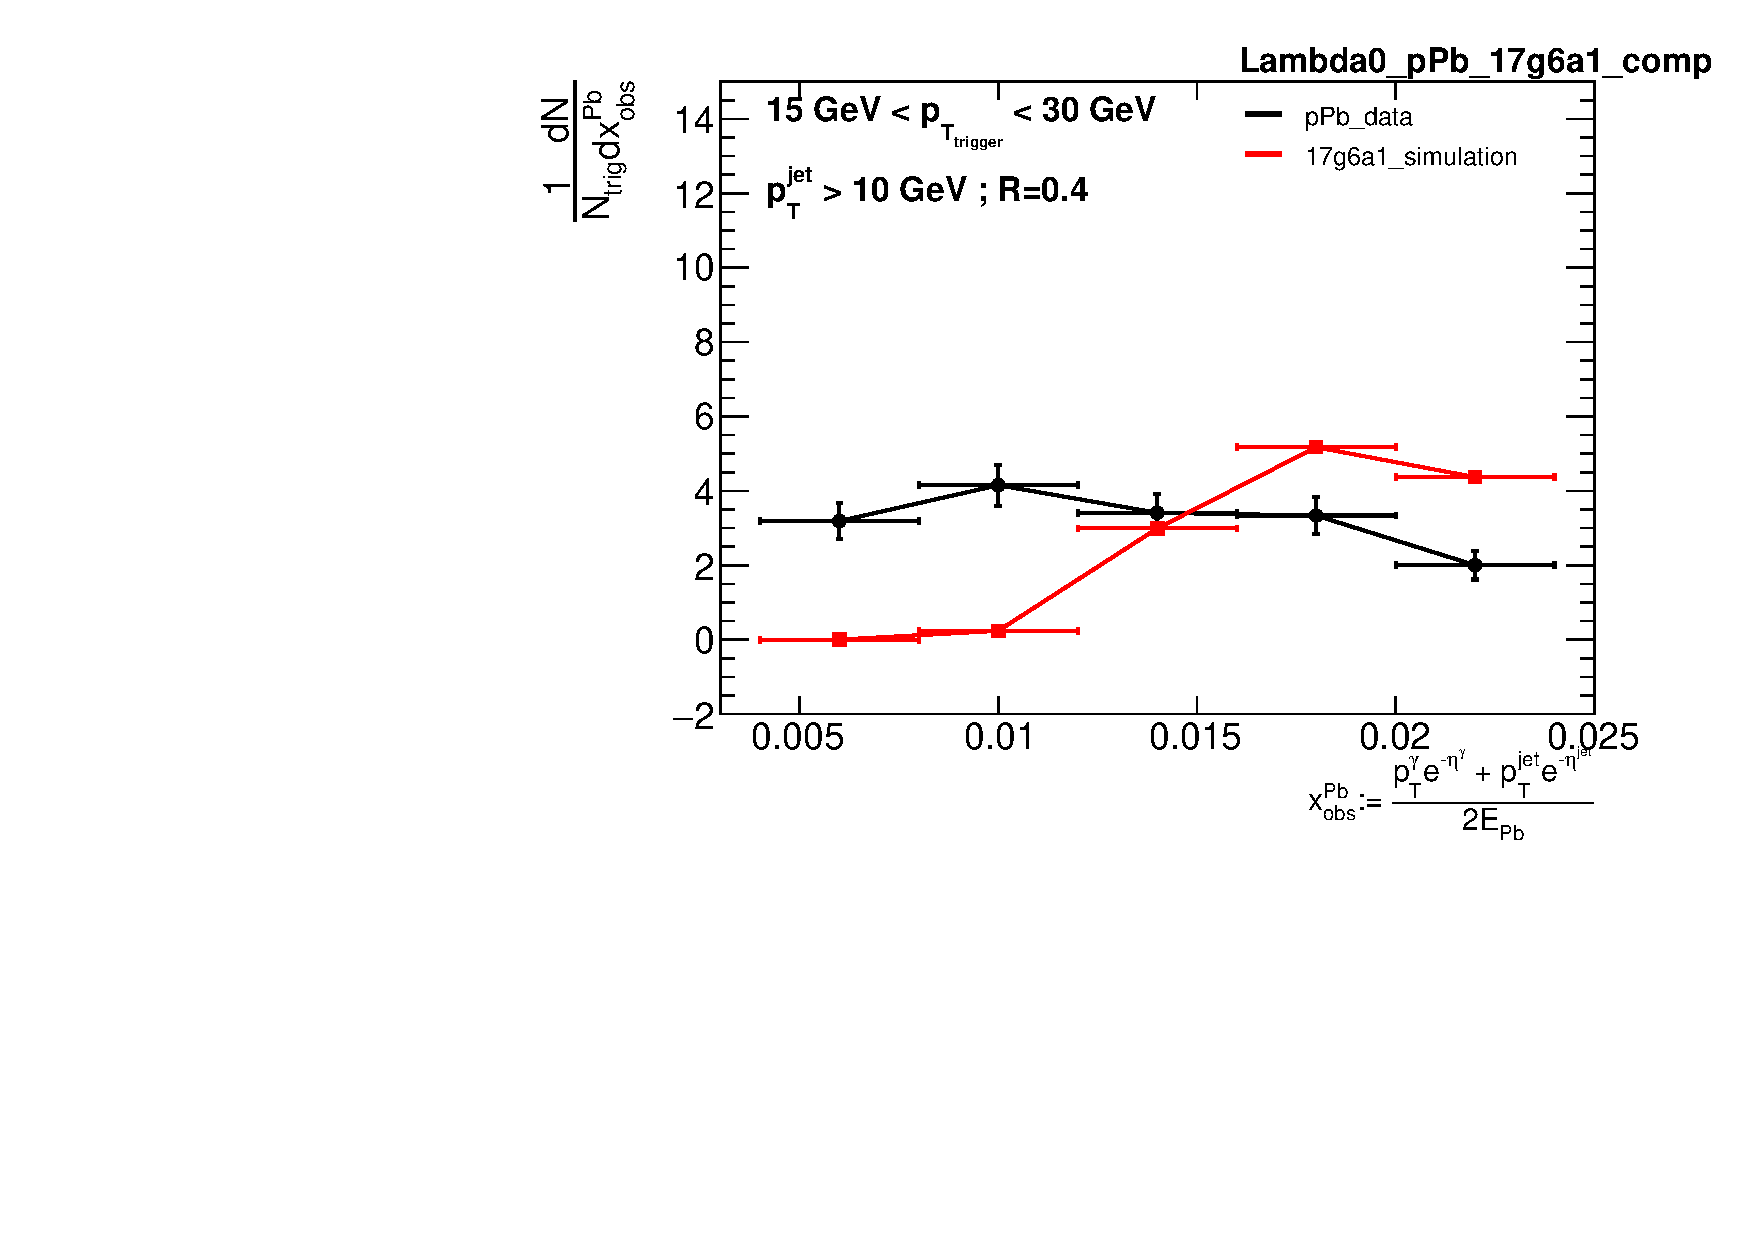
\includegraphics[width=0.49\textwidth]{GammaJet/pp_pPb_correlations/sig_XobsPbLambda0_pPb_17g6a1_comparison_Comparison.pdf}
    \caption{A comparison of $\gamma$-jet correlations computed using Monte-Carlo simulations to correlations computed using $\lambda_0^2$. Top row are $\Delta \phi$ correlations, bottom row is $x^{obs}_{Pb}$. The left comumn is a comparison of 17q pp data correlations with 18b10a pp Monte-Carlo correlations, and the right column is a comparison of 13def pPb data correlations with 17g6a1 pPb Monte-Carlo correlations.}
    \label{fig:data_simulation_correlation}
\end{figure}


\FloatBarrier
\subsection{Reconstructed-level results}
In this section, we present the reconstructed-level results, which will be corrected by detector smearing effects in Section~\ref{sec:unfolding}. The $p_T$ range is 20-30 \GeVc. Accordingly, the the shower-shape background subtraction in Equation \ref{eq:FinalSubtraction} is not done.

Figure~\ref{fig:ResultRecoLevel_jetpt} shows a comparison between the $\gammaiso$--jet correlations and \textsc{Pythia} photon+jet simulation. The simulation is not normalized to the data, but rather it is normalized by the number of trigger photons used. Good agreement is observed between the data and the simulation, both in shape and magnitude. 

\begin{figure}[h]
\centering
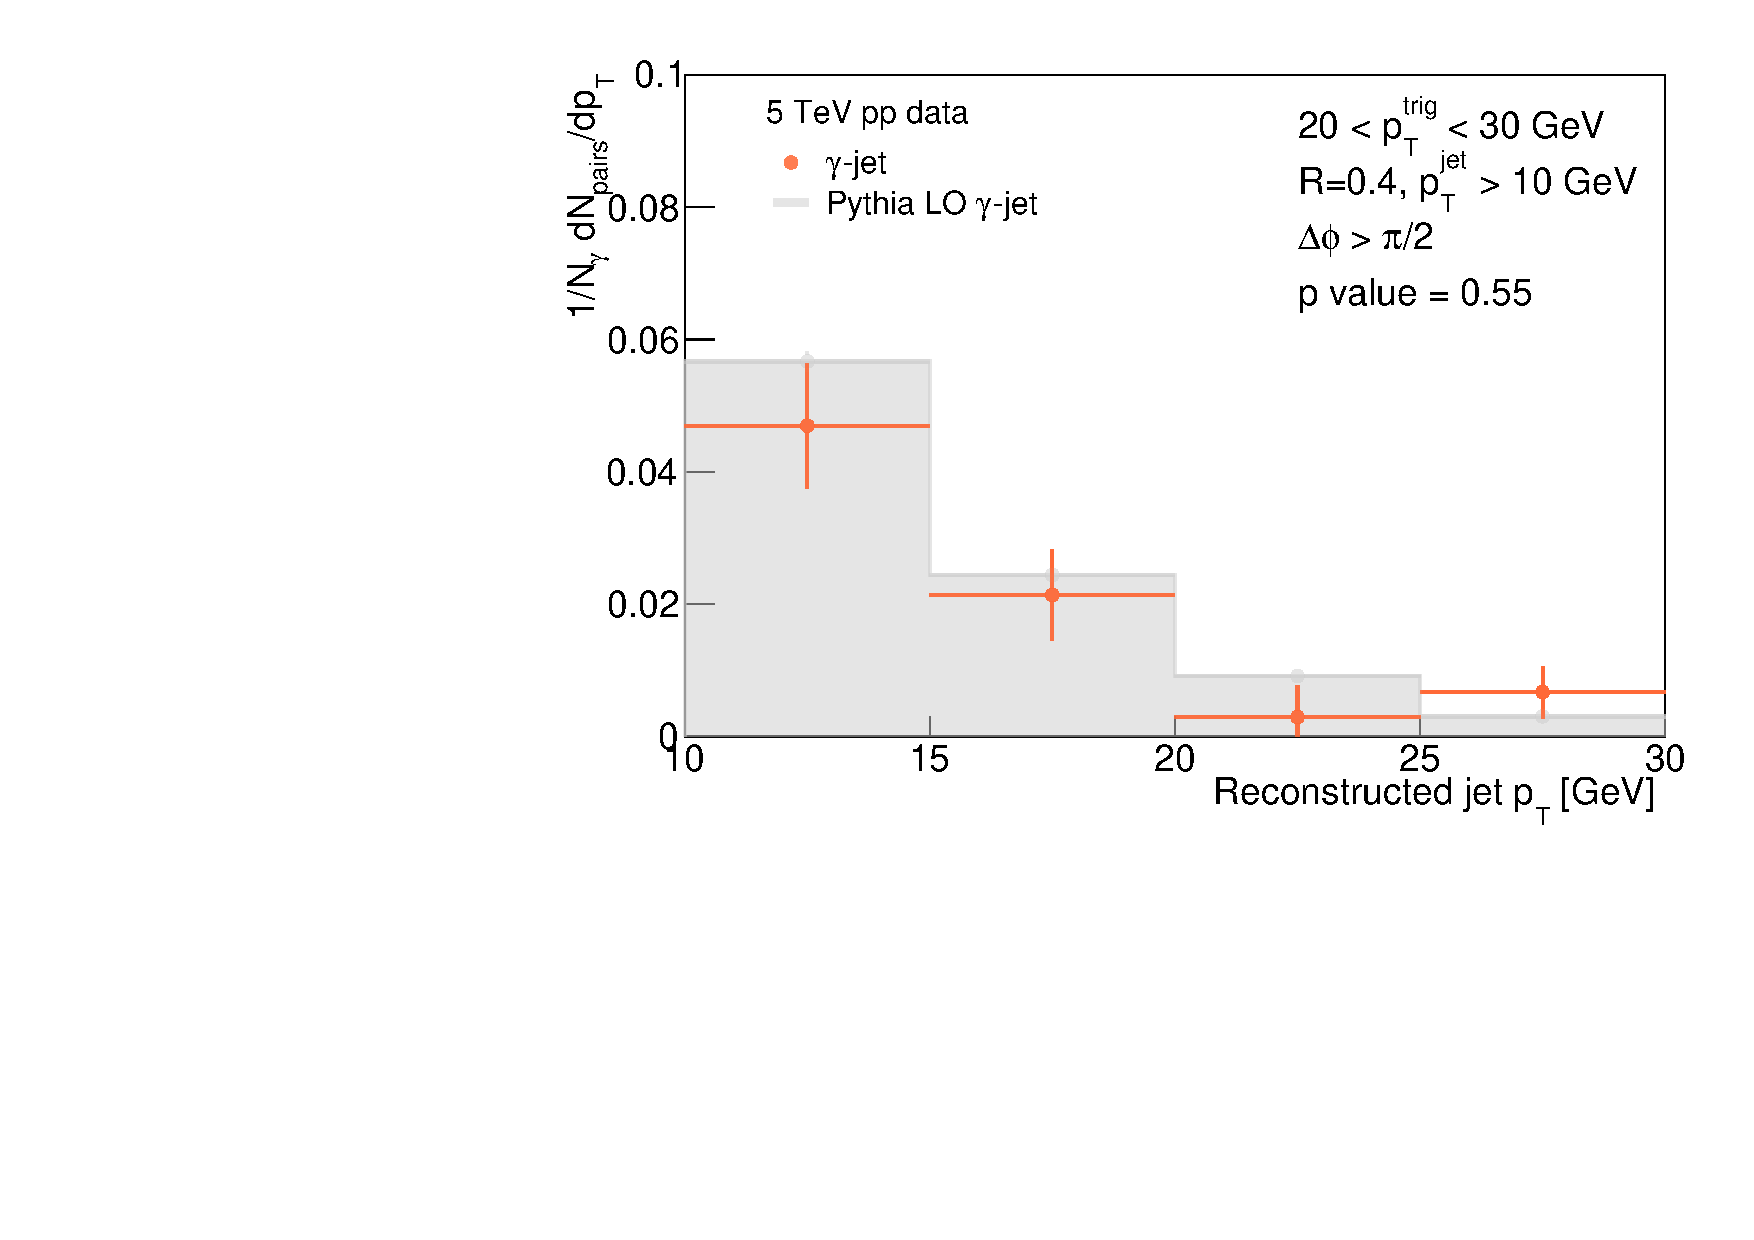
\includegraphics[width=0.495\textwidth]{GammaJet/Final_jetpt_step1_purity0_500_DATANAME_Out_Skimmed_17q_clus20_0_max30_0_JET_R0_4_PT_10_0_Iso1_5_root_WithMC}
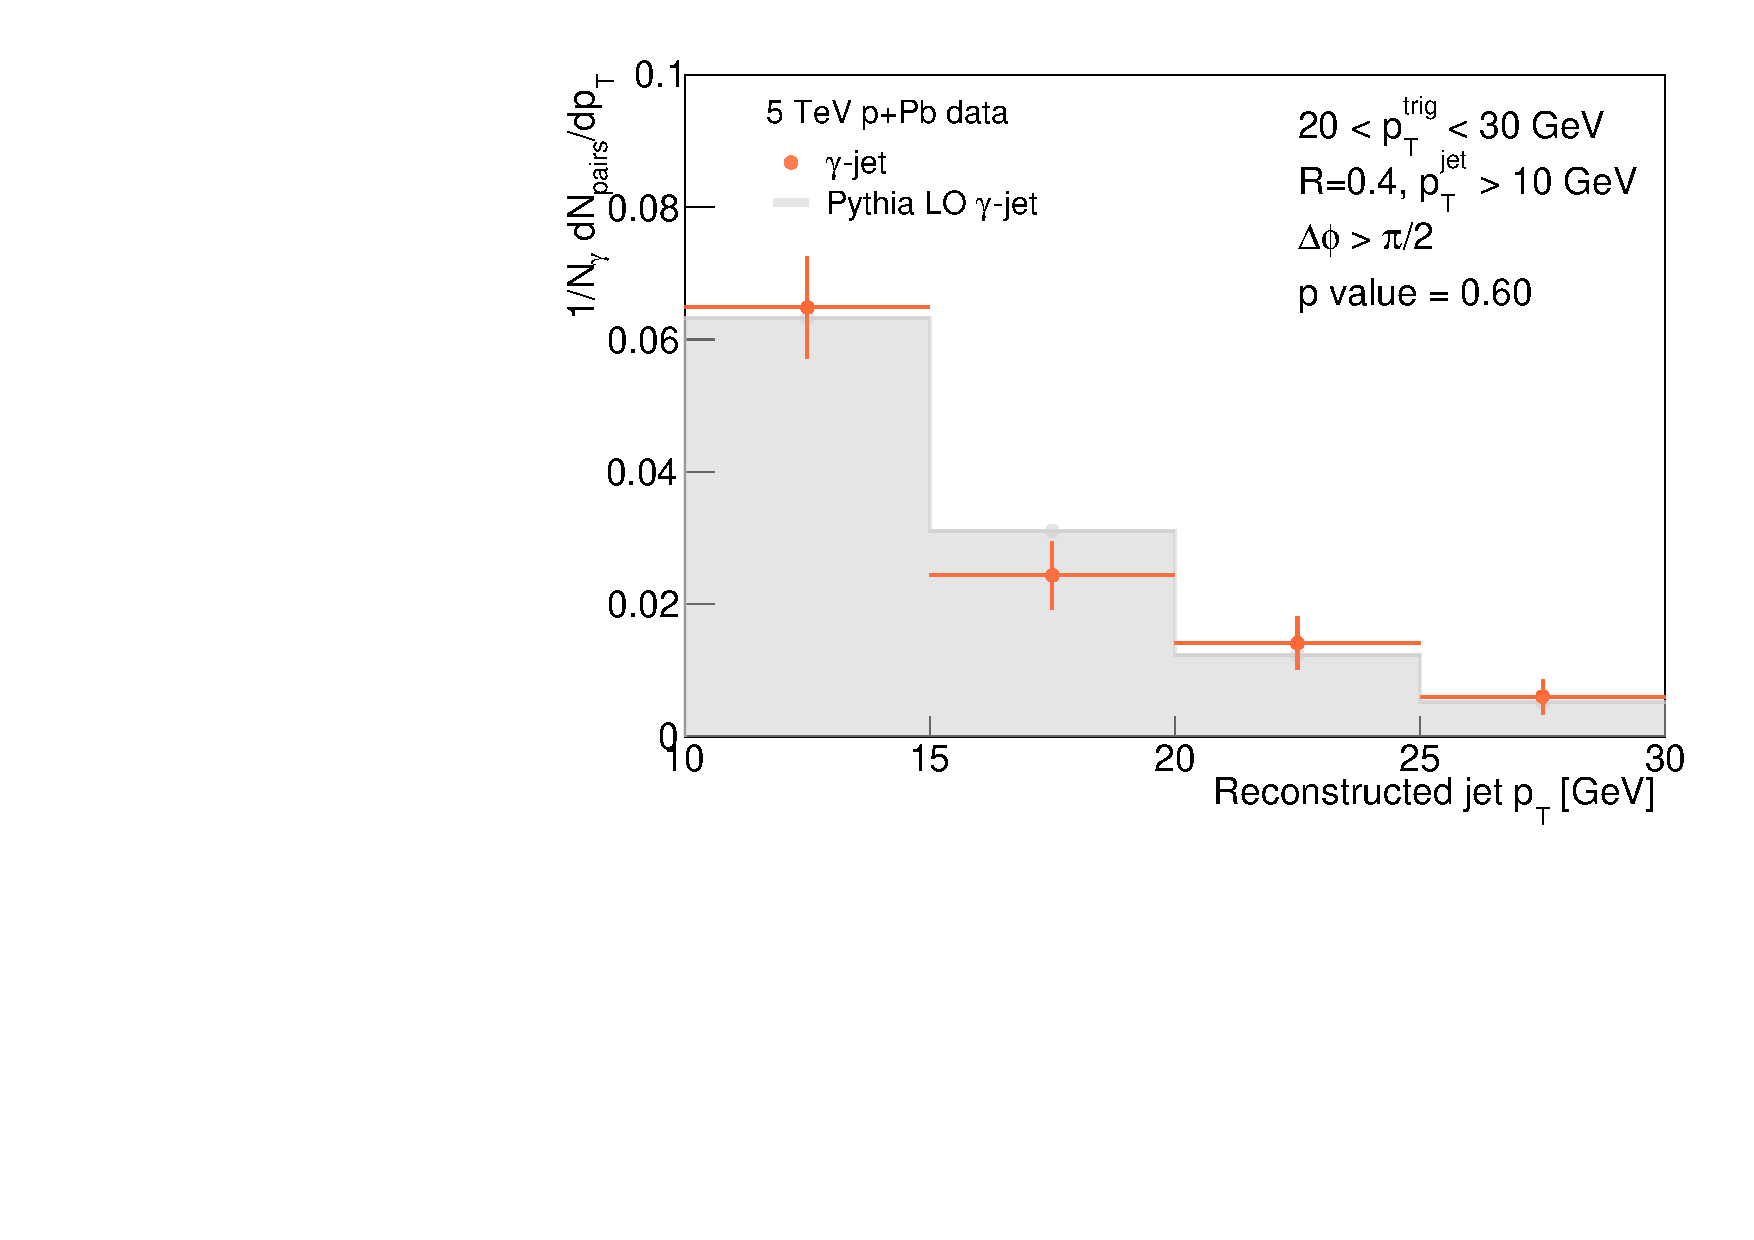
\includegraphics[width=0.495\textwidth]{GammaJet/Final_jetpt_step1_purity0_500_DATANAME_Out_Skimmed_13def_clus20_0_max30_0_JET_R0_4_PT_10_0_Iso1_5_root_WithMC}\\
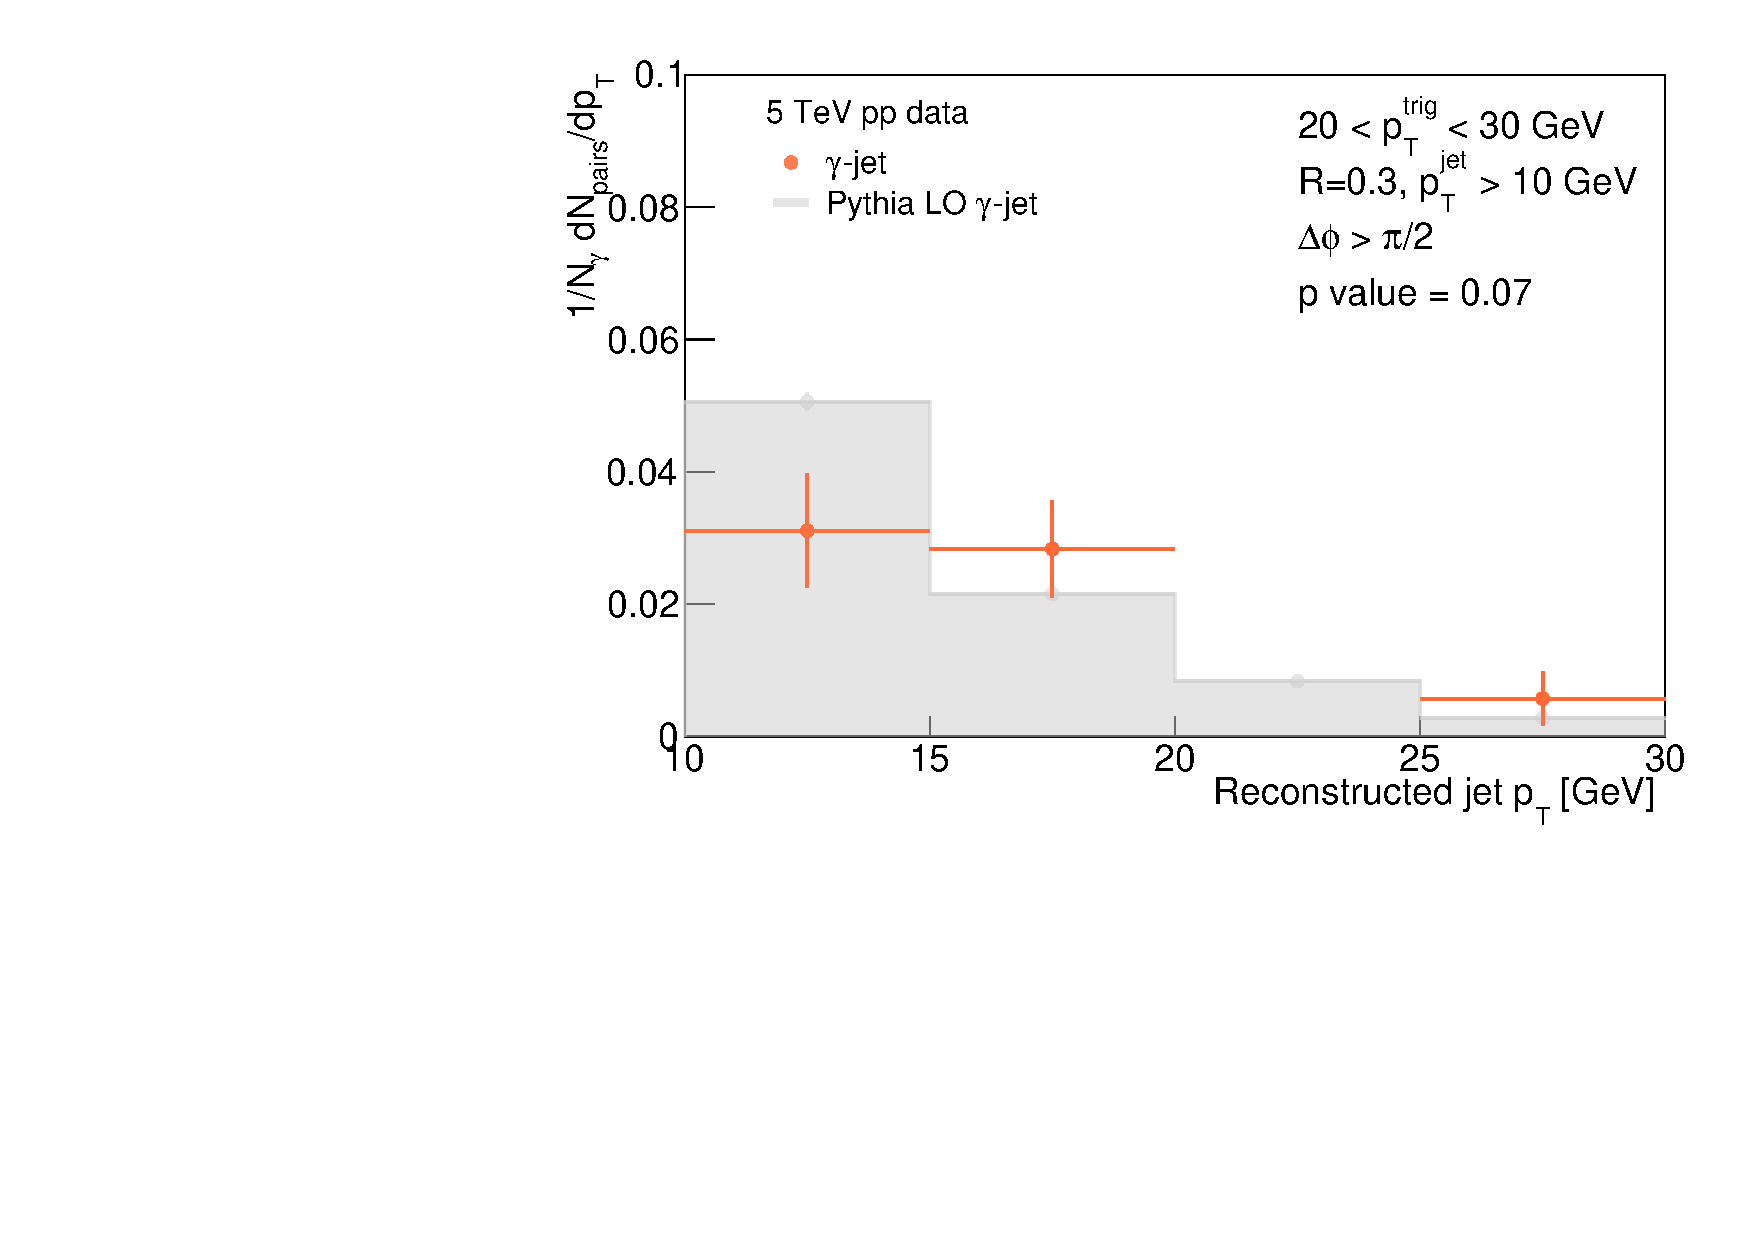
\includegraphics[width=0.495\textwidth]
{GammaJet/Final_jetpt_step1_purity0_500_DATANAME_Out_Skimmed_17q_clus20_0_max30_0_JET_R0_3_PT_10_0_Iso1_5_root_WithMC}
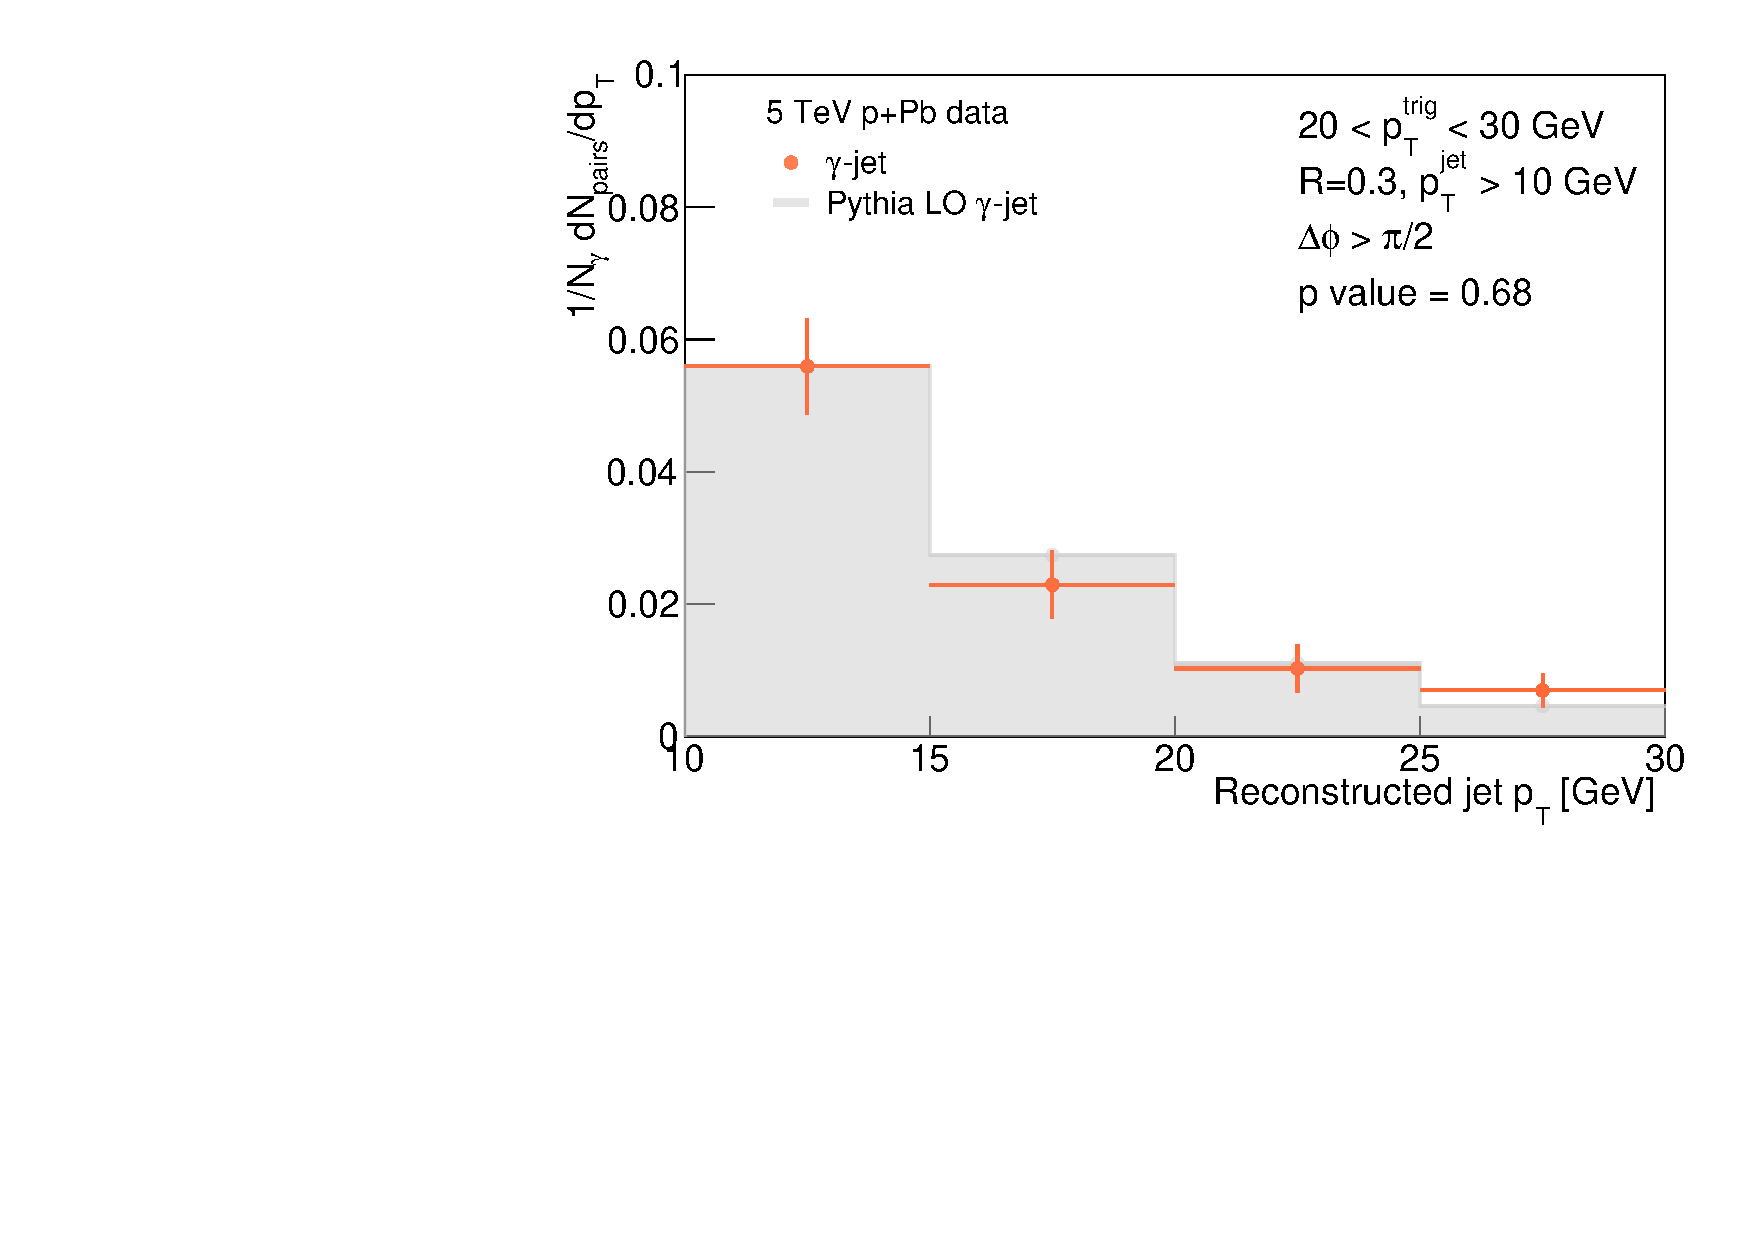
\includegraphics[width=0.495\textwidth]{GammaJet/Final_jetpt_step1_purity0_500_DATANAME_Out_Skimmed_13def_clus20_0_max30_0_JET_R0_3_PT_10_0_Iso1_5_root_WithMC}
\caption{Transverse momentum spectrum for jets recoiling against an $\gammaiso$ photon with 20--30 \GeVc. The distributions are normalized by the total number of trigger photons. The error bars represent statistical uncertainty only.}
\label{fig:ResultRecoLevel_jetpt}
\end{figure}


\begin{figure}[h]
\centering
\includegraphics[width=0.495\textwidth]{GammaJet/FinalResult_jetptR0_3}
\includegraphics[width=0.495\textwidth]{GammaJet/FinalResult_jetptR0_4}\\
\includegraphics[width=0.495\textwidth]{GammaJet/FinalResult_Pionjetpt_R0_3}
\includegraphics[width=0.495\textwidth]{GammaJet/FinalResult_Pionjetpt_R0_4}\\
\includegraphics[width=0.495\textwidth]{GammaJet/FinalResult_IsoPionjetpt_R0_3}
\includegraphics[width=0.495\textwidth]{GammaJet/FinalResult_IsoPionjetpt_R0_4}\\
\caption{Transverse momentum spectrum for jets recoiling against an $\gammaiso$ photon (upper row), $\pi^{0}$ (middle row), and isolated $\pi^{0}$ with 20--30 \GeVc. The distributions are normalized by the total number of triggers. The error bars represent statistical uncertainty only.}
\label{fig:FinalResults_RecoLevel}
\end{figure}

\begin{figure}[h]
\centering
\includegraphics[width=0.495\textwidth]{GammaJet/Final_jetpt_step1_purity0_500_DATANAME_Out_Skimmed_13def_clus20_0_max30_0_JET_R0_3_PT_10_0_Iso1_5_root}
\includegraphics[width=0.495\textwidth]{GammaJet/Final_jetpt_step1_purity0_500_DATANAME_Out_Skimmed_13def_Lambda_clus20_0_max30_0_JET_R0_4_PT_10_0_Iso1_5_root}\\
\includegraphics[width=0.495\textwidth]{GammaJet/Final_jetpt_step1_purity0_500_DATANAME_Out_Skimmed_17q_clus20_0_max30_0_JET_R0_3_PT_10_0_Iso1_5_root}
\includegraphics[width=0.495\textwidth]{GammaJet/Final_jetpt_step1_purity0_500_DATANAME_Out_Skimmed_17q_Lambda_clus20_0_max30_0_JET_R0_4_PT_10_0_Iso1_5_root}
\caption{Transverse momentum spectrum for jets recoiling against an $\gammaiso$ photon, $\pi^{0}$, and isolated $\pi^{0}$ with 20--30 \GeVc. The distributions are normalized by the total number of triggers. The error bars represent statistical uncertainty only.}
\label{fig:FinalResults_ComparisonGammaPion}
\end{figure}

%%%%%%%%%%%%%%%%%%%%%%%%%%%%%%%%%%%%%%%%%%%%%%%%%%%%%%%%%%%%%%%%%%%%%%%%%%%%%%%%%%%%%%%%%%%%%%%%%%%%%%%%%%%%%%%%%%%%%%%%%%%%%%%%%%%%%%%%%%%%%%%%%%%%%%%%%%%%%%%%%%%%%%%%%%%%%%%%%%%%%%%%%%%%%%%%%%%%%%%%%%%%%%%%%%%%%%%%%%%%%%%%%%%%%%%%%%%%%%%%%%%%%%%%%%%%%%%%%%%%%%%%%%%%%%%%%%%%%%%%%%%%%%%%%%%%%%%%%%%%%%%%%%%%%%%%%%%%%%%%%%%%%%%%%%%%%%%%%%%%%%%%%%%%%%%%%%%%%%%%%%%%%%%%%%%%%%%%%%%%%%%%%%%%%%

%%[Commenting out sections on Xobs, not for preliminary results. Miguel, September 17th.]
%\subsection{Observable fractional momentum, \xobs}
%Following Ref.~\cite{Klasen:2017dsy}, we construct the following observable: 
%\begin{equation}
%\xobs = \frac{\left(\pt^{\gamma}e^{-\eta^{\gamma}} + \pt^{\mathrm{jet}}e^{-\eta^{\mathrm{jet}}}\right)}{2E_{\mathrm{pPb}}}. 
%\end{equation}

%This variable is sensitive to Bjorken $x$ in nuclei, and is similar to variables used by the H1 and ZEUS experiments at the HERA electron-proton collider for determination of proton and photon PDFs~\cite{Klasen:2002xb,Adloff:2000bs}. 

%We will compare our results with next-to-leading order calculations matched with parton showers (Pythia + POWHEG)~\cite{Klasen:2017dsy} made for the kinematic range used in this analysis. These calculations with commonly used nuclear PDFs predict differences in p-Pb and pp data of the order of 10--20$\%$ in this variable, due to its sensitivity to Bjorken $x$ in the gluon shadowing region in nuclei. The difference between the results obtained using different sets of nPDFs also disagree by 10--20$\%$, with an uncertainty of the order of X$\%$. More detailed description of the sensitivity of this \xobs variable on Bjorken-x in nuclei is shown in Appendix [yet to be filled]. 

%\subsubsection{Correlations tagged with $\gammaiso$ candidates and $\ydecay$}
%Figure~\ref{fig:Xobs_inSRandBR} show the \xobs~distribution measured in pp and p-Pb %data, for signal and background regions.
%This distribution peaks around $\xobs\approx0.003$ in all cases and for the most part the measurements using the different shower-shape variables are compatible. There are hints of difference between the signal region ($\gammaiso$ candidates) and the background region ($\ydecay$). This is investigated further in the following sections. 

%\begin{figure}[h]
%\center
%\includegraphics[width=0.49\textwidth]{GammaJet/hSR_XobsPbpp_data_Comparison.pdf}
%\includegraphics[width=0.49\textwidth]{GammaJet/hSR_XobsPbpPb_data_Comparison.pdf}\\
%\includegraphics[width=0.49\textwidth]{GammaJet/hBR_XobsPbpp_data_Comparison.pdf}
%\includegraphics[width=0.49\textwidth]{GammaJet/hBR_XobsPbpPb_data_Comparison.pdf}
%\caption{\xobs~distribution for pp (left) and p-Pb data (right). The upper row shows the distributions for $\gammaiso$ candidates (signal region) and the bottom row for $\ydecay$ candidates. The error bar represents statistical uncertainty only.}
%\label{fig:Xobs_inSRandBR}
%\end{figure}

%\FloatBarrier
%\subsubsection{Correlations tagged with $\gammaiso$}
%Figure~\ref{fig:Xobs_FinalSubtraction} shows the distributions for $\xobs$ correlations, obtained using the measured purity and Equation~\ref{eq:FinalSubtraction}. The resulting distributions are, for the most part, compatible within uncertainty among the different shower-shape variables. The largest statistical variation in the the $\emax$ case comes from the lower-efficiency of this variable at selecting single photons. 

%\begin{figure}[h]
%\center
%\includegraphics[width=0.49\textwidth]{GammaJet/hadj_XobsPbpp_data_Comparison.pdf}
%\includegraphics[width=0.49\textwidth]{GammaJet/hadj_XobsPbpPb_data_Comparison.pdf}
%\caption{$X_{\mathrm{obs}}^{\mathrm{Pb}}$ for pp (left) and p-Pb data (right). The $\ydecay$ contribution is subtracted following Equation \ref{eq:FinalSubtraction}. The error bar represents the combination of statistical uncertainty in the data and the statistical uncertainty in the purity measurement. }
%\label{fig:Xobs_FinalSubtraction}
%\end{figure}

%\FloatBarrier
%\subsubsection{Distributions from photon+jet simulation}

%Figure~\ref{fig:Xobs_MC} shows the \xobs from photon+jet simulation.  
%\begin{figure}[h]
%\center
%\includegraphics[width=0.49\textwidth]{GammaJet/hSR_XobsPb17g6a1_data_Comparison.pdf}
%\includegraphics[width=0.49\textwidth]{GammaJet/hSR_XobsPb17g6a1_truths_Comparison.pdf}\\
%\caption{$\xobs$ distribution for photon+jet simulation. The left panels shows the distribution at the particle level (left) and the right panel shows it at the truth level (right). The error bar represents statistical uncertainty only.}
%\label{fig:Xobs_MC}
%\end{figure}


%\FloatBarrier
%\subsection{Jet dispersion, $\pTD$ }
%In this and the following section, we measure variables that are commonly used for used quark/gluon discriminators in HEP analyses~\cite{CMS-DP-2016-070,Aad:2016oit,Larkoski:2014pca}. These variables have also been used to study the modification of the fragmentation pattern of inclusive jets or jets selected for quark-like properties in nuclear collisions 
%bvj due to the formation of the quark-gluon plasma
%~\cite{Acharya:2018uvf}. 

%The jet $\pTD$ is defined as the second moment of the constituent $\pt$~distribution in the jet:
%\begin{equation}
%\pTD = \frac{\sqrt{\sum_{\mathrm{i track in jet}} i (\pt^{i})^{2}}}{ \sum_{\mathrm{i track in jet}} \pt^{i}}. 
%\end{equation}

%In the extreme case of few constituents carrying a large fraction of the jet momentum, $\pTD\to 1$, while in the case of large number of constituents $\pTD\to 0$.

%\subsubsection{Correlations tagged with $\gammaiso$ candidates and $\ydecay$}
%Figure~\ref{fig:PTD_inSRandBR} shows the \pTD~distributions measured in pp and p-Pb data, for signal and background regions.
%\begin{figure}%
%\center
%\includegraphics[width=0.49\textwidth]{GammaJet/hSR_pTDpPb_data_Comparison.pdf}
%\includegraphics[width=0.49\textwidth]{GammaJet/hSR_pTDpp_data_Comparison.pdf}\\
%\includegraphics[width=0.49\textwidth]{GammaJet/hBR_pTDpPb_data_Comparison.pdf}
%\includegraphics[width=0.49\textwidth]{GammaJet/hBR_pTDpp_data_Comparison.pdf}
%\caption{Jet dispersion for pp (left) and p-Pb data (right). The upper row shows the distributions for $\gammaiso$ candidates (signal region) and the bottom row for $\ydecay$ candidates. The error bar represents statistical uncertainty only.}
%\label{fig:PTD_inSRandBR}
%\end{figure}


%\FloatBarrier
%\subsubsection{Correlations tagged with $\gammaiso$}
%\begin{figure}[h]
%\center
%\includegraphics[width=0.49\textwidth]{GammaJet/hadj_pTDpp_data_Comparison.pdf}
%\includegraphics[width=0.49\textwidth]{GammaJet/hadj_pTDpPb_data_Comparison.pdf}
%\caption{Jet dispersion, \pTD, distribution for pp (left) and p-Pb data (right). The $\ydecay$ contribution is subtracted following Equation \ref{eq:FinalSubtraction}. The error bar represents the combination of statistical uncertainty in the data and the statistical uncertainty in the purity measurement.}
%\end{figure}

%\FloatBarrier
%\subsubsection{Distributions from photon+jet simulation}

%Figure~\ref{fig:Xobs_MC} shows the \pTD~from photon+jet simulation.  

%\begin{figure}[h]
%\center
%\includegraphics[width=0.49\textwidth]{GammaJet/hSR_pTD17g6a1_data_Comparison.pdf}
%\includegraphics[width=0.49\textwidth]{GammaJet/hSR_pTD17g6a1_truths_Comparison.pdf}\\
%\caption{Jet dispersion, $\pTD$, distribution for photon+jet simulation. The left panels shows the distribution at the particle level (left) and the right panel shows it at the truth level (right). The error bar represents statistical uncertainty only.}
%\label{fig:Xobs_MC}
%\end{figure}


%\FloatBarrier
%\subsection{Jet constituent multiplicity}
%Jet constituent  multiplicity scales with the color charge $(C_{F}/C_{A})$, so this quantity is a powerful discriminator for quark and gluon initiated jets~\cite{Aad:2016oit}. 

%\begin{figure}[h]
%\center
%\includegraphics[width=0.49\textwidth]{GammaJet/hSR_Multiplicitypp_data_Comparison.pdf}
%\includegraphics[width=0.49\textwidth]{GammaJet/hSR_MultiplicitypPb_data_Comparison.pdf}\\
%\includegraphics[width=0.49\textwidth]{GammaJet/hBR_Multiplicitypp_data_Comparison.pdf}
%\includegraphics[width=0.49\textwidth]{GammaJet/hBR_MultiplicitypPb_data_Comparison.pdf}
%\caption{Charged-particle multiplicity within jets for pp (left) and p-Pb data (right). The upper row shows the distributions for $\gammaiso$ candidates (signal region) and the bottom row for $\ydecay$ candidates. The error bar represents statistical uncertainty only.}
%\label{fig:JetMultiplicity_inSRandBR}
%\end{figure}

%\begin{figure}
%\center
%\includegraphics[width=0.49\textwidth]{GammaJet/hadj_Multiplicitypp_data_Comparison.pdf}
%\includegraphics[width=0.49\textwidth]{GammaJet/hadj_MultiplicitypPb_data_Comparison.pdf}
%\caption{Multiplicity distribution for pp (left) and p-Pb data (right), as calculated by Equation \ref{eq:FinalSubtraction}}
%\end{figure}

%\begin{figure}
%\center
%\includegraphics[width=0.49\textwidth]%{GammaJet/hSR_Multiplicity17g6a1_data_Comparison.pdf}
%\includegraphics[width=0.49\textwidth]{GammaJet/hSR_Multiplicity17g6a1_truths_Comparison.pdf}
%\caption{Multiplicity distribution for photon+jet simulation. The left panels shows the distribution at the particle level (left) and the right panel shows it at the truth level (right). The error bar represents statistical uncertainty only.}
%\end{figure}

%\FloatBarrier
%\subsection{$\frac{p_{T}^{jet}}{p_{T}^{trigger}}$ (Xj)}

%\begin{figure}
%\center
%\includegraphics[width=0.49\textwidth]{GammaJet/hSR_Xjpp_data_Comparison.pdf}
%\includegraphics[width=0.49\textwidth]{GammaJet/hSR_XjpPb_data_Comparison.pdf}\\
%\includegraphics[width=0.49\textwidth]{GammaJet/hBR_Xjpp_data_Comparison.pdf}
%\includegraphics[width=0.49\textwidth]{GammaJet/hBR_XjpPb_data_Comparison.pdf}
%\caption{Ratio of jet to photon momentum $x_{J}$ for pp (left) and p-Pb data (right). The upper row shows the distributions for $\gammaiso$ candidates (signal region) and the bottom row for $\ydecay$ candidates. The error bar represents statistical uncertainty only.}
%\end{figure}

%\begin{figure}
%\center
%\includegraphics[width=0.49\textwidth]{GammaJet/hadj_Xjpp_data_Comparison.pdf}
%\includegraphics[width=0.49\textwidth]{GammaJet/hadj_XjpPb_data_Comparison.pdf}
%\caption{Ratio of jet to photon momentum $x_{J}$ distribution for pp (left) and p-Pb data (right), as calculated by Equation \ref{eq:FinalSubtraction}}
%\end{figure}

%\begin{figure}
%\center
%\includegraphics[width=0.49\textwidth]{GammaJet/hSR_Xj17g6a1_data_Comparison.pdf}
%\includegraphics[width=0.49\textwidth]{GammaJet/hSR_Xj17g6a1_truths_Comparison.pdf}\\
%\caption{Ratio of jet to photon momentum $x_{J}$ distribution for Gamma-jet simulation. The left panels shows the distribution at the particle level and the right panel shows it at the truth level. The error bar represents statistical uncertainty only.}
%\end{figure}

%\begin{table}[h]
%\label{sec:ShowerShapeSelection}
%   \centering
%   \caption{Number of photon+jet pairs with jet with a minimum transverse momentum for photons in signal and background region defined }
%   \label{tab:gammajetpairs}
%   \begin{tabular*}{1.0\columnwidth}{@{\extracolsep{\fill}}lcc@{}}
%    \hline
%     & pp data & p-Pb data  \\
%     \hline
%      $DNN$ selection and $\pt^{\mathrm{jet}}>8 $ GeV &  516 & 796
%      \\ 
%        $\lambdasquare$ selection and $\pt^{\mathrm{jet}}>8$ GeV &  547 & 845
%      \\ 
%      $\emax$ and $\pt^{\mathrm{jet}}>8 $ GeV &  622 & 955
%      \\ 
%        \hline               
%   \end{tabular*}
%\end{table}

%\subsection{Expectations from Pythia photon+jet simulation}
%In this section, we show the expected distributions from the Pythia photon+jet simulation, using the kinematic selection shown in Table~\ref{tab:gammajetpairs}. For each reconstructed jet variable, we show the corresponding ``truth level'' distribution to illustrate the smearing effects. We correct for these effects in the unfolding procedure described in Section~\ref{sec:unfolding}.

%Figure~\ref{fig:smearedptandphi} shows the jet transverse momentum and azimuthal angle distributions. The sharp cut in the reconstructed-level $\pt$ distribution is due to the selection. The corresponding truth distribution shows $\pt$ that extends below the imposed reconstructed $\pt$ threshold, but it dies quickly and is small already at 7 GeV. The reconstructed azimuthal distribution of the jets is smooth, and centered opposite to the EMCAL acceptance, as expected from photon+jet events. No large difference is observed between the reconstructed and true $\phi$ distributions.  
%\begin{figure}[h]
%\center
%\includegraphics[width=0.495\textwidth]{GammaJet/Smearing_jetpt}
%\includegraphics[width=0.495\textwidth]{GammaJet/Smearing_jetphi}\\
%\caption{Simulated distributions of jet $\pt$ (left panel) and jet $\phi$ (right panel) normalized per number of photons, for photons with $15$ GeV $<\pt<$30 GeV. The distributions are shown at the reconstructed level (black) and at the truth level (red). The error bar represents statistical uncertainty only. }
%\label{fig:smearedptandphi}
%\end{figure}

